\title{ニコニコ動画の視聴ランキングと動画関連ツイートの相関性}
\author{プロジェクトマネジメントコース\\
ソフトウェア開発管理グループ\\
矢吹研究室\\
1342073\\
杉山 喜彦}
\date{}
\begin{document}
\maketitle

%本テンプレートの余白は,卒論マニュアルで指示されたものとは違っているが,1ページあたりの文字数は40文字x40行と,卒論マニュアル通りになっている。文字間隔や行間隔を調整して,余白をマニュアル通りにすることもできるが,それでは文章が読みにくくなるため,このような対応をしている。

%\noindent
□□□□□□□□□■□□□□□□□□□■□□□□□□□□□■□□□□□□□□□■
□□□□□□□□□■□□□□□□□□□■□□□□□□□□□■□□□□□□□□□■
□□□□□□□□□■□□□□□□□□□■□□□□□□□□□■□□□□□□□□□■
□□□□□□□□□■□□□□□□□□□■□□□□□□□□□■□□□□□□□□□■
□□□□□□□□□■□□□□□□□□□■□□□□□□□□□■□□□□□□□□□■
□□□□□□□□□■□□□□□□□□□■□□□□□□□□□■□□□□□□□□□■
□□□□□□□□□■□□□□□□□□□■□□□□□□□□□■□□□□□□□□□■
□□□□□□□□□■□□□□□□□□□■□□□□□□□□□■□□□□□□□□□■
□□□□□□□□□■□□□□□□□□□■□□□□□□□□□■□□□□□□□□□■
□□□□□□□□□■□□□□□□□□□■□□□□□□□□□■□□□□□□□□□■
□□□□□□□□□■□□□□□□□□□■□□□□□□□□□■□□□□□□□□□■
□□□□□□□□□■□□□□□□□□□■□□□□□□□□□■□□□□□□□□□■
□□□□□□□□□■□□□□□□□□□■□□□□□□□□□■□□□□□□□□□■
□□□□□□□□□■□□□□□□□□□■□□□□□□□□□■□□□□□□□□□■
□□□□□□□□□■□□□□□□□□□■□□□□□□□□□■□□□□□□□□□■
□□□□□□□□□■□□□□□□□□□■□□□□□□□□□■□□□□□□□□□■
□□□□□□□□□■□□□□□□□□□■□□□□□□□□□■□□□□□□□□□■
□□□□□□□□□■□□□□□□□□□■□□□□□□□□□■□□□□□□□□□■
□□□□□□□□□■□□□□□□□□□■□□□□□□□□□■□□□□□□□□□■
□□□□□□□□□■□□□□□□□□□■□□□□□□□□□■□□□□□□□□□■
□□□□□□□□□■□□□□□□□□□■□□□□□□□□□■□□□□□□□□□■
□□□□□□□□□■□□□□□□□□□■□□□□□□□□□■□□□□□□□□□■
□□□□□□□□□■□□□□□□□□□■□□□□□□□□□■□□□□□□□□□■
□□□□□□□□□■□□□□□□□□□■□□□□□□□□□■□□□□□□□□□■
□□□□□□□□□■□□□□□□□□□■□□□□□□□□□■□□□□□□□□□■
□□□□□□□□□■□□□□□□□□□■□□□□□□□□□■□□□□□□□□□■
□□□□□□□□□■□□□□□□□□□■□□□□□□□□□■□□□□□□□□□■
□□□□□□□□□■□□□□□□□□□■□□□□□□□□□■□□□□□□□□□■
□□□□□□□□□■□□□□□□□□□■□□□□□□□□□■□□□□□□□□□■
□□□□□□□□□■□□□□□□□□□■□□□□□□□□□■□□□□□□□□□■
□□□□□□□□□■□□□□□□□□□■□□□□□□□□□■□□□□□□□□□■
□□□□□□□□□■□□□□□□□□□■□□□□□□□□□■□□□□□□□□□■
□□□□□□□□□■□□□□□□□□□■□□□□□□□□□■□□□□□□□□□■
□□□□□□□□□■□□□□□□□□□■□□□□□□□□□■□□□□□□□□□■
□□□□□□□□□■□□□□□□□□□■□□□□□□□□□■□□□□□□□□□■
□□□□□□□□□■□□□□□□□□□■□□□□□□□□□■□□□□□□□□□■
□□□□□□□□□■□□□□□□□□□■□□□□□□□□□■□□□□□□□□□■
□□□□□□□□□■□□□□□□□□□■□□□□□□□□□■□□□□□□□□□■
□□□□□□□□□■□□□□□□□□□■□□□□□□□□□■□□□□□□□□□■
■■■■■■■■■■■■■■■■■■■■■■■■■■■■■■■■■■■■■■■■
□□□□□□□□□■□□□□□□□□□■□□□□□□□□□■□□□□□□□□□■%文字数チェック用

\tableofcontents%目次

\chapter{序論}
ニコニコ動画は多くのユーザが利用している動画投稿サイトであり,多くの文化や用語を生み出しておりる.ニコニコ動画の特徴として,配信されている動画の再生時間軸上でユーザからのコメントを投稿することが出来る独自のコメント機能である.その他にも,ニコニコ生放送やニコニコ静画,イベントとしてニコニコ超会議がある.

Twitter,「ツイート」と称される140文字以内の短文の投稿を共有するウェブ上の情報サービスである.フォローをする事によってフォローをしたユーザがツイートした情報をホームで見ることができる.また,宣伝やお知らせなどにも使える.

ニコニコ動画にはカテゴリ合算毎時総合ランキングがあり,自分の投稿した動画をTwitterで宣伝,お知らせをすることによって,ランキングの維持,上昇を狙うことが出来るのではないかと考えた.
そこで本研究では,ニコニコ動画のカテゴリ合算毎時総合ランキングとTwitterのツイートには相関性があるのかを確かめるため,ランキングに上がった動画の再生数と一時間ごとの再生数の増加,ランキング順位,Twitterのツイートを一時間ごとに集め,回帰分析を行い,相関関係の強さを調べる.
\chapter{背景}
\section{研究背景}
ニコニコ動画とは,株式会社ドワンゴが運営・提供している動画共有サービスである.ニコニコ動画の利用者の数は一般会員登録者数が約5000万人,有料会員は約250万人(2015年8月)である\cite{iii}.ニコニコ動画のランキングにカテゴリ合算毎時総合ランキングという項目がある.これはニコニコ動画に投稿された動画の再生数・コメント数・登録マイリスト数・ニコニコ広告宣伝ポイントを総合ポイントに変換し1時間毎にランキング順にしたものである.

Twitterは,「ツイート」と称される140文字以内の短文の投稿を共有するウェブ上の情報サービスである.

ニコニコ動画を利用している時に,毎回開いているページがカテゴリ合算毎時総合ランキングである.動画でランキングを上げるために投稿者が動画の説明欄に投稿者のTwiiterへ行くことができるリンクが貼られていた.そこで私はニコニコ動画のカテゴリ合算毎時総合ランキングとTwiiterのツイート数には相関性があると考えた.

\chapter{目的}

\section{研究目的}

ニコニコ動画の視聴ランキングと動画関連ツイートの相関性があるかを調べる.



\chapter{ニコニコ動画について}


\section{本章の構成}

本章では本研究で使用するニコニコ動画について記す.


\section{ニコニコ動画とは}
ニコニコ動画とは,株式会社ドワンゴが運営・提供している動画共有サービスである.ニコニコ動画の利用者の数は一般会員登録者数が約5000万人,有料会員は約250万人(2015年8月)である\cite{iii}.

\begin{figure}[htb]
\centering
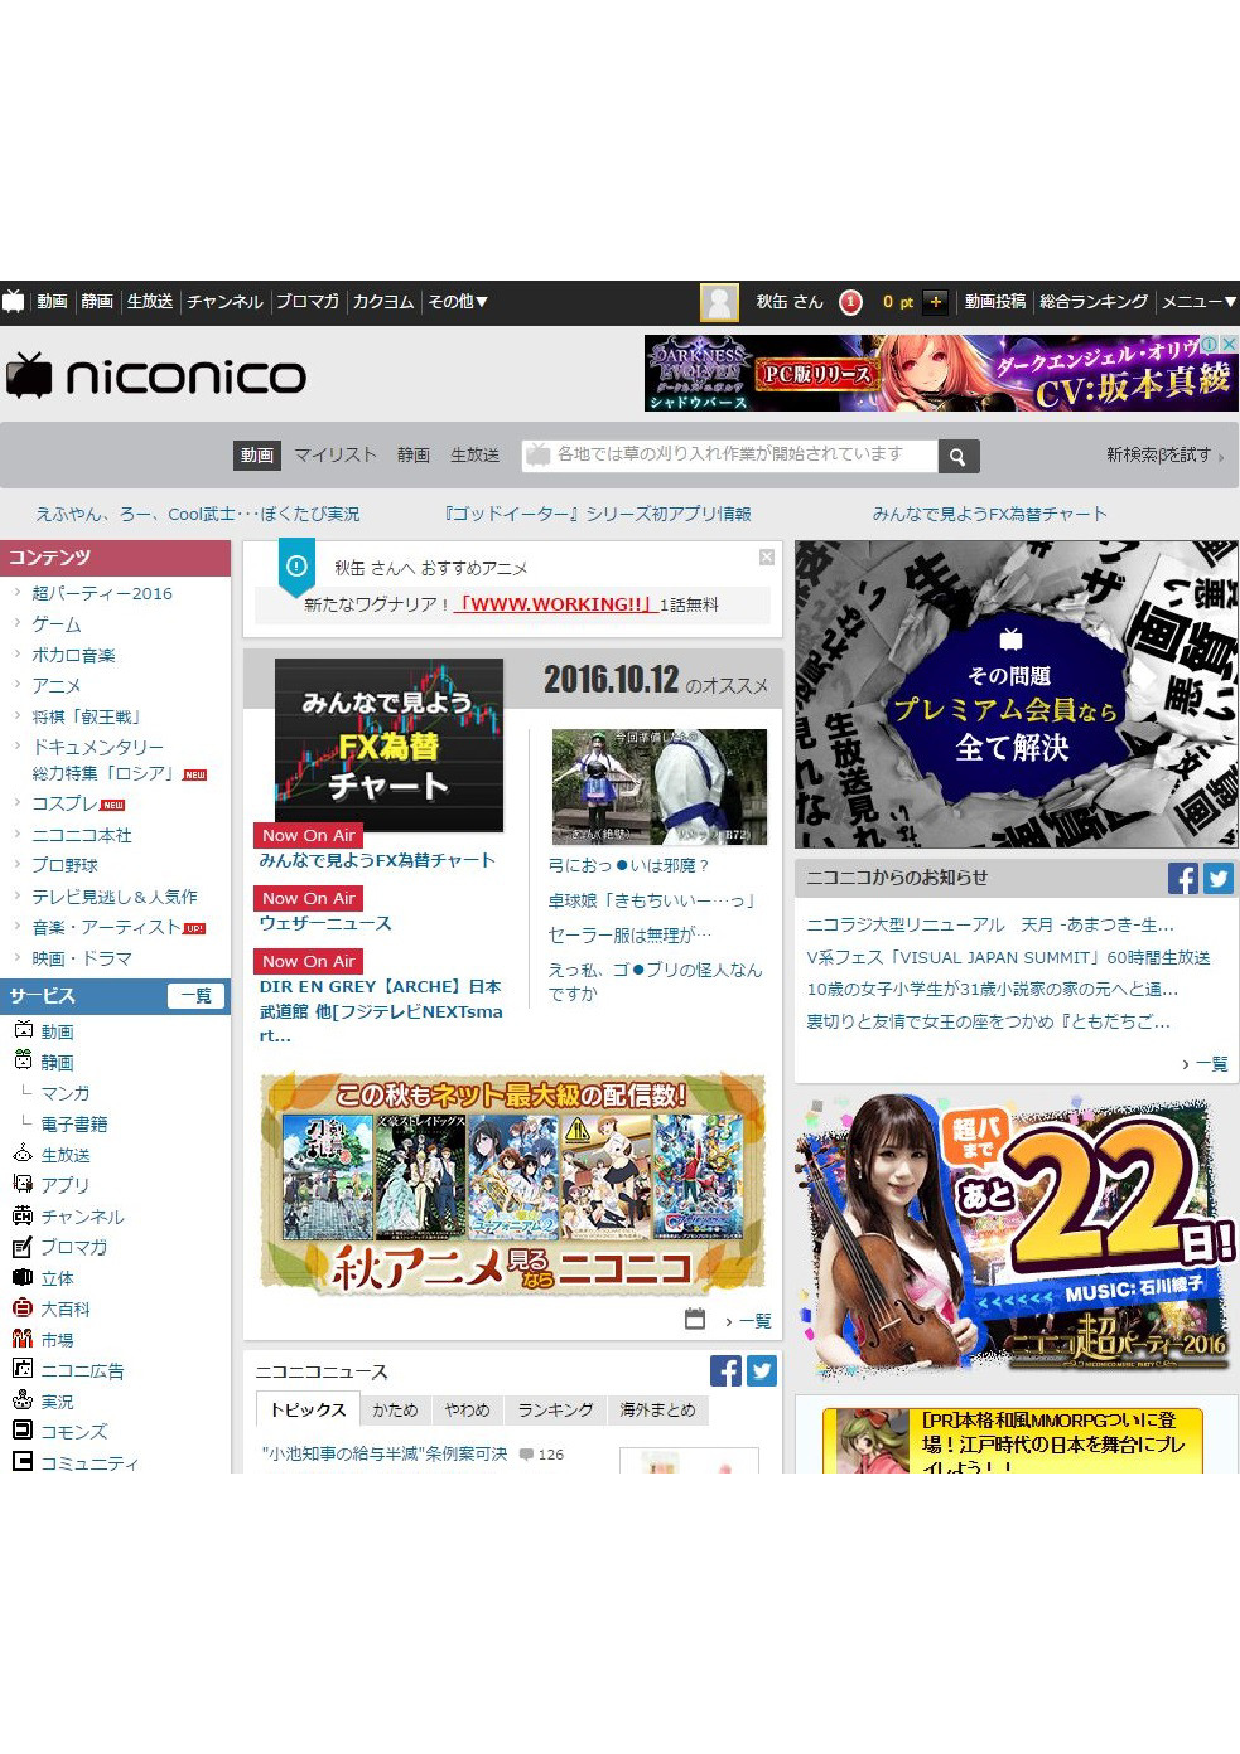
\includegraphics[width=14cm]{pppp.pdf}
\caption{ニコニコ動画のホームページ}\label{aaa}
\end{figure}


\clearpage

\section{用語}
ニコニコ動画で使用する用語に関して解説する.

\subsubsection*{ユーザー}
ニコニコ動画を利用している者を指す.

\subsubsection*{アカウント}
利用者はメールアドレスとパスワード,アカウント名を記入して登録する.

\subsubsection*{投稿者}
ニコニコ動画に動画を投稿した者を指す. 

\subsubsection*{視聴者}
ニコニコ動画に投稿された動画を視聴している者を指す.

\subsubsection*{投稿者コメント欄}
投稿者が自分の投稿した動画に対してコメント打つことが出来る欄を指す.コメントは投稿した動画にある投稿者メニューから編集できる.

\subsubsection*{再生数}
1つの動画に対して視聴者が再生を行った数.

\subsubsection*{マイリストページ}
アカウントのお気に入りやマイリスト,投稿,視聴履歴などを確認することができる.他にもアカウント設定の登録やプロフィールの表示確認・編集をすることもできる.

\begin{figure}[htb]
\centering
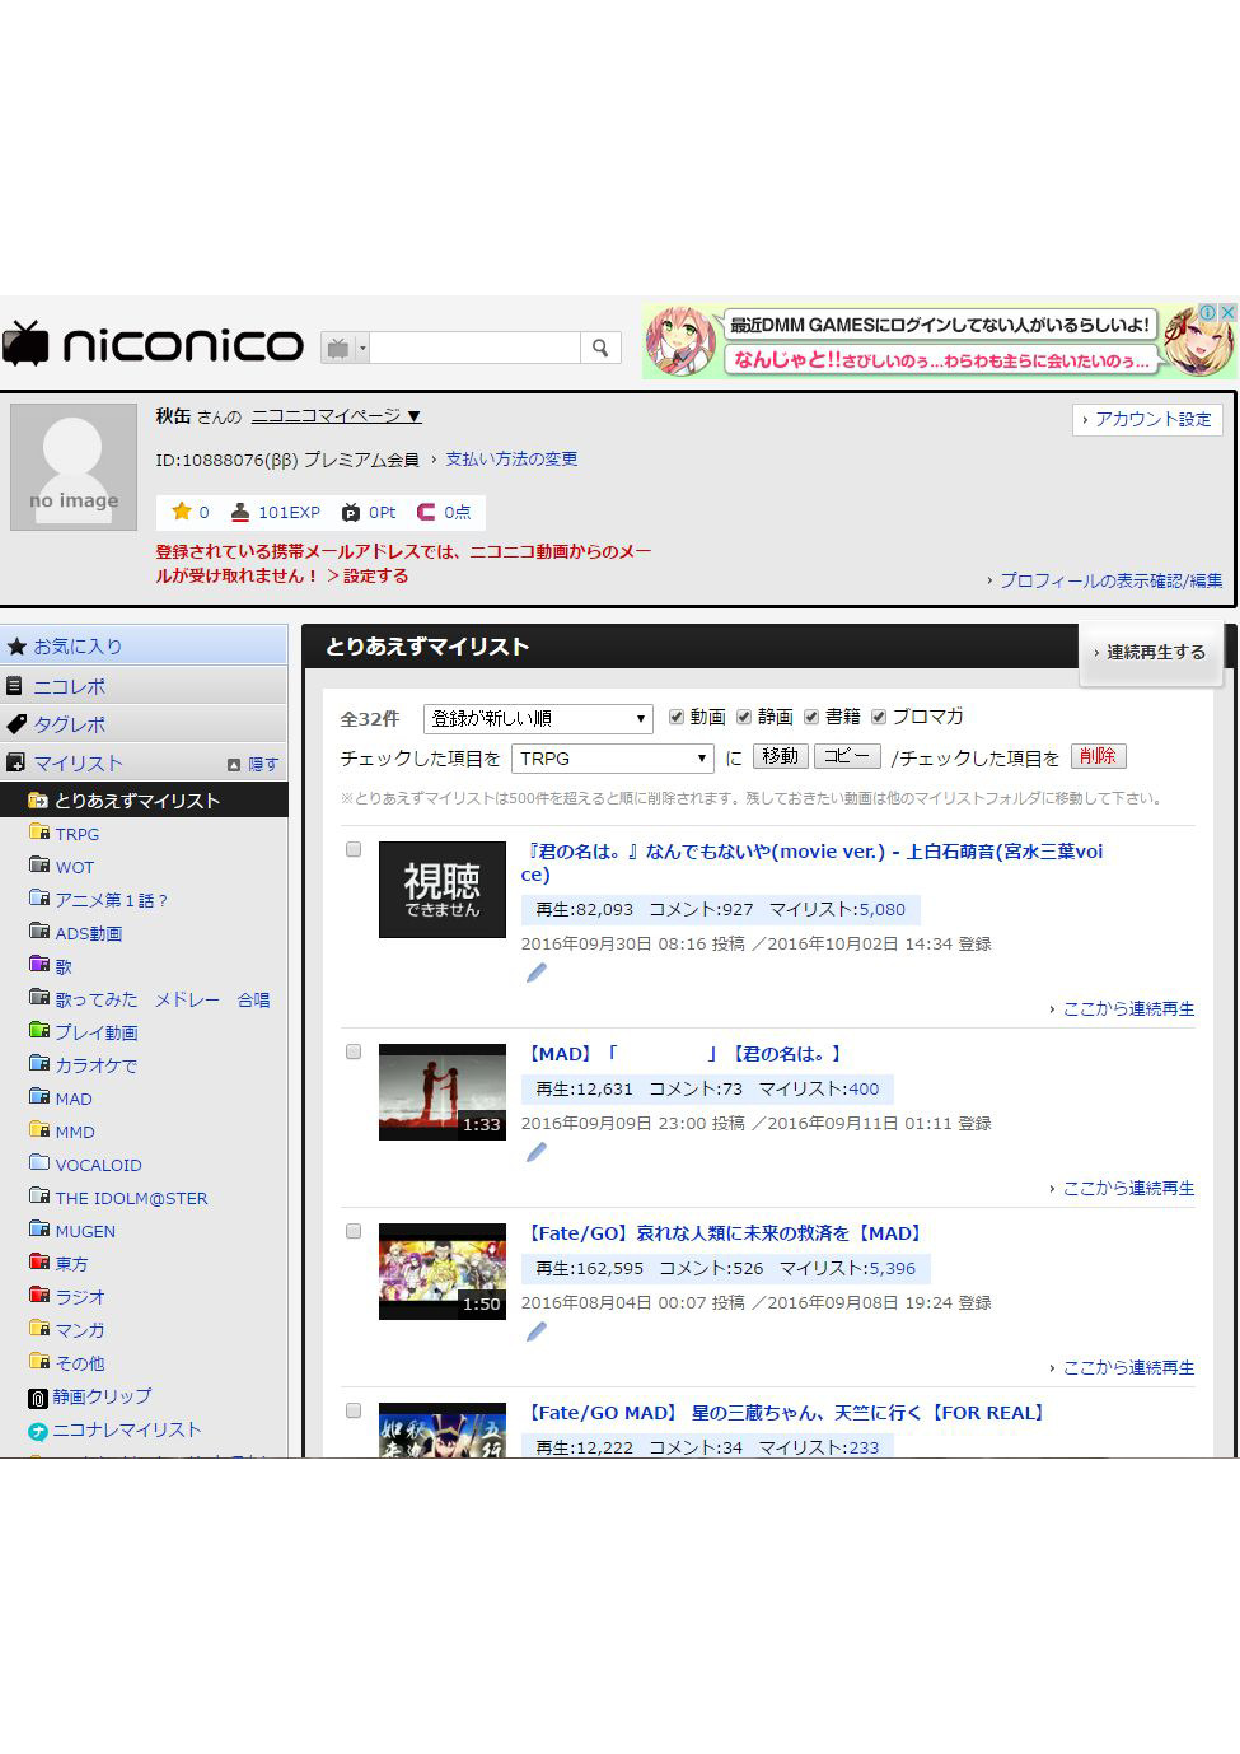
\includegraphics[width=14cm]{mairisuto.pdf}
\caption{マイリストページ}\label{mairisu}
\end{figure}


\clearpage
\subsubsection*{マイリスト}
視聴者がニコニコ動画内にある気に入った動画をブックマーク(お気に入り)として保存する機能.マイページでファイル名を変えられるファイルがありこのファイル1つを選択して入れることが出来る.ほかのファイルに同じ動画をマイリストすることもできる.

\subsubsection*{とりあえずマイリスト}
名前を決めたファイルに入れずにとっておくことがきるマイリストのこと.このリストにお気に入り動画がある場合,動画のマイリスト数にカウントされない.

\subsubsection*{マイリスト数}
1つの動画に対して視聴者がブックマークした数.ただし,とりあえずマイリストに動画がある場合,カウントされることはない.

\subsubsection*{コメント}
投稿された動画に対してユーザーが打ち込む.打ち込まれたコメントは動画内で表示される.

\subsubsection*{コメント数}
1つの動画に対して視聴者が打ち込んだコメントの数.

\subsubsection*{タグ}
動画に付箋のような分類分けをすることができる機能.ユーザーが変えることができる.

\subsubsection*{広告}
ニコニコポイントを消費して,ユーザーが動画または生放送を宣伝することができる.他にも使用期限が存在するが公式からチケットが配られ,これをニコニコポイントの代わりに使うこともできる.

\subsubsection*{視聴履歴}
使っているアカウントで見た動画を最大100件まで記録されており,90日前の履歴を記録している.

\subsubsection*{お気に入り}
投稿されている動画の投稿者アカウント名下にあるお気に入り登録ボタンをクリックすることによって,お気に入り登録することができる.

\subsubsection*{ニコニコ総合ランキング}
ニコニコで見られている映画ランキングやAmebaで見られている動画ランキング,ユーザーが宣伝している動画ランキングなどの様々なランキングがある.

\subsubsection*{ニコニコ動画ランキング}
エンタメ・音楽や生活・一般・スポーツ,政治などのカテゴリーでランキングしたもの.期間別として毎時,24時間,週刊,月間,合計がある.対象として総合,再生,コメント,マイリストがある.

\subsubsection*{ニコニコレポート}
ユーザー自身がお気に入りしたユーザーやチャンネル,コミュニティで動画を投稿したり,生放送を行ったりすると,自身のニコニコレポートに表示される.

\begin{figure}[htb]
\centering
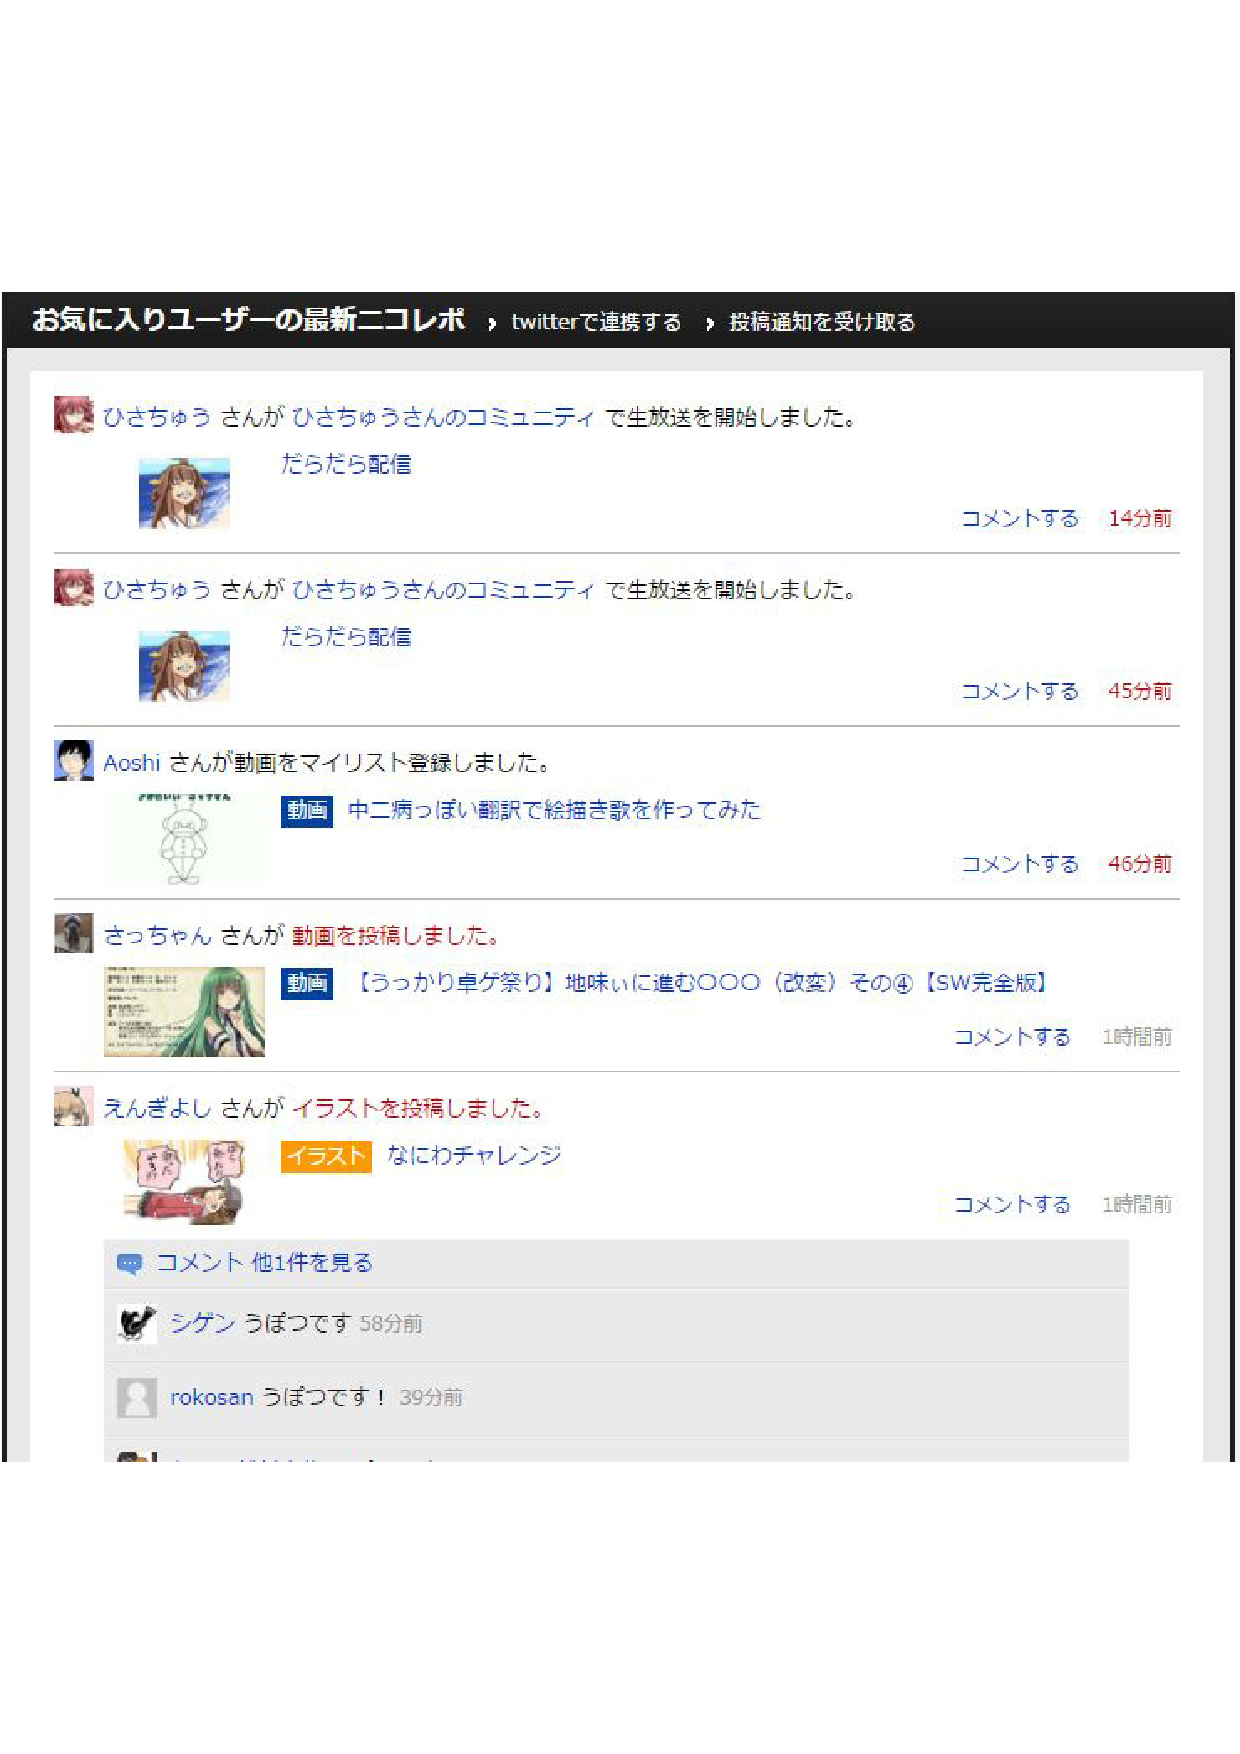
\includegraphics[width=14cm]{nikorepo.pdf}
\caption{ニコニコレポート}\label{nikorepo}
\end{figure}

\section{カテゴリ合算毎時総合ランキングとは}
ニコニコ動画ランキングのカテゴリーを合算し,毎時間更新し,再生数やコメント数,マイリスト数などを総合してランキングにしたもの.今回の研究ではこのランキングからデータを回収する.

\begin{figure}[htb]
\centering
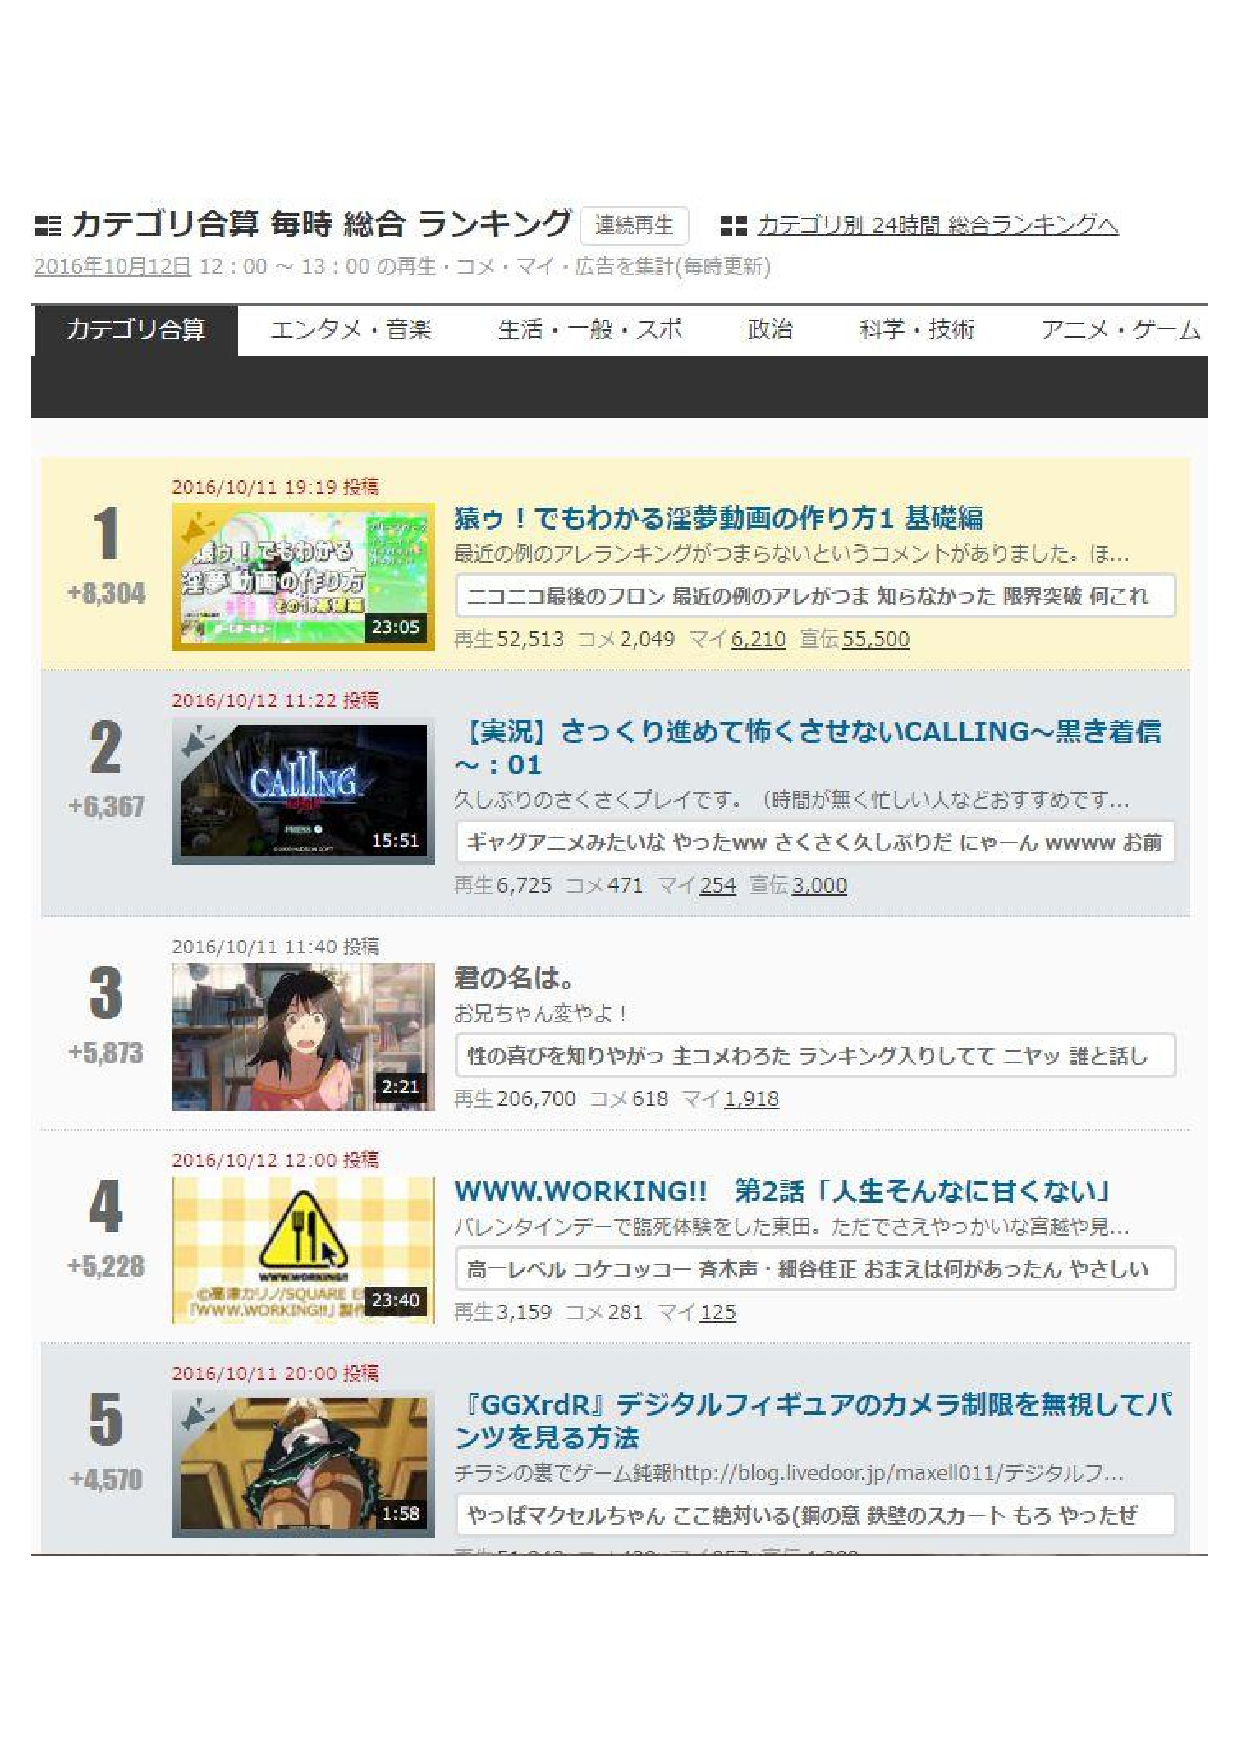
\includegraphics[width=7cm]{r01.pdf}
\caption{カテゴリ合算毎時総合ランキング}\label{aab}
\end{figure}

\begin{figure}[htb]
\centering
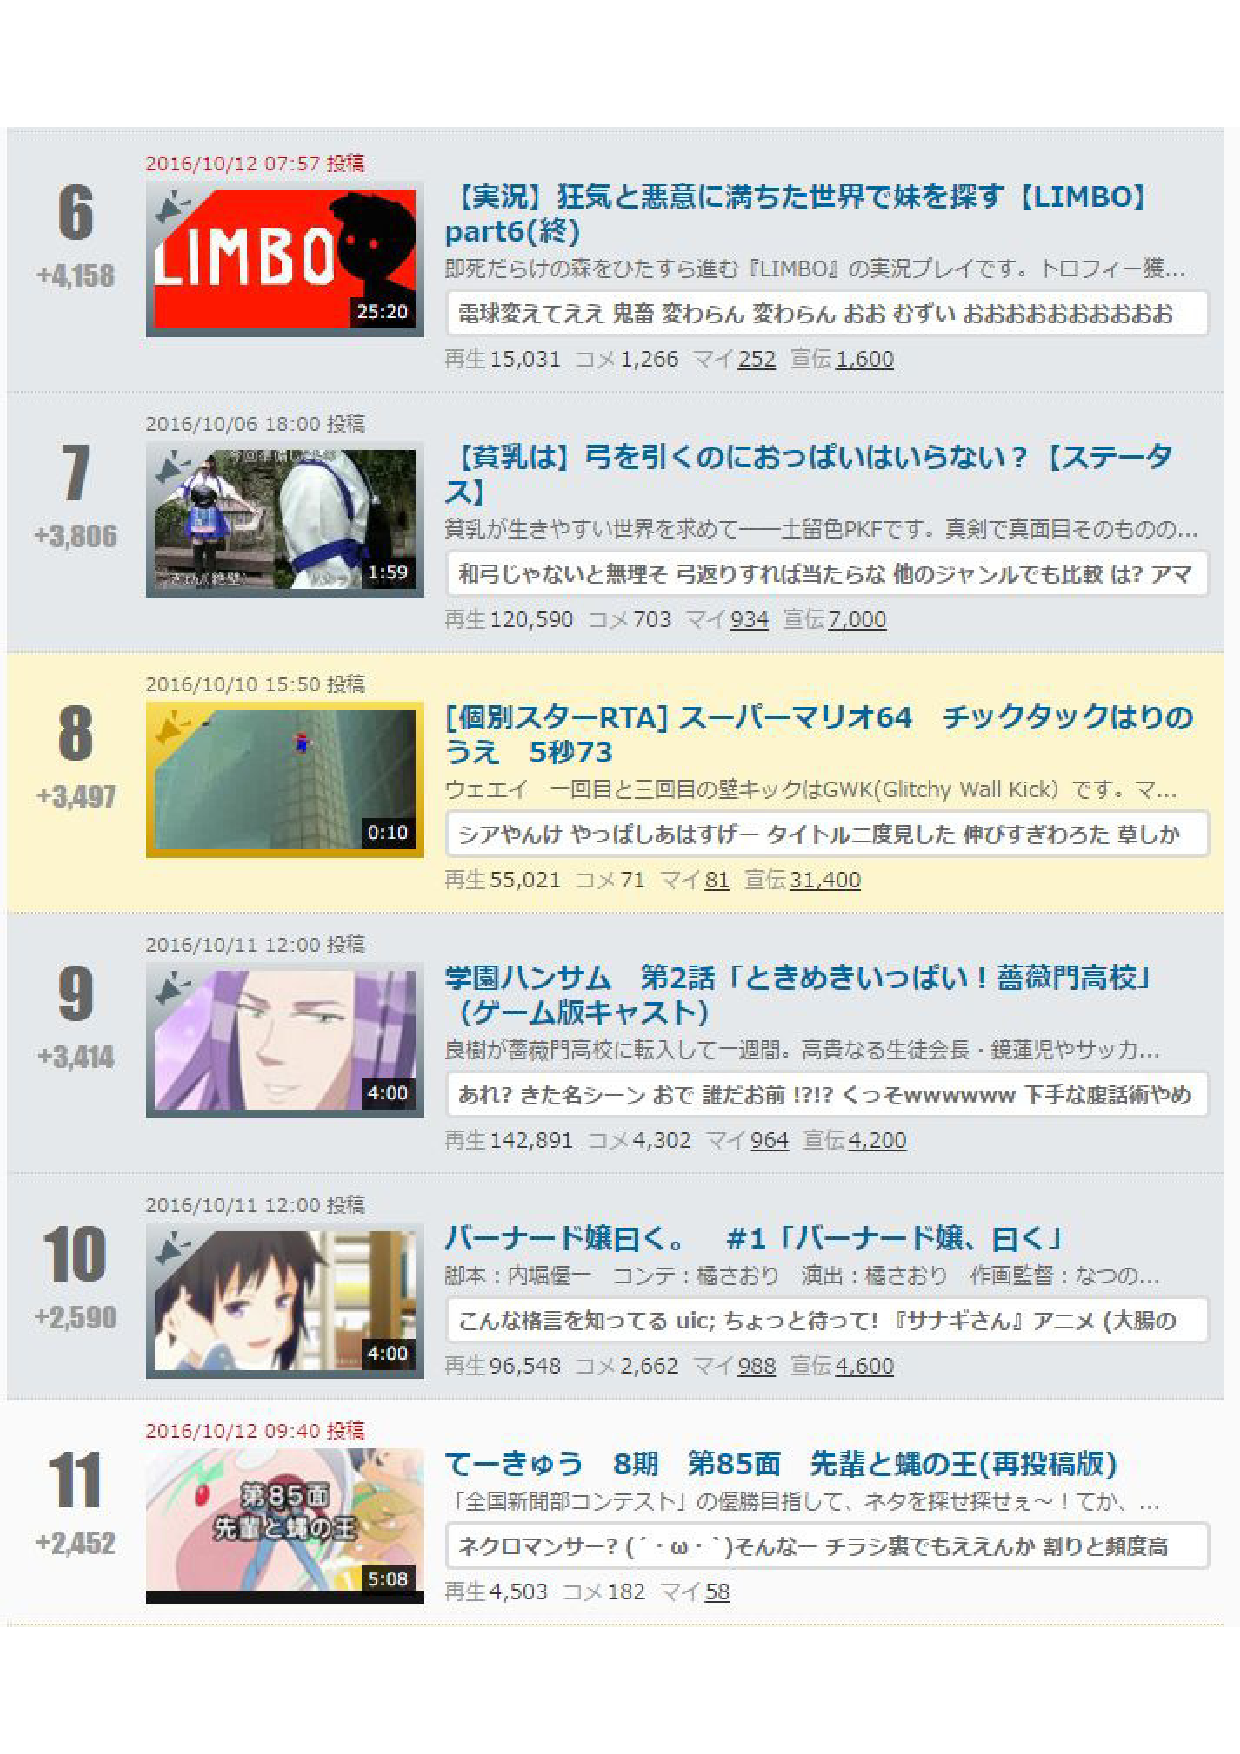
\includegraphics[width=7cm]{r02.pdf}
\caption{カテゴリ合算毎時総合ランキング}\label{aac}
\end{figure}

\begin{figure}[htb]
\centering
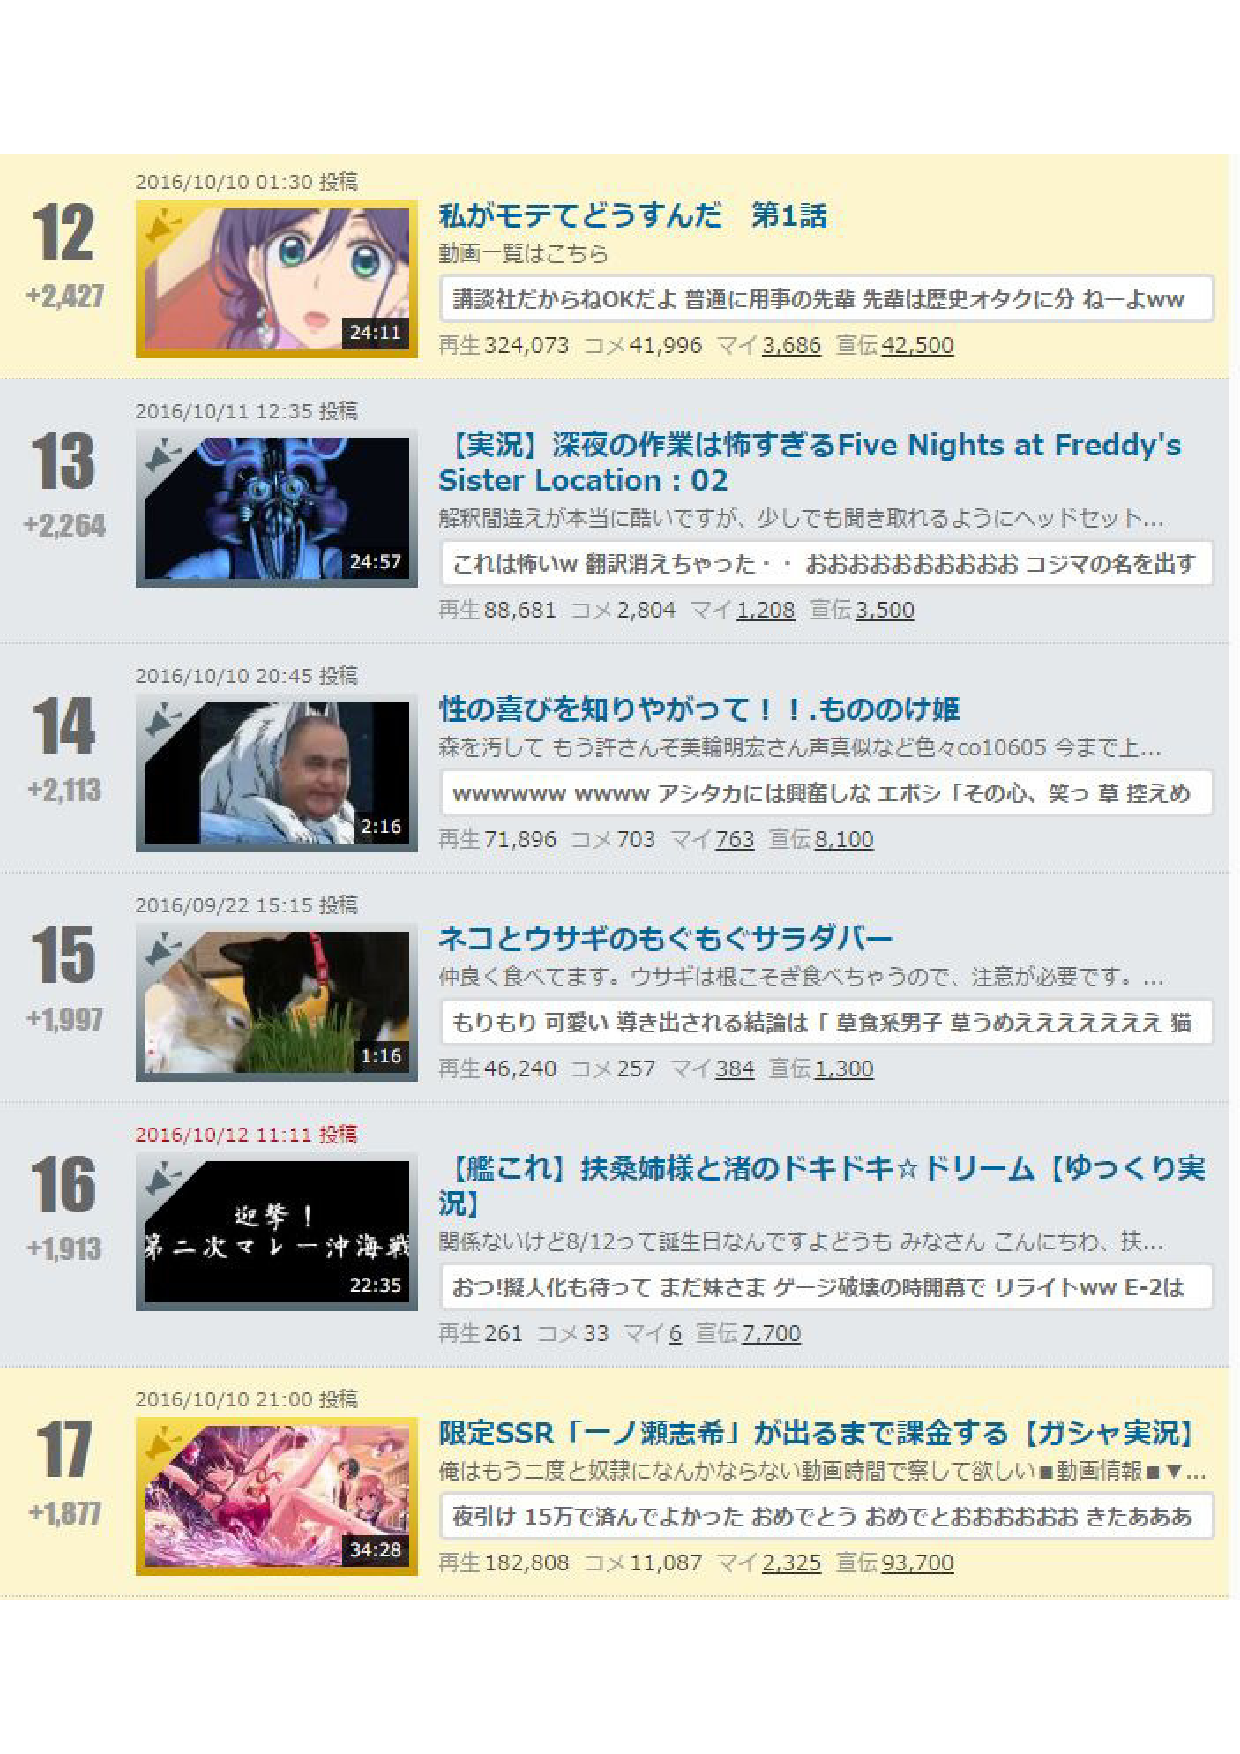
\includegraphics[width=7cm]{r03.pdf}
\caption{カテゴリ合算毎時総合ランキング}\label{aad}
\end{figure}

\begin{figure}[htb]
\centering
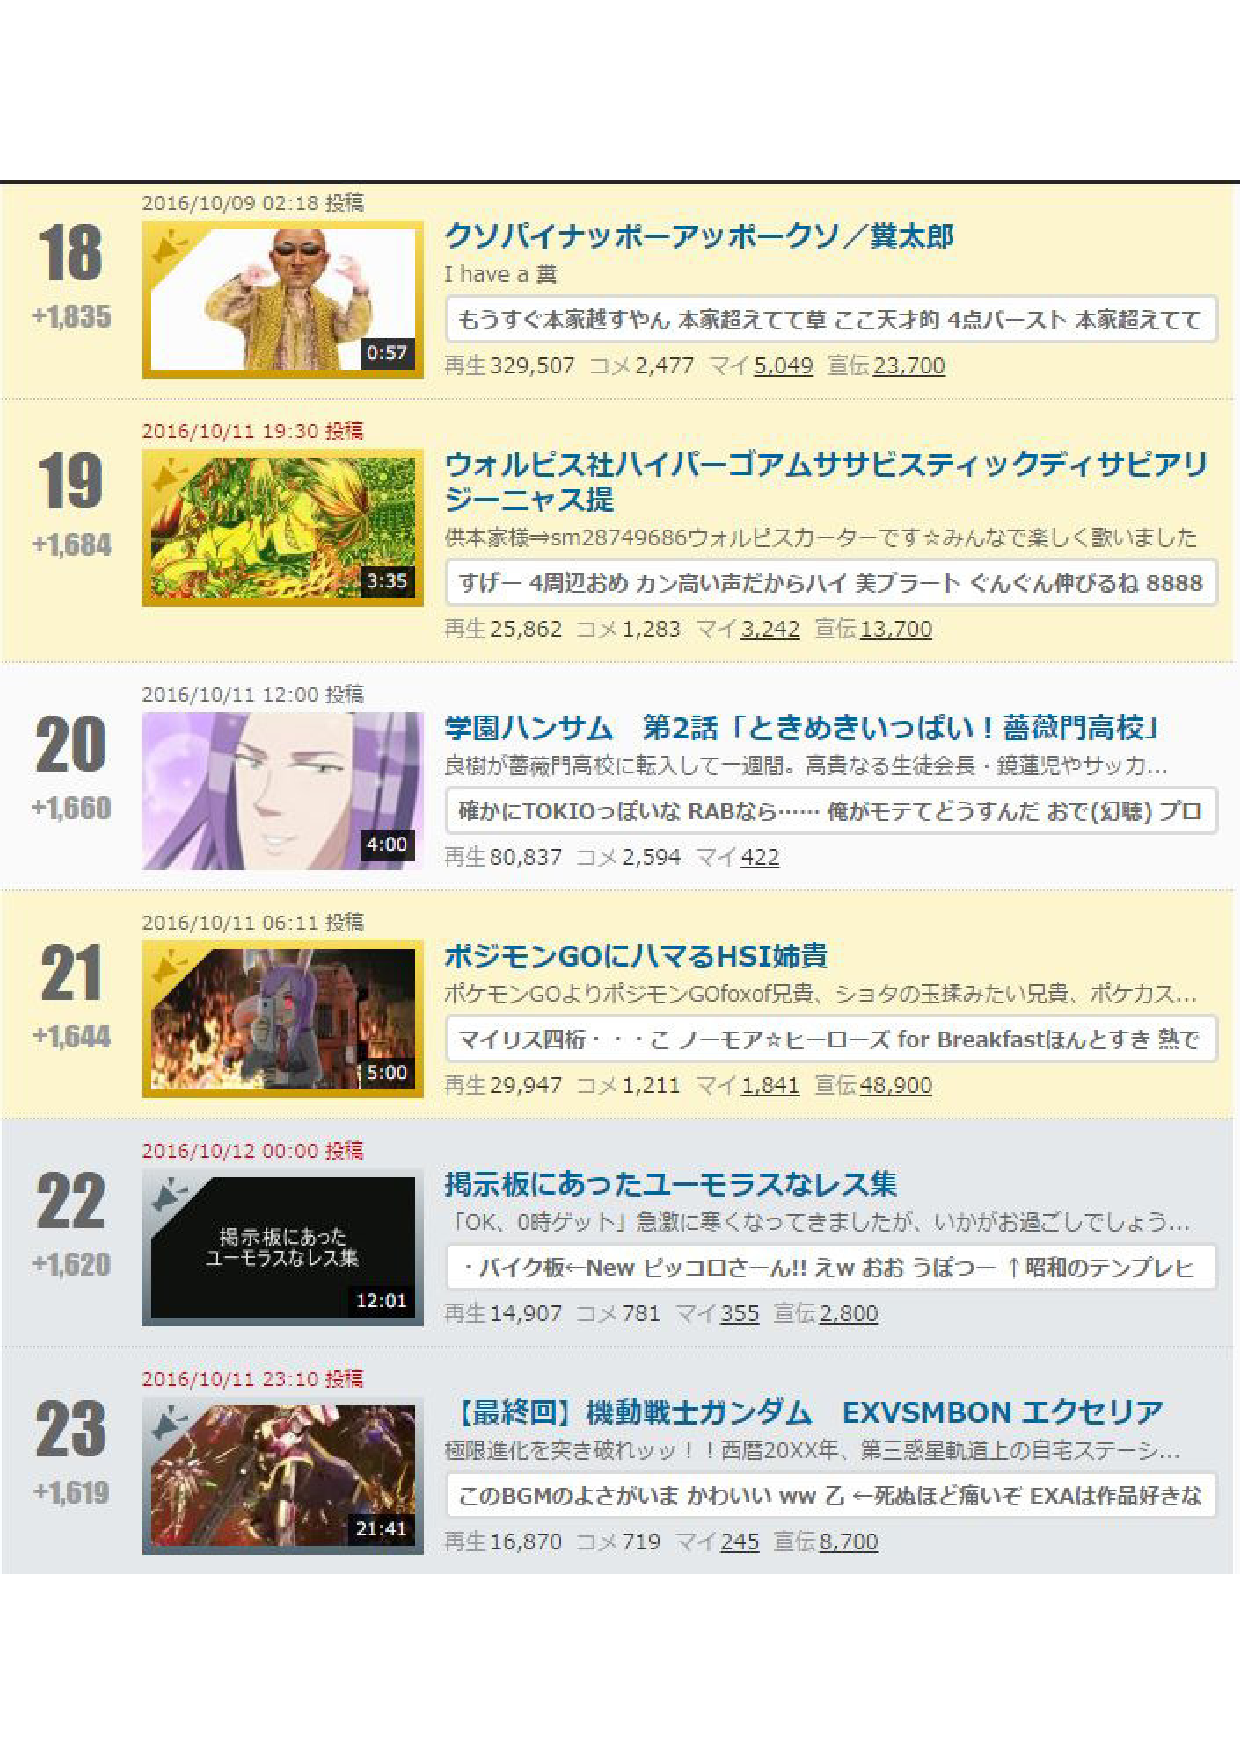
\includegraphics[width=7cm]{r04.pdf}
\caption{カテゴリ合算毎時総合ランキング}\label{aae}
\end{figure}

\begin{figure}[htb]
\centering
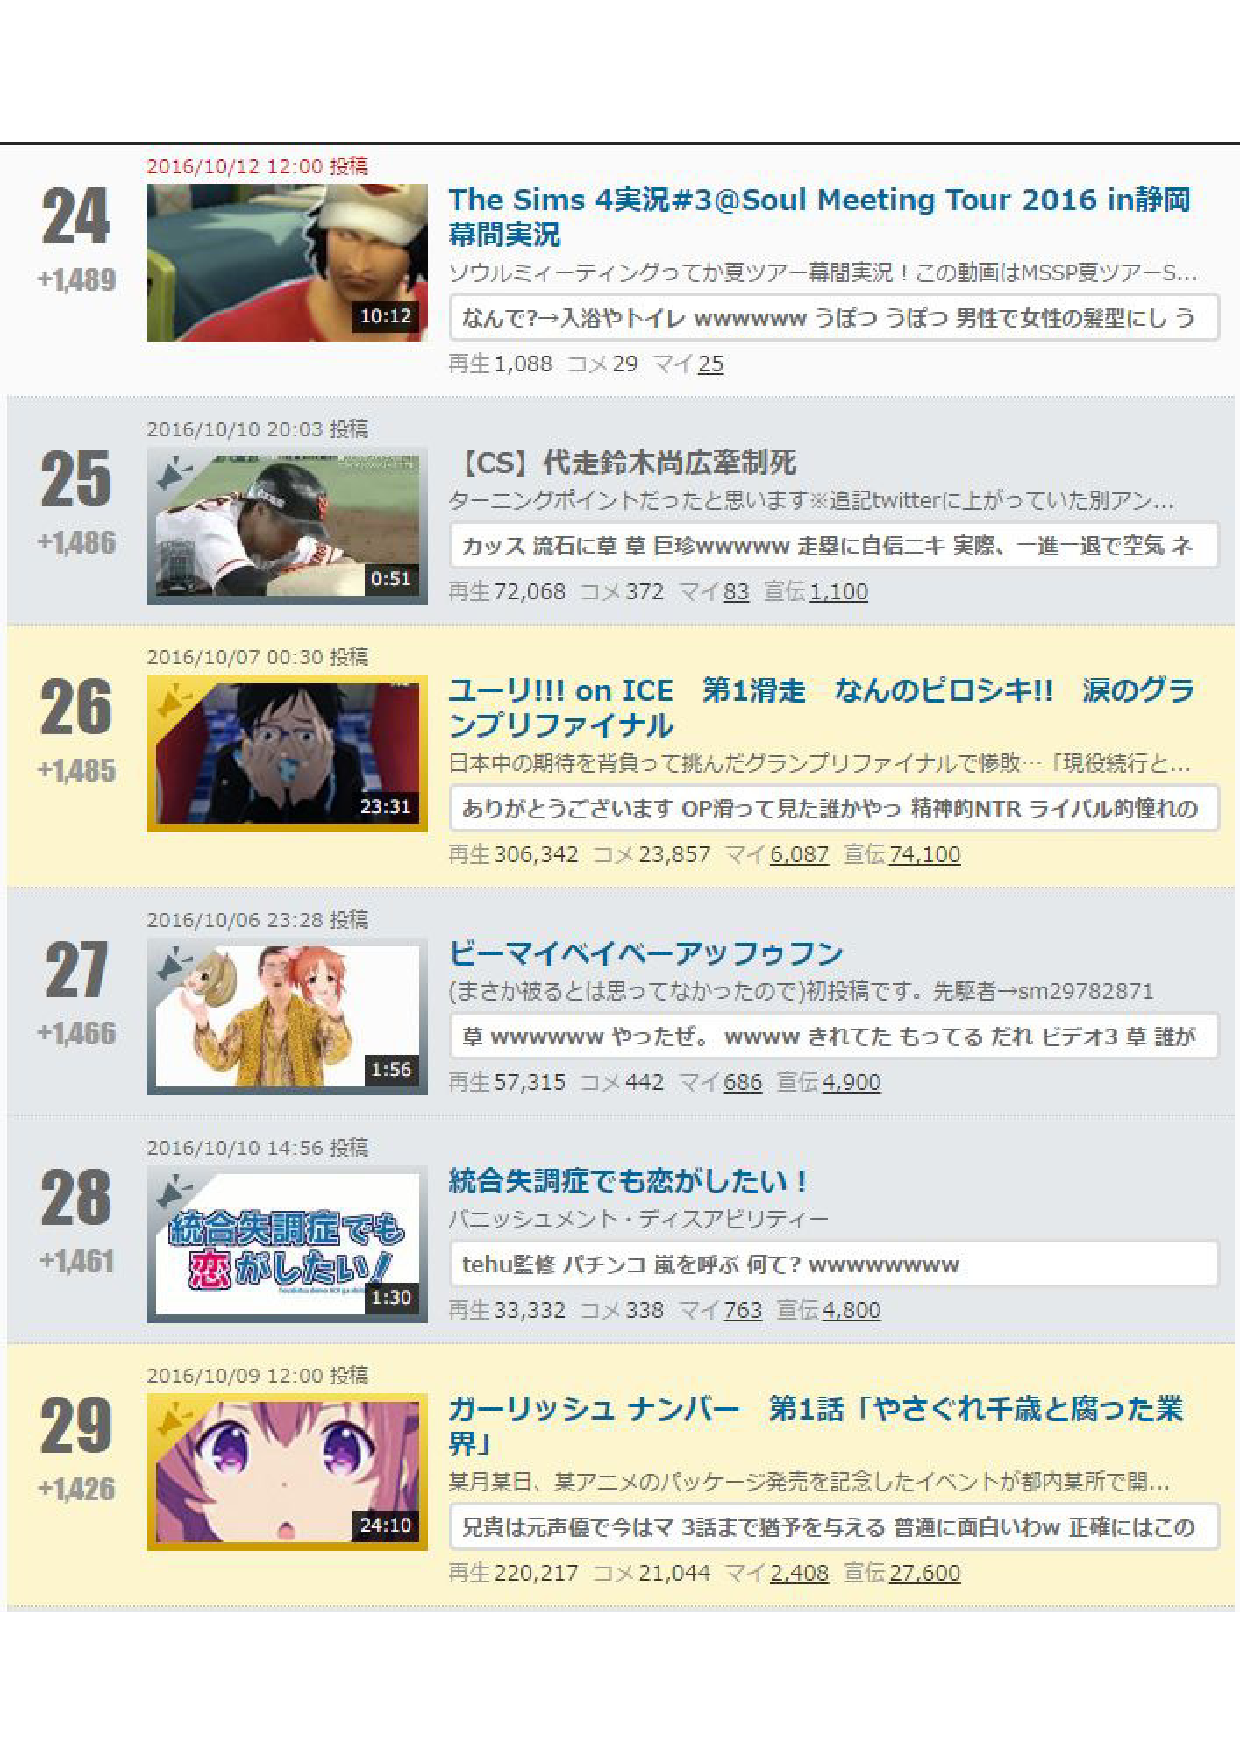
\includegraphics[width=7cm]{r05.pdf}
\caption{カテゴリ合算毎時総合ランキング}\label{aaf}
\end{figure}

\begin{figure}[htb]
\centering
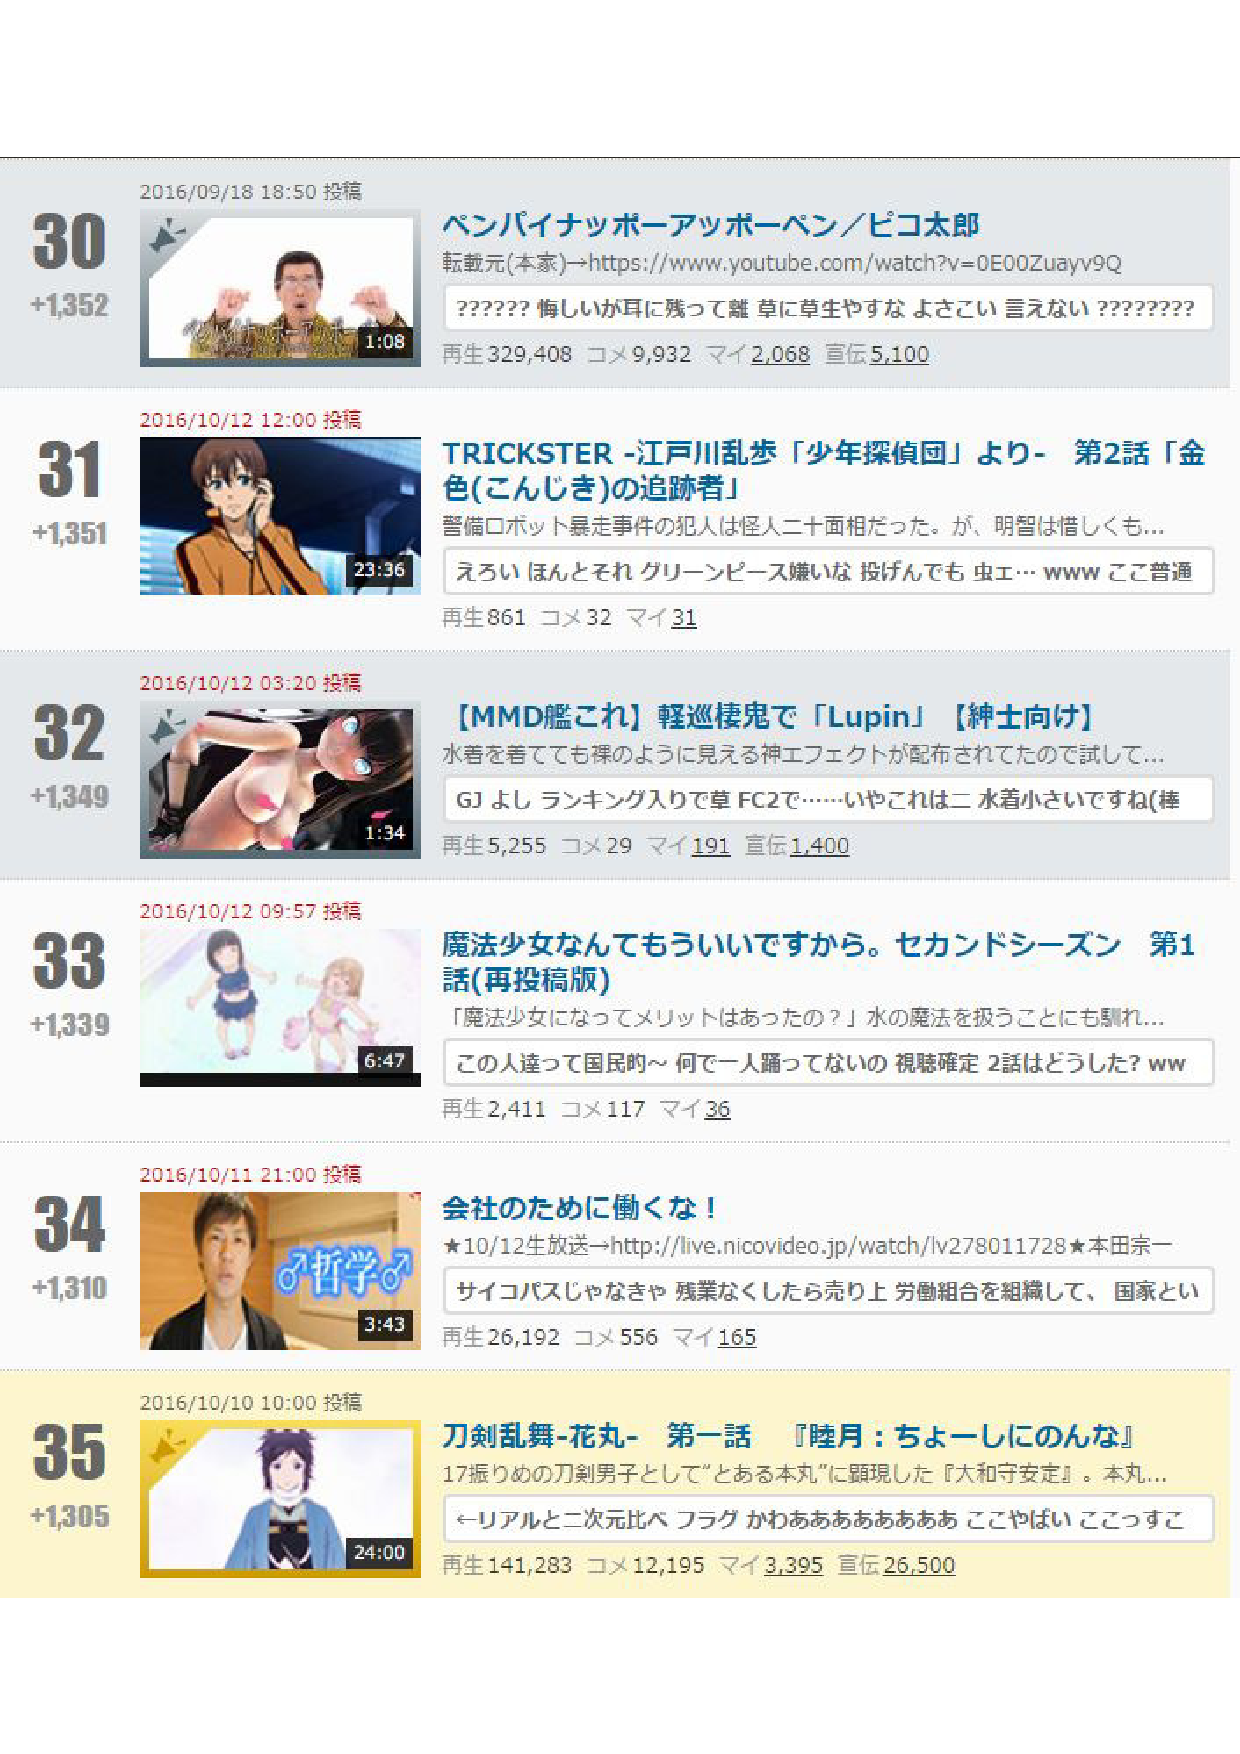
\includegraphics[width=7cm]{r06.pdf}
\caption{カテゴリ合算毎時総合ランキング}\label{aag}
\end{figure}

\begin{figure}[htb]
\centering
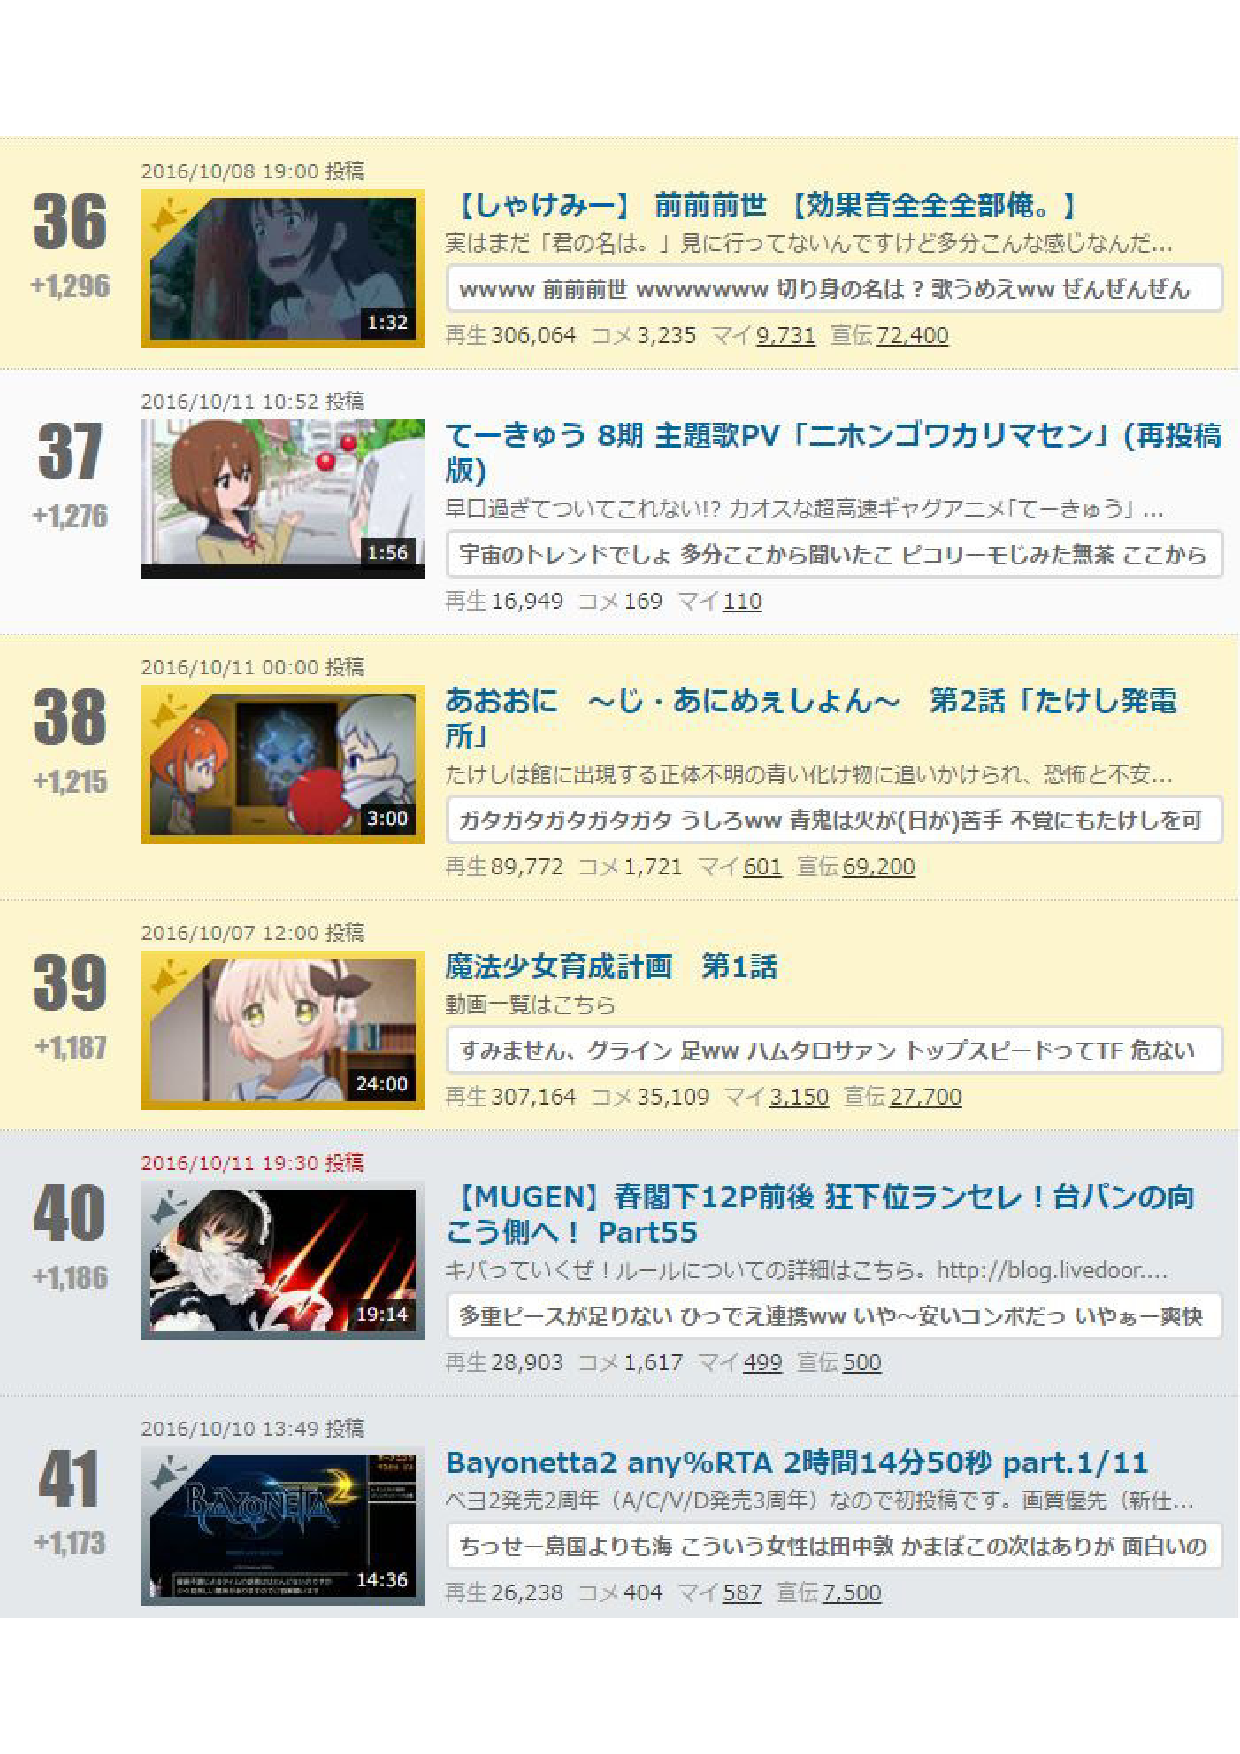
\includegraphics[width=7cm]{r07.pdf}
\caption{カテゴリ合算毎時総合ランキング}\label{aba}
\end{figure}

\begin{figure}[htb]
\centering
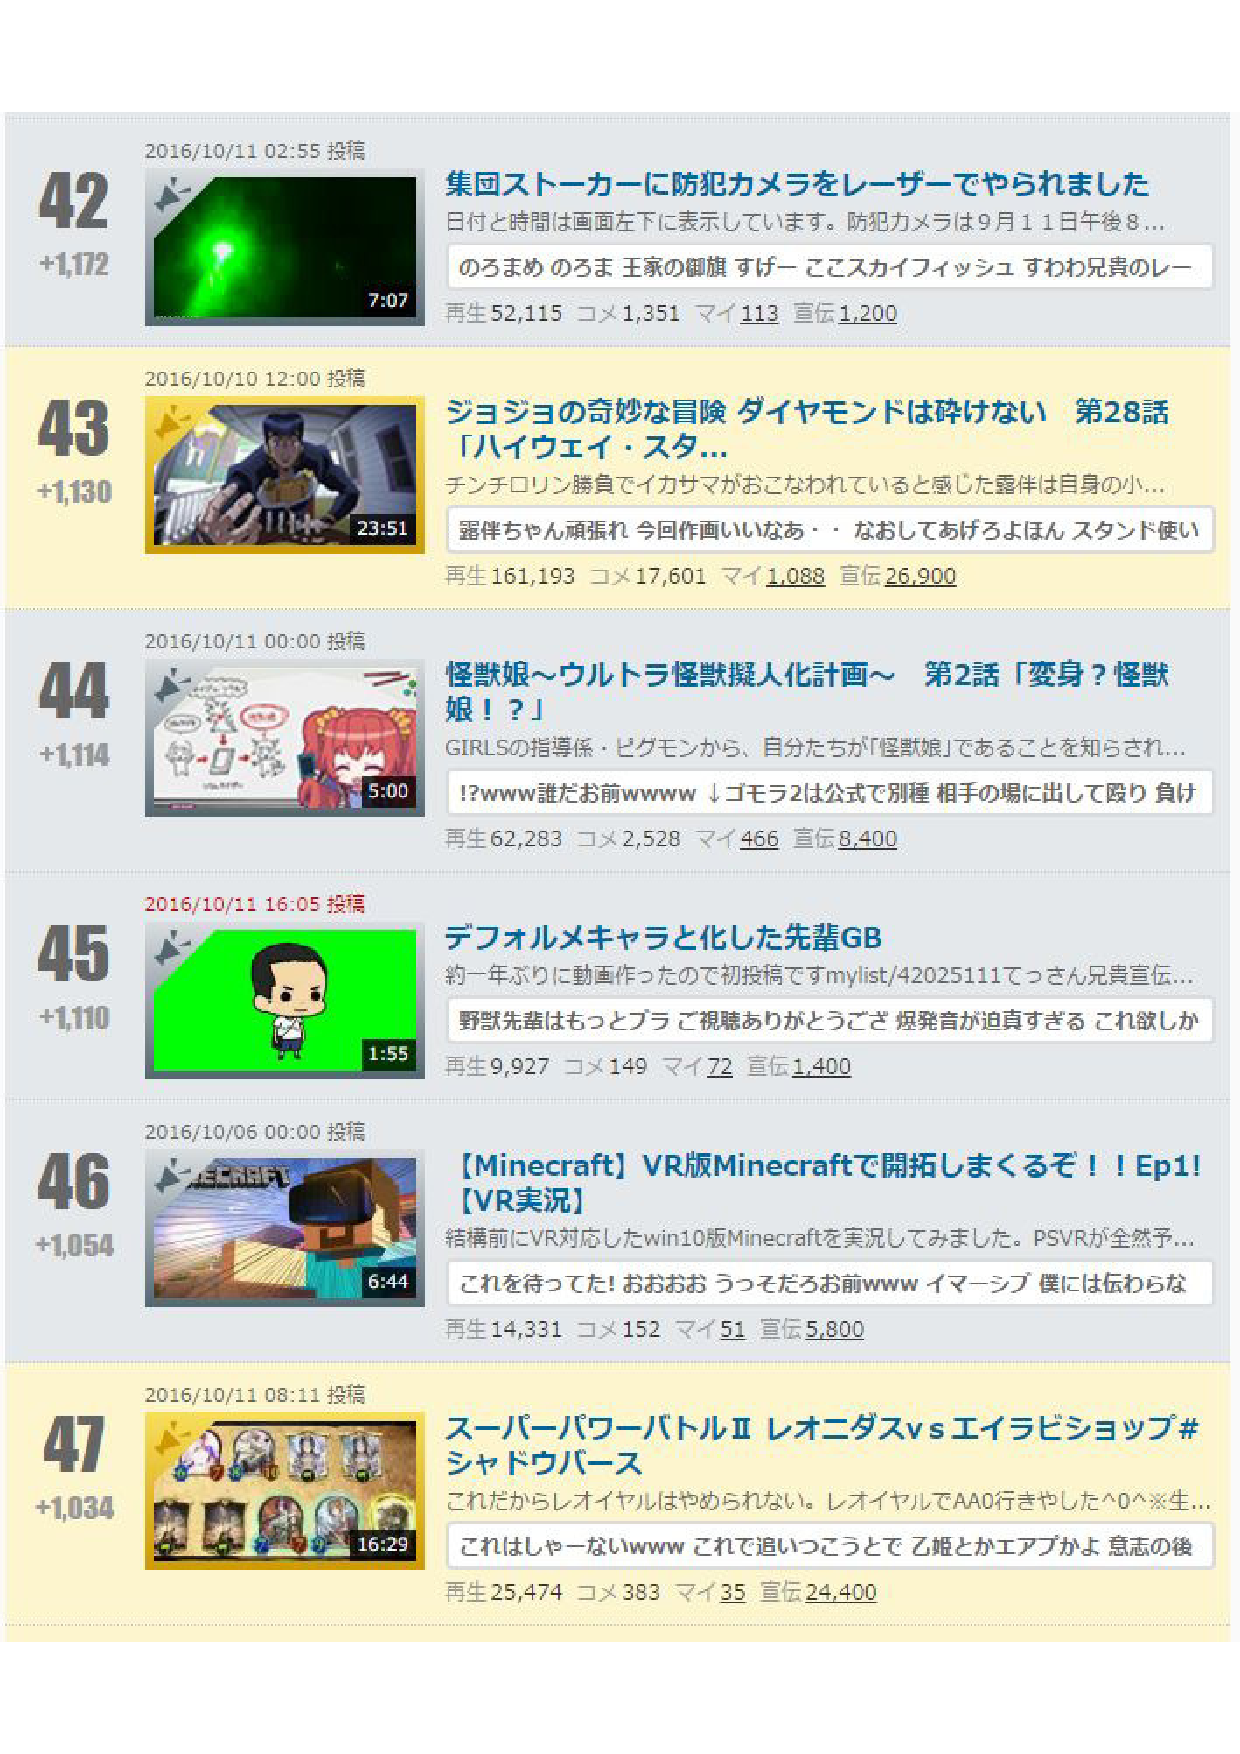
\includegraphics[width=7cm]{r08.pdf}
\caption{カテゴリ合算毎時総合ランキング}\label{abb}
\end{figure}

\begin{figure}[htb]
\centering
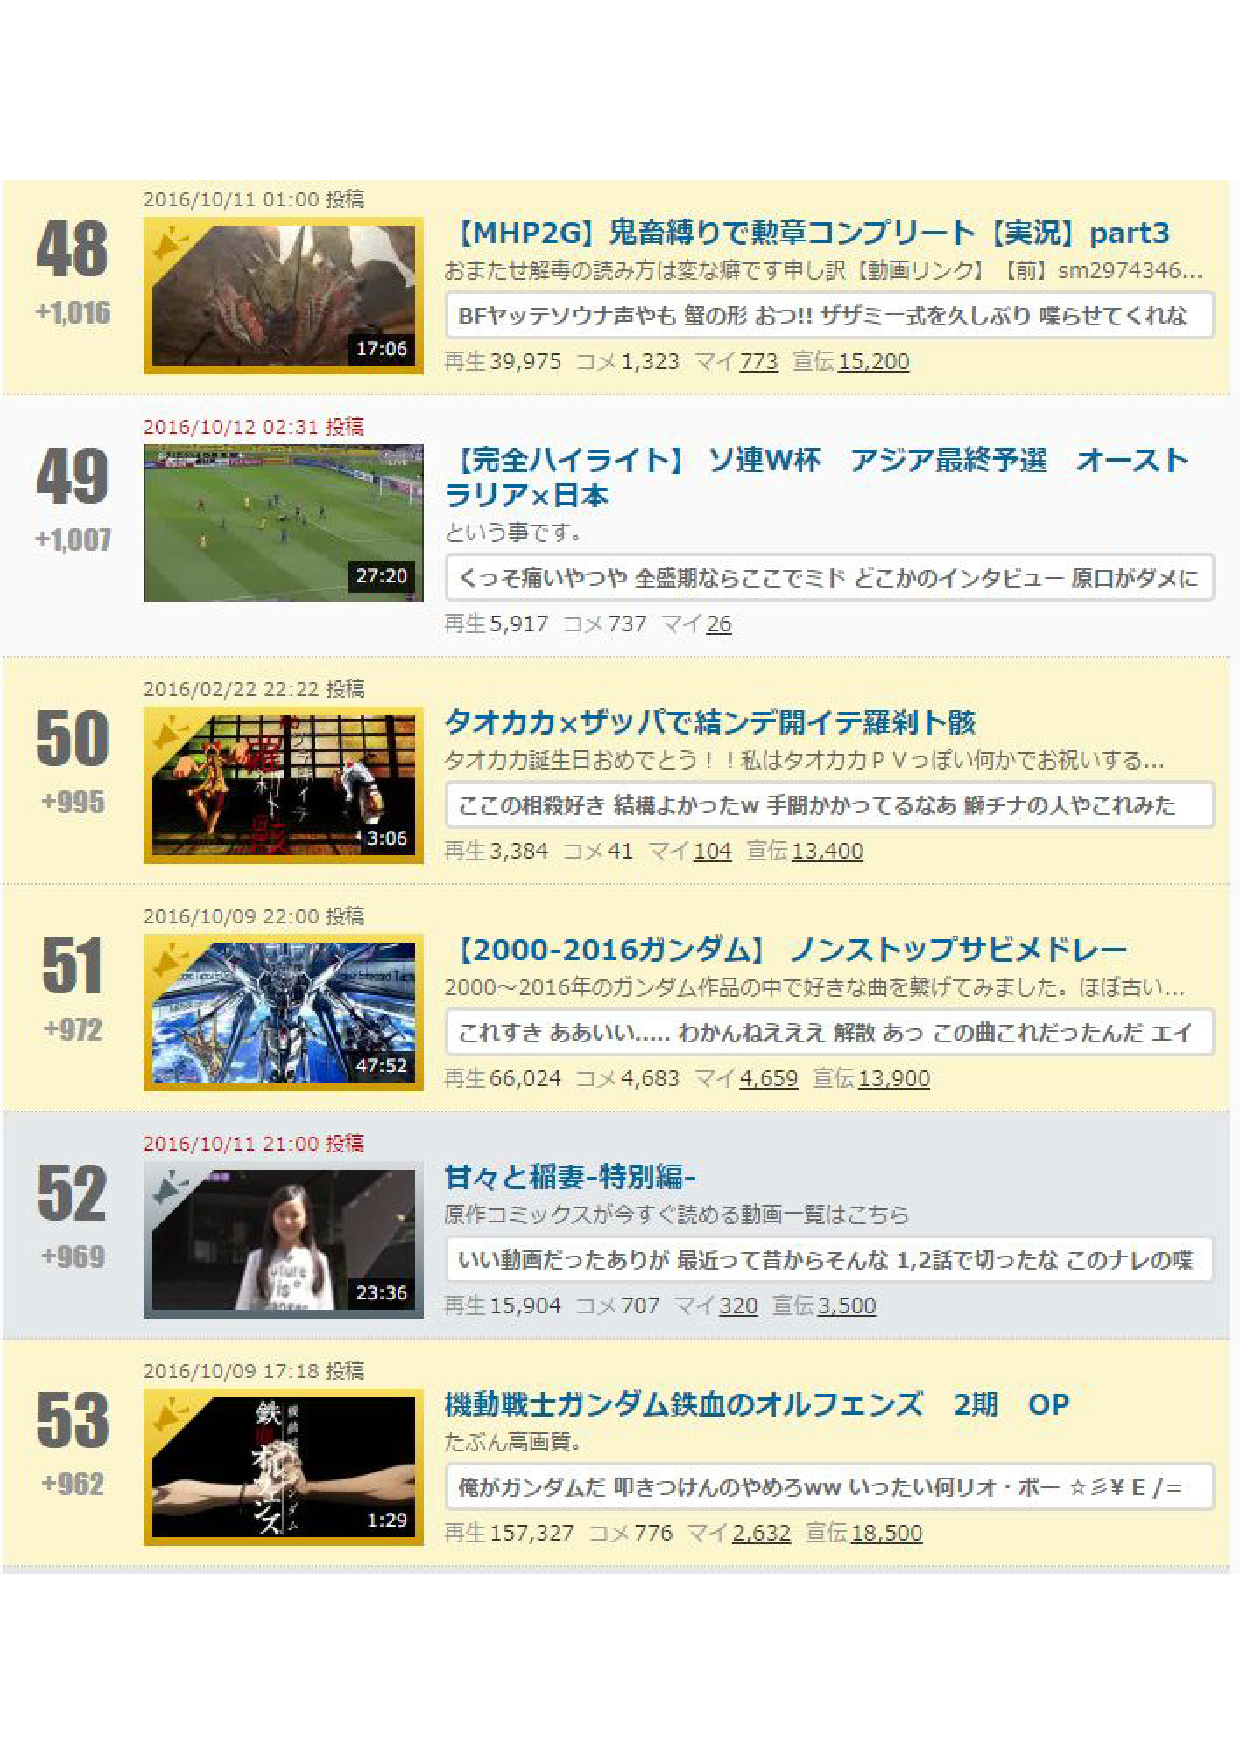
\includegraphics[width=7cm]{r09.pdf}
\caption{カテゴリ合算毎時総合ランキング}\label{abc}
\end{figure}

\begin{figure}[htb]
\centering
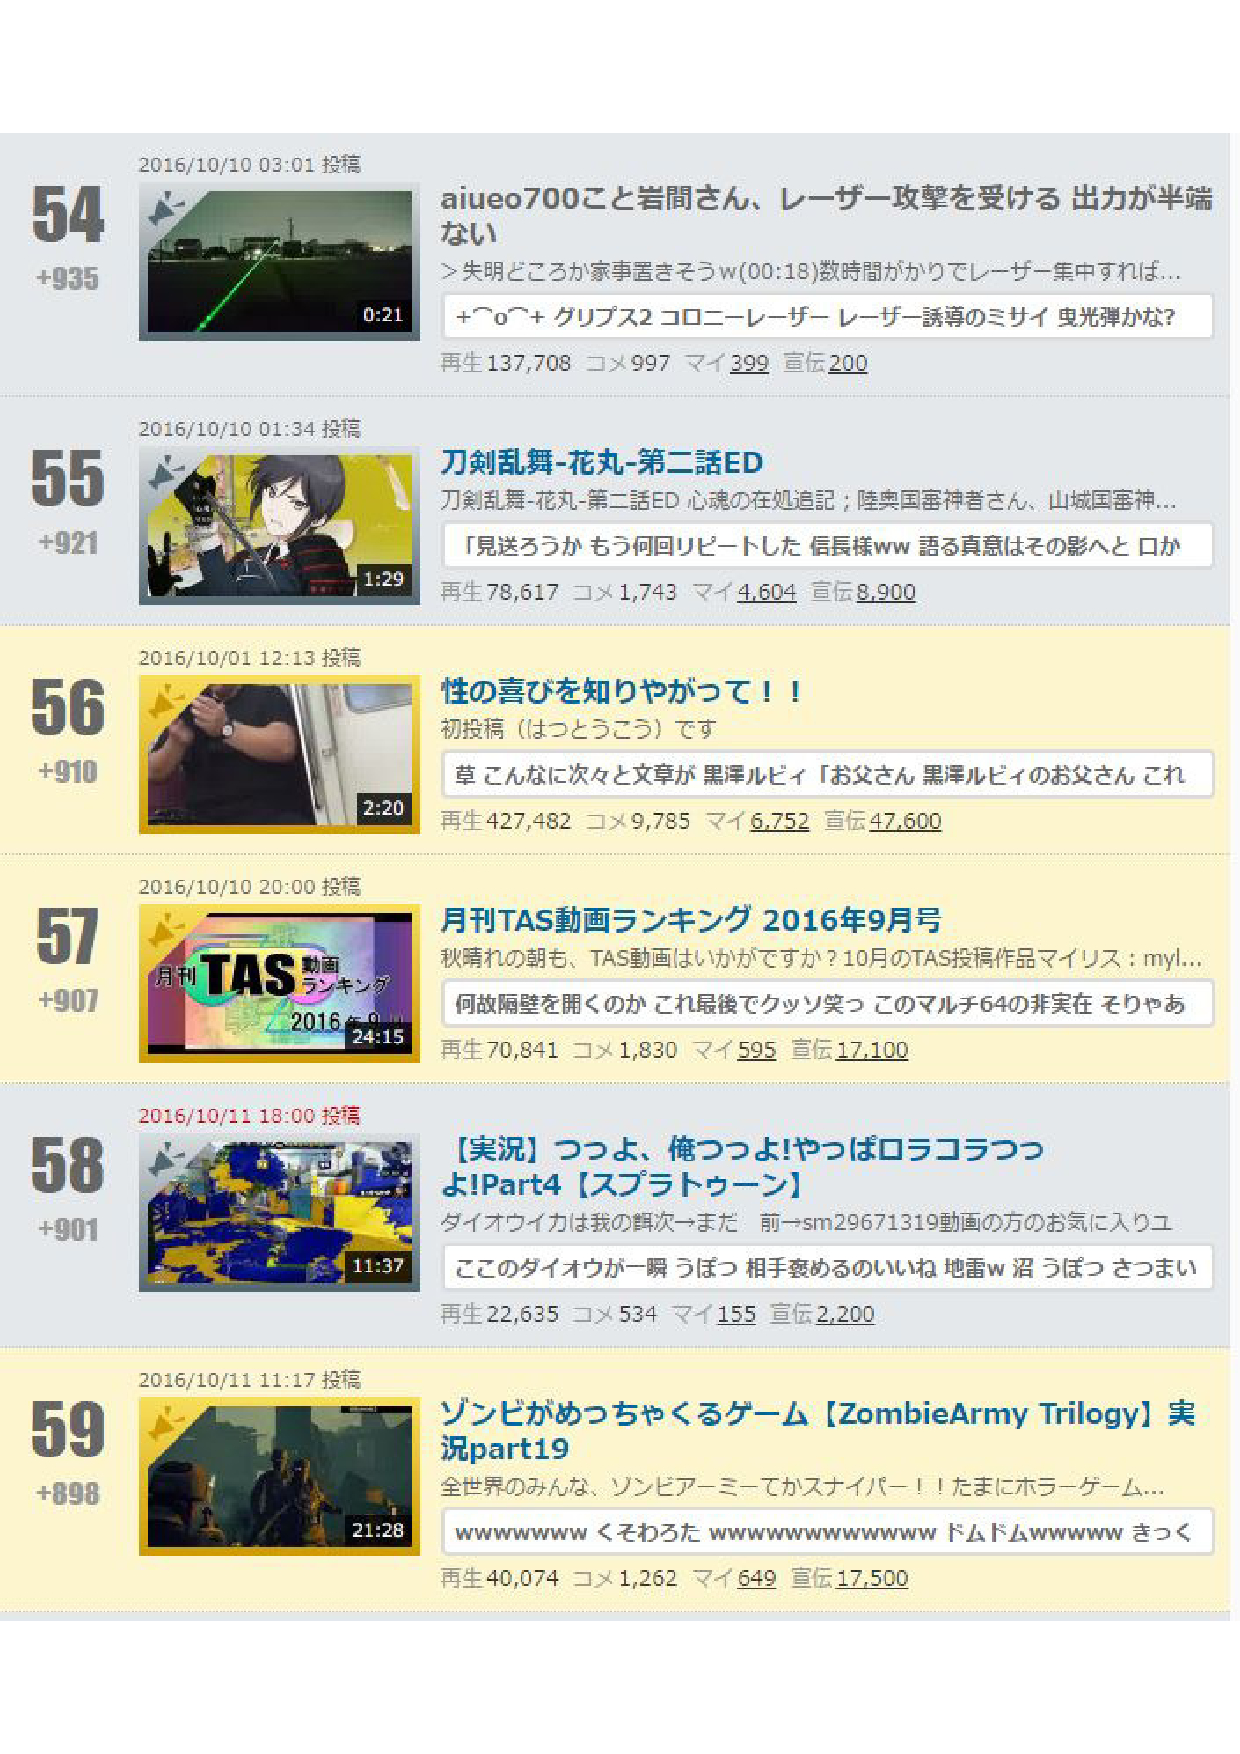
\includegraphics[width=7cm]{r10.pdf}
\caption{カテゴリ合算毎時総合ランキング}\label{abd}
\end{figure}

\begin{figure}[htb]
\centering
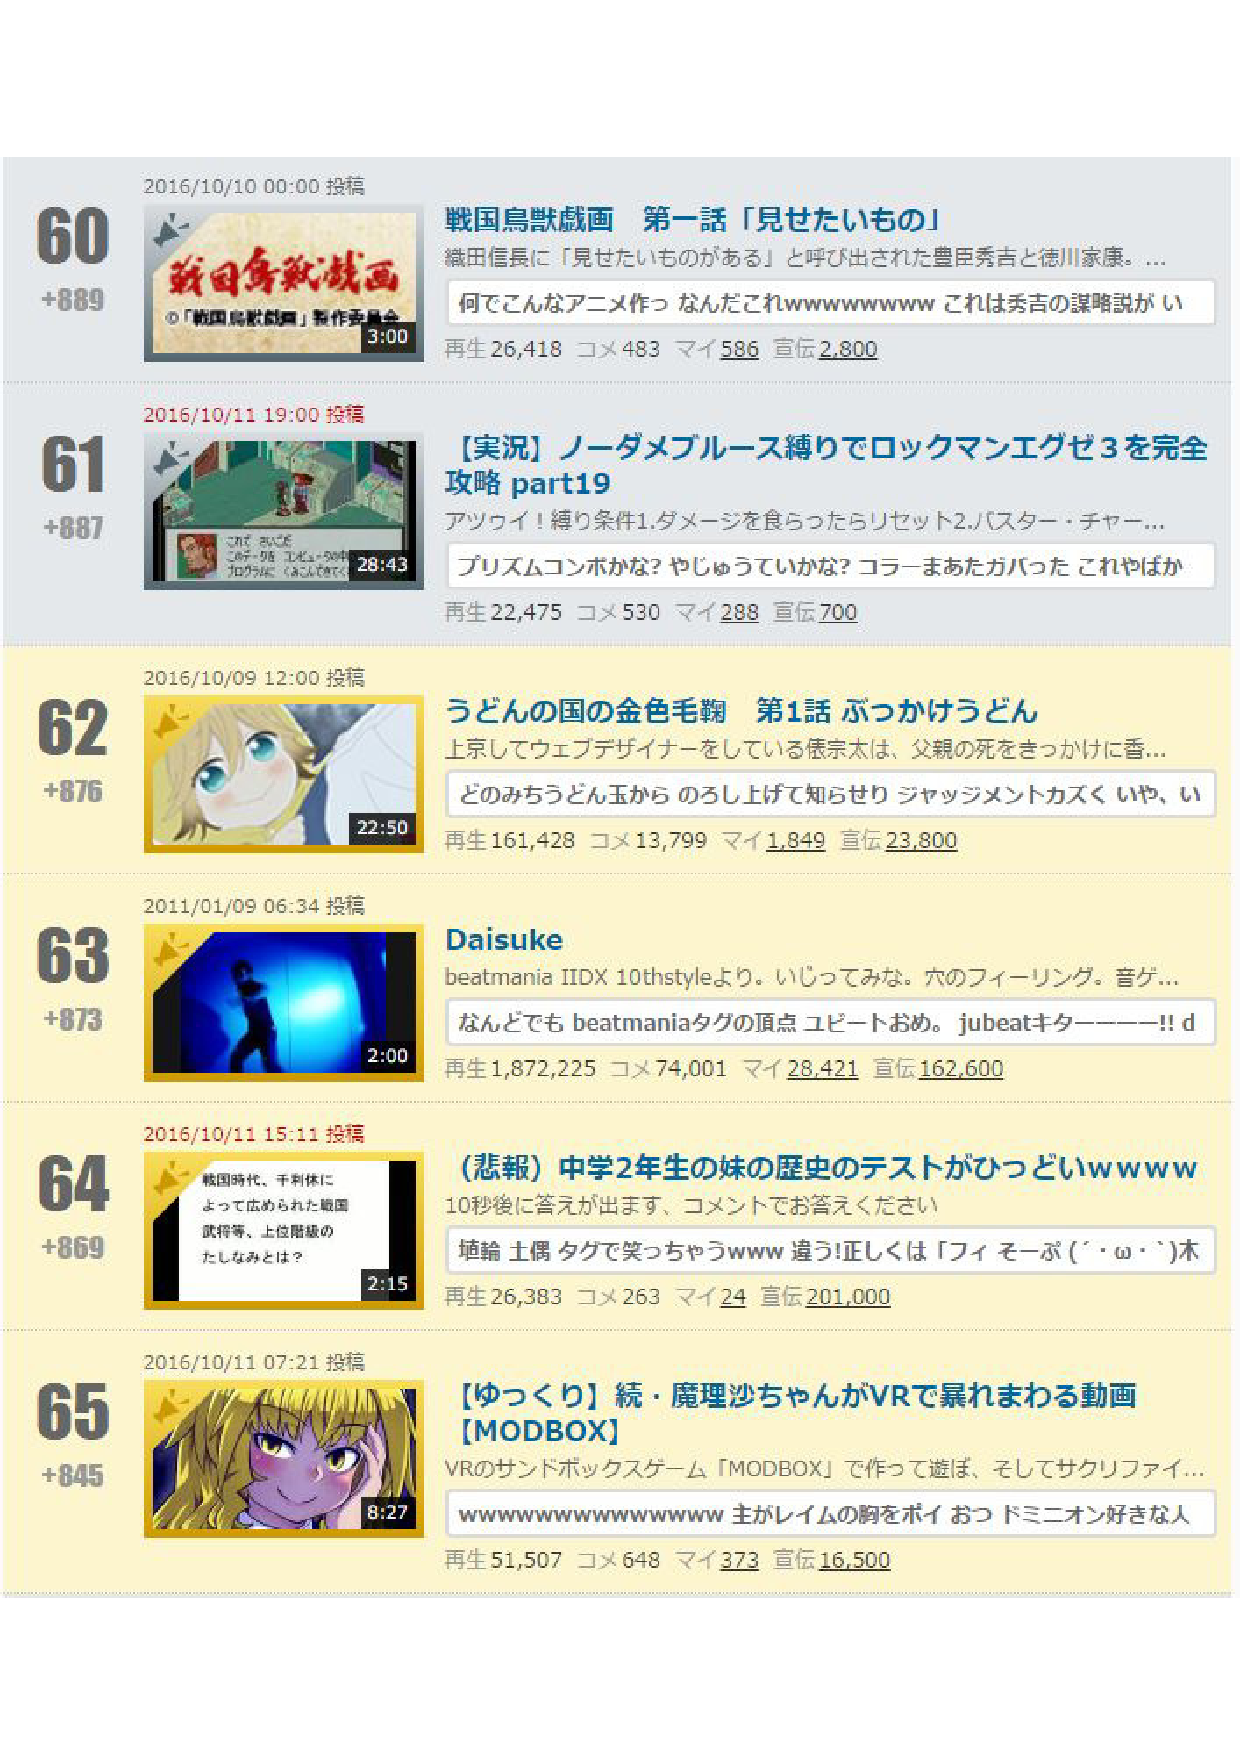
\includegraphics[width=7cm]{r11.pdf}
\caption{カテゴリ合算毎時総合ランキング}\label{abe}
\end{figure}

\begin{figure}[htb]
\centering
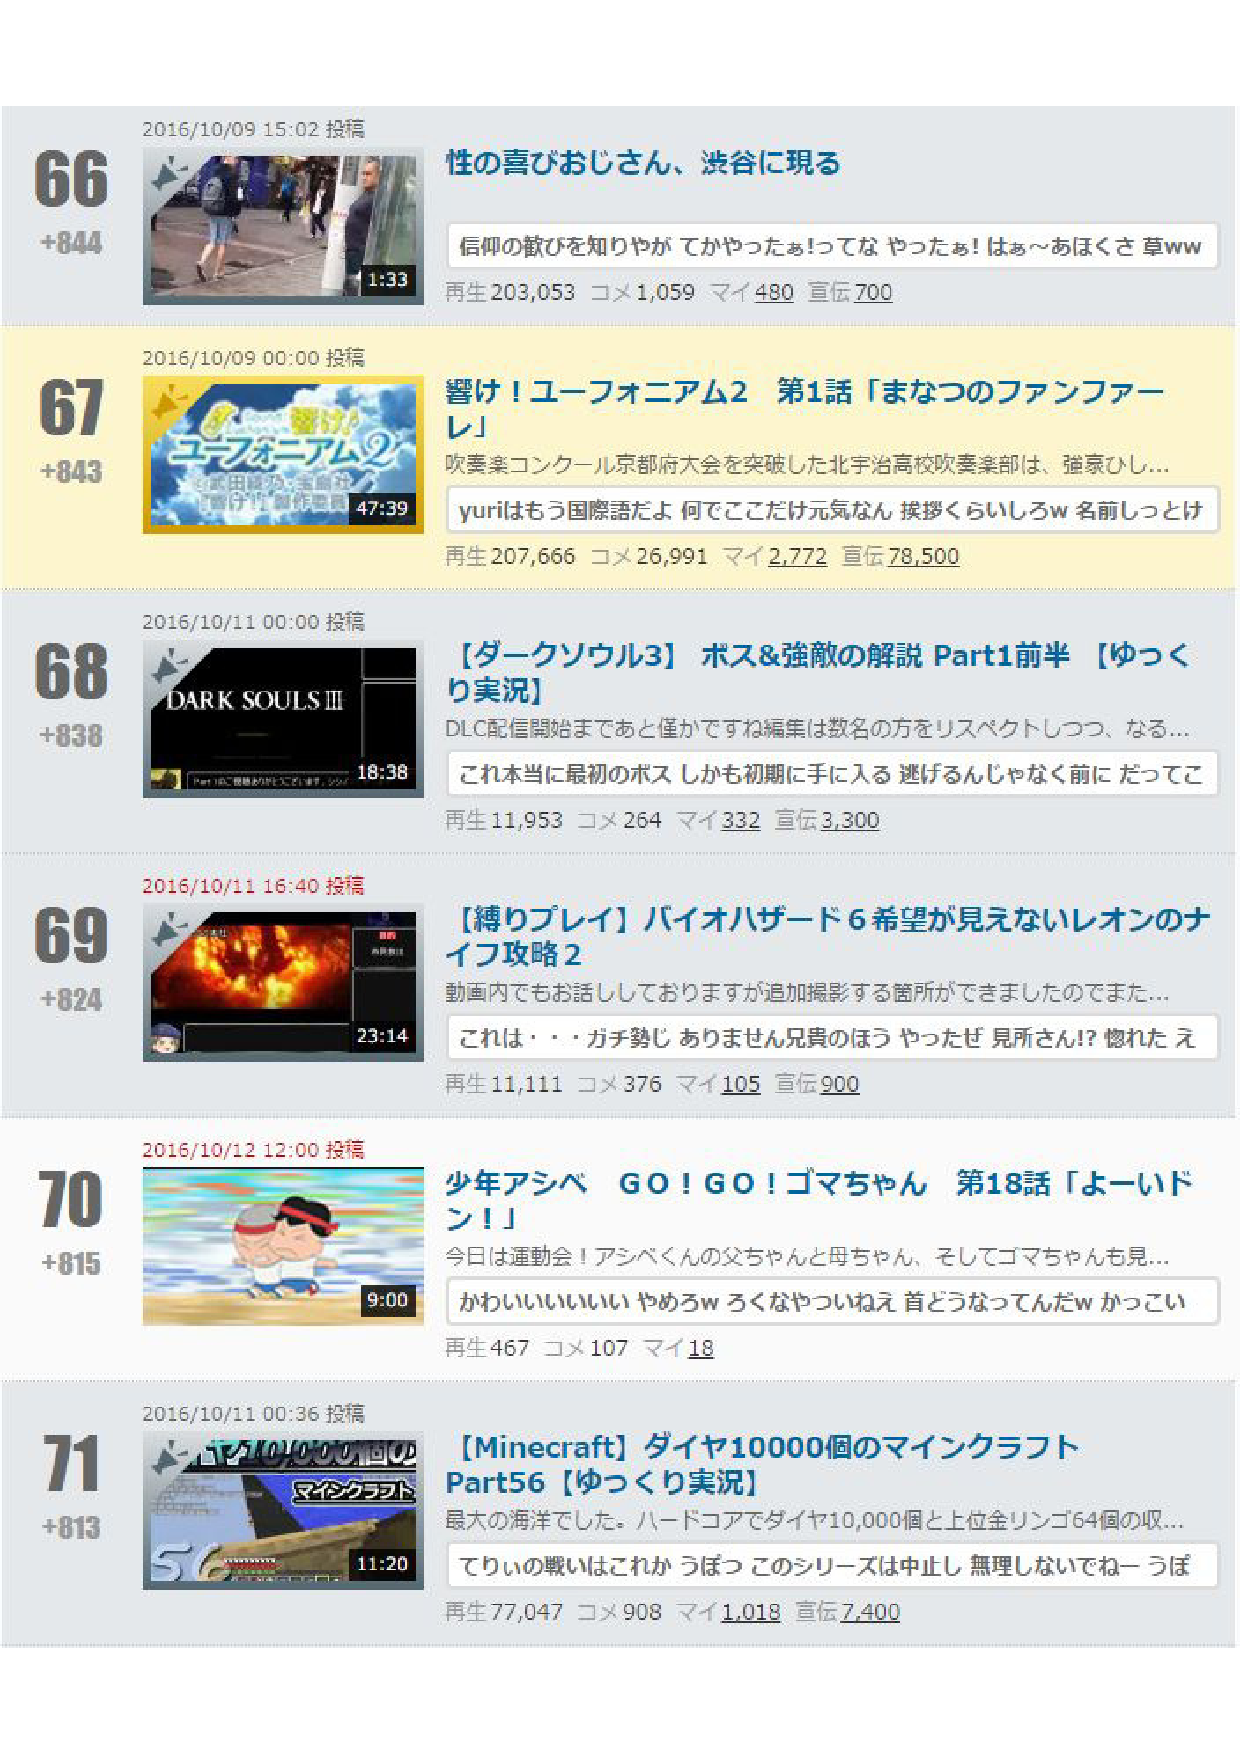
\includegraphics[width=7cm]{r12.pdf}
\caption{カテゴリ合算毎時総合ランキング}\label{abf}
\end{figure}

\begin{figure}[htb]
\centering
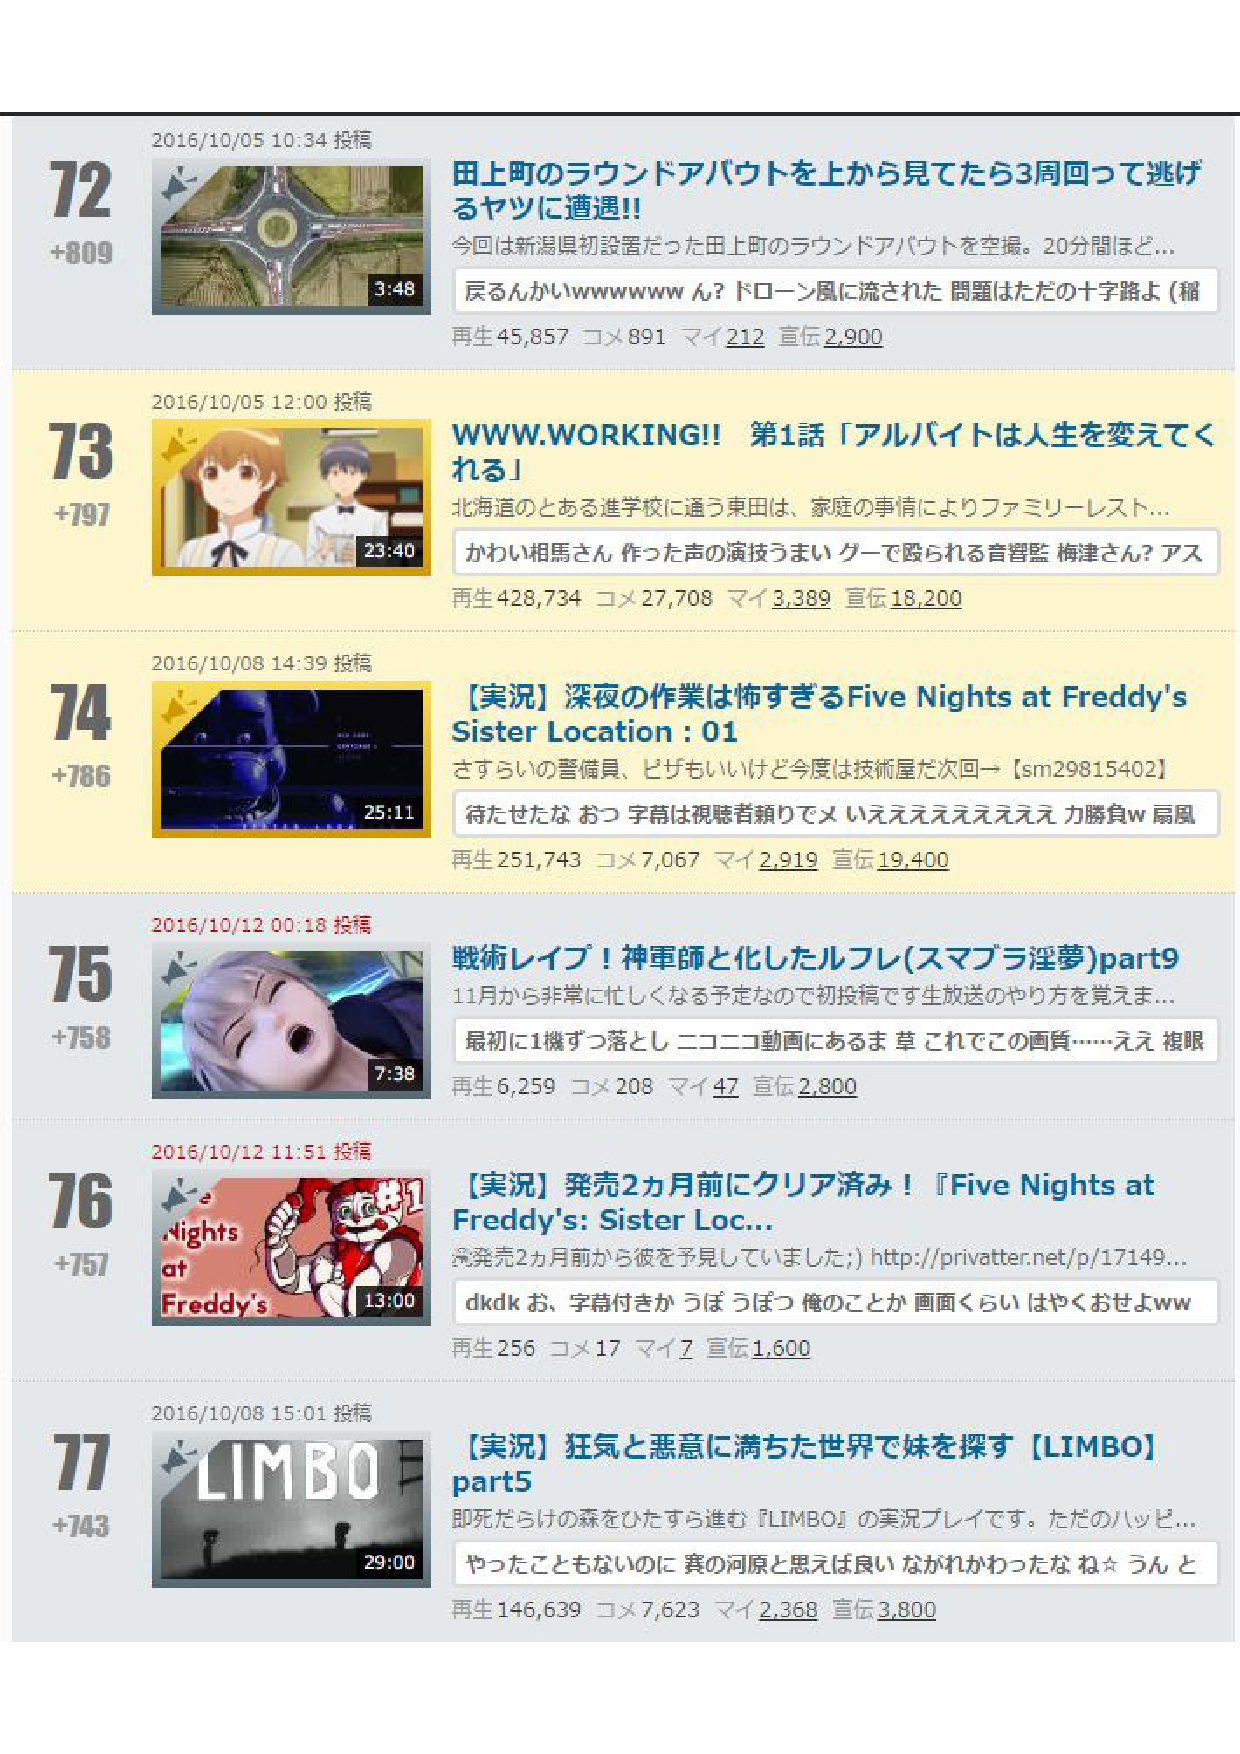
\includegraphics[width=7cm]{r13.pdf}
\caption{カテゴリ合算毎時総合ランキング}\label{aca}
\end{figure}

\begin{figure}[htb]
\centering
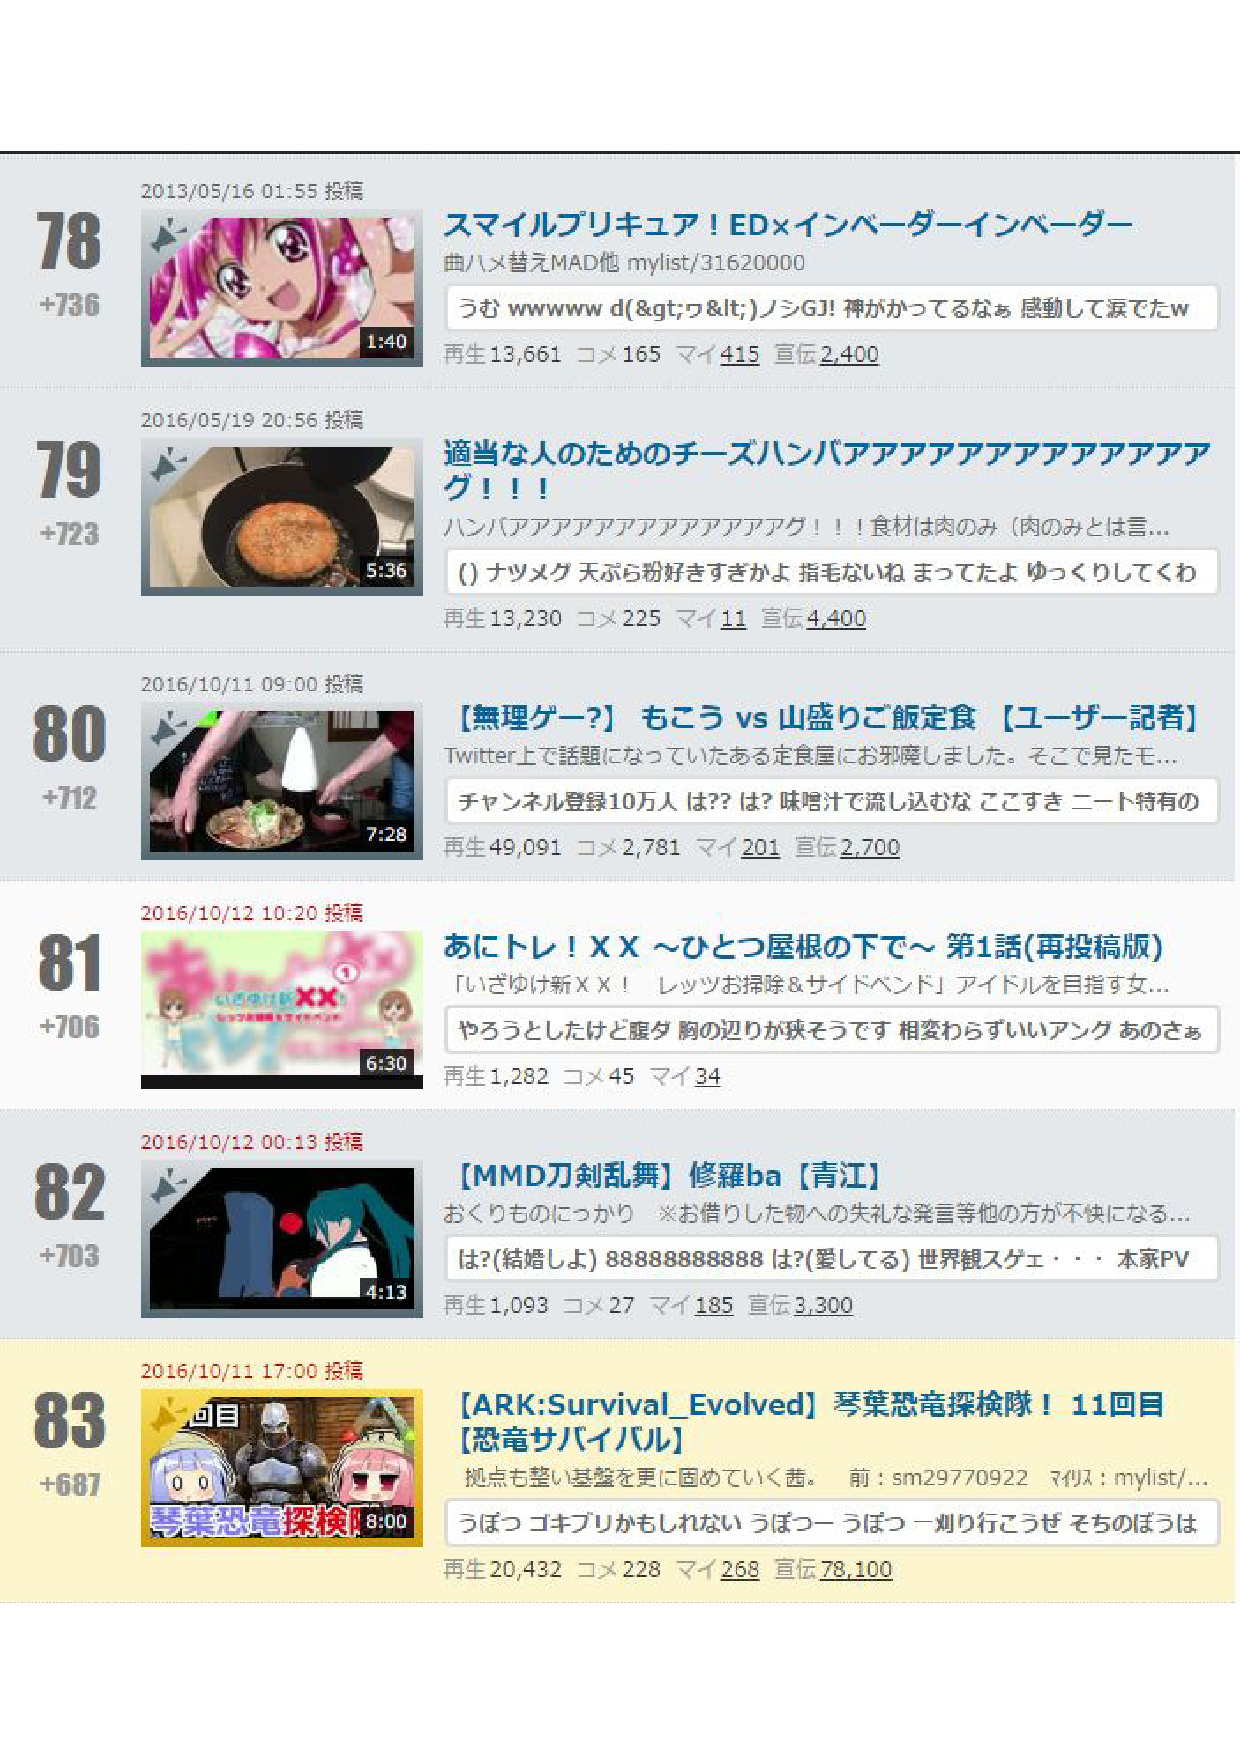
\includegraphics[width=7cm]{r14.pdf}
\caption{カテゴリ合算毎時総合ランキング}\label{acb}
\end{figure}

\begin{figure}[htb]
\centering
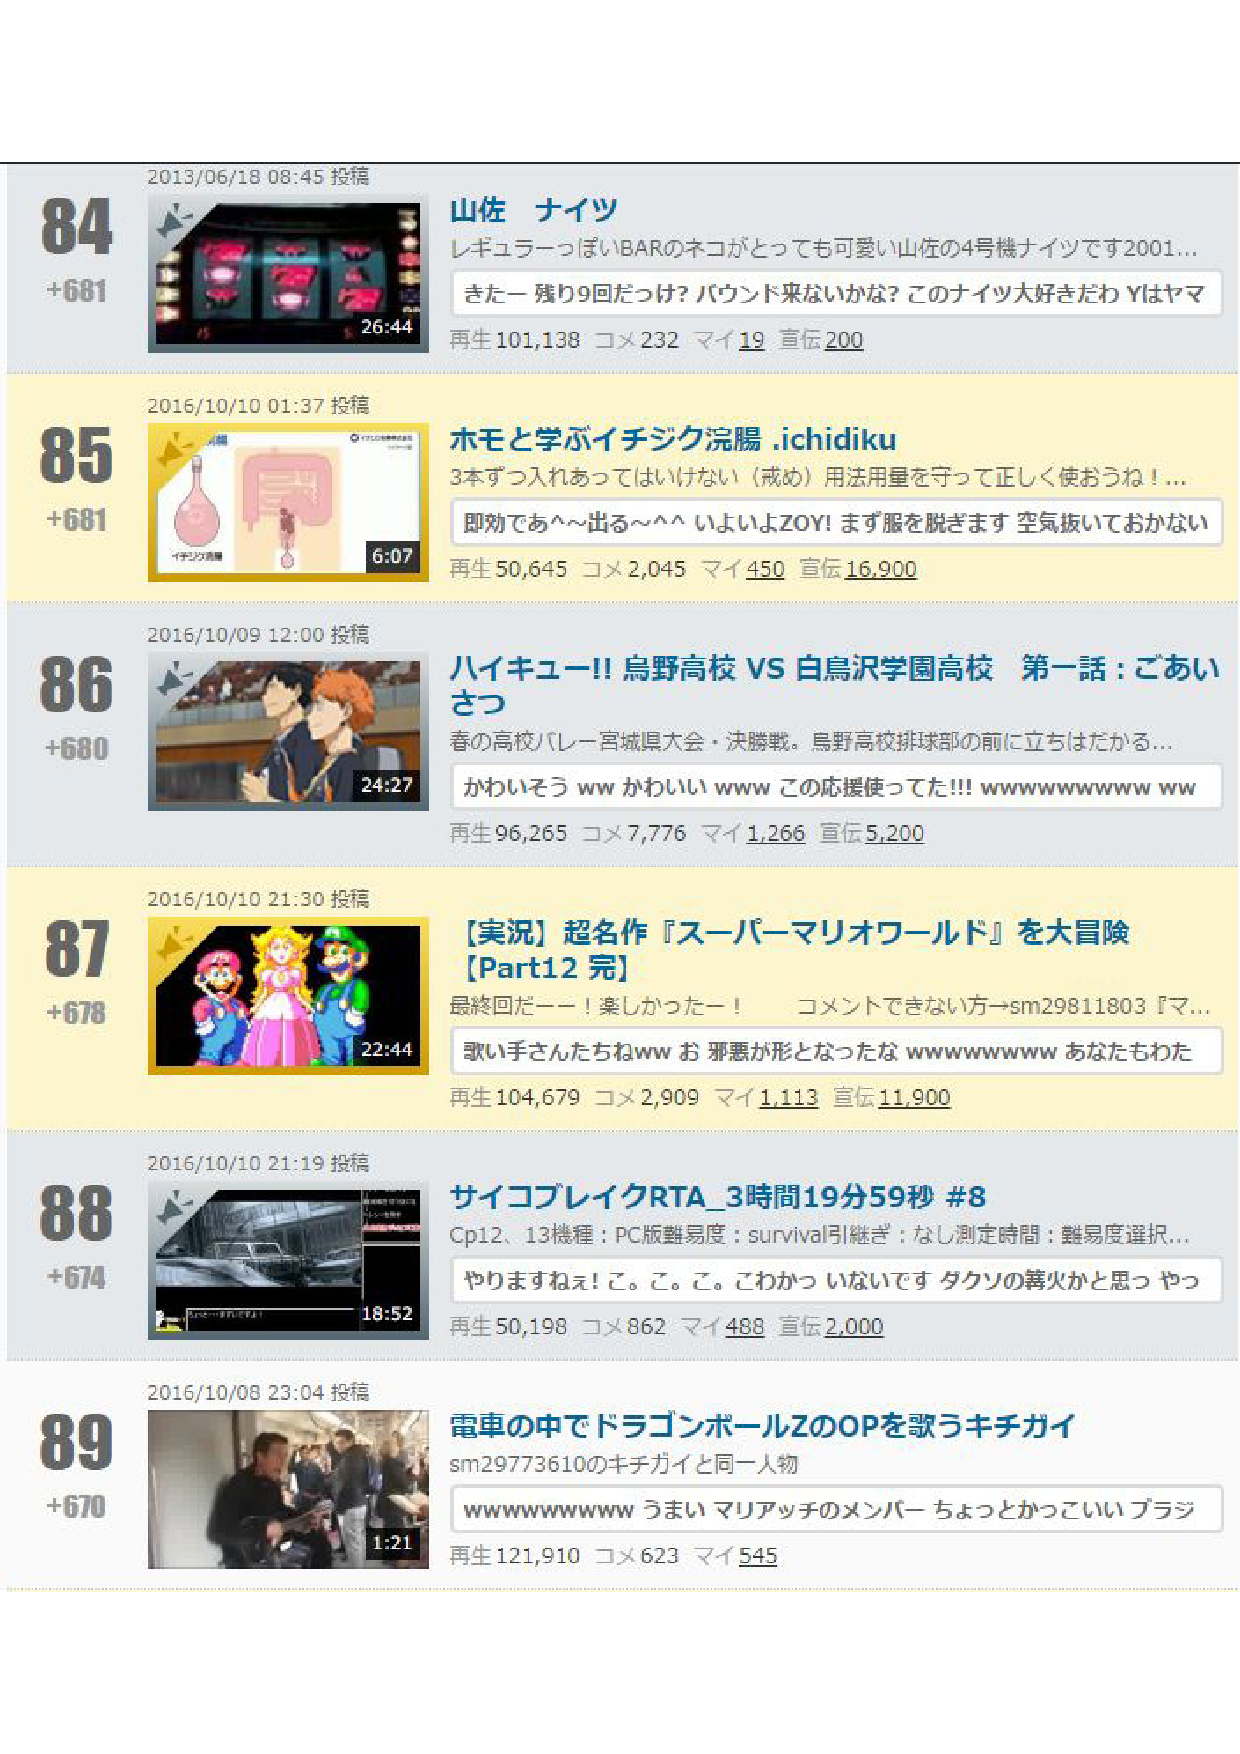
\includegraphics[width=7cm]{r15.pdf}
\caption{カテゴリ合算毎時総合ランキング}\label{acc}
\end{figure}

\begin{figure}[htb]
\centering
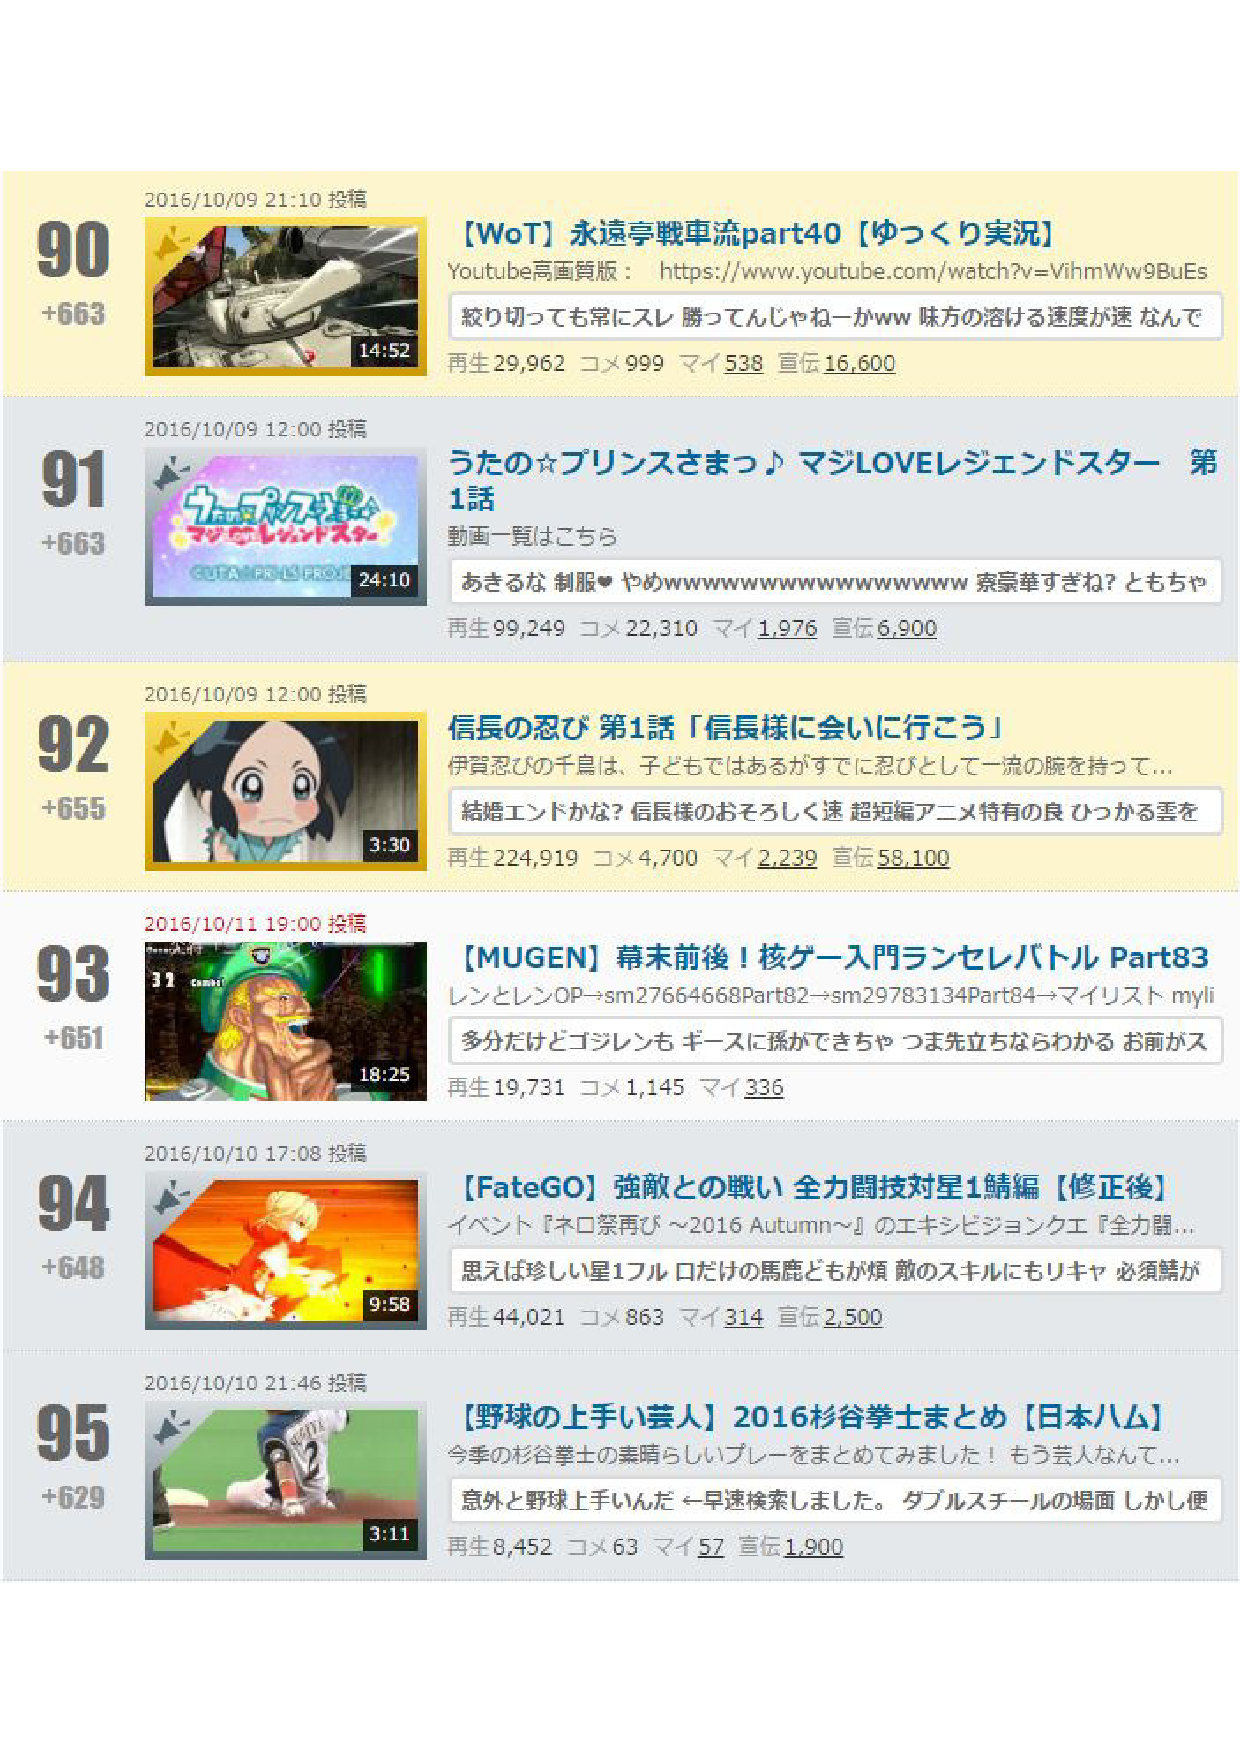
\includegraphics[width=7cm]{r16.pdf}
\caption{カテゴリ合算毎時総合ランキング}\label{acd}
\end{figure}

\begin{figure}[htb]
\centering
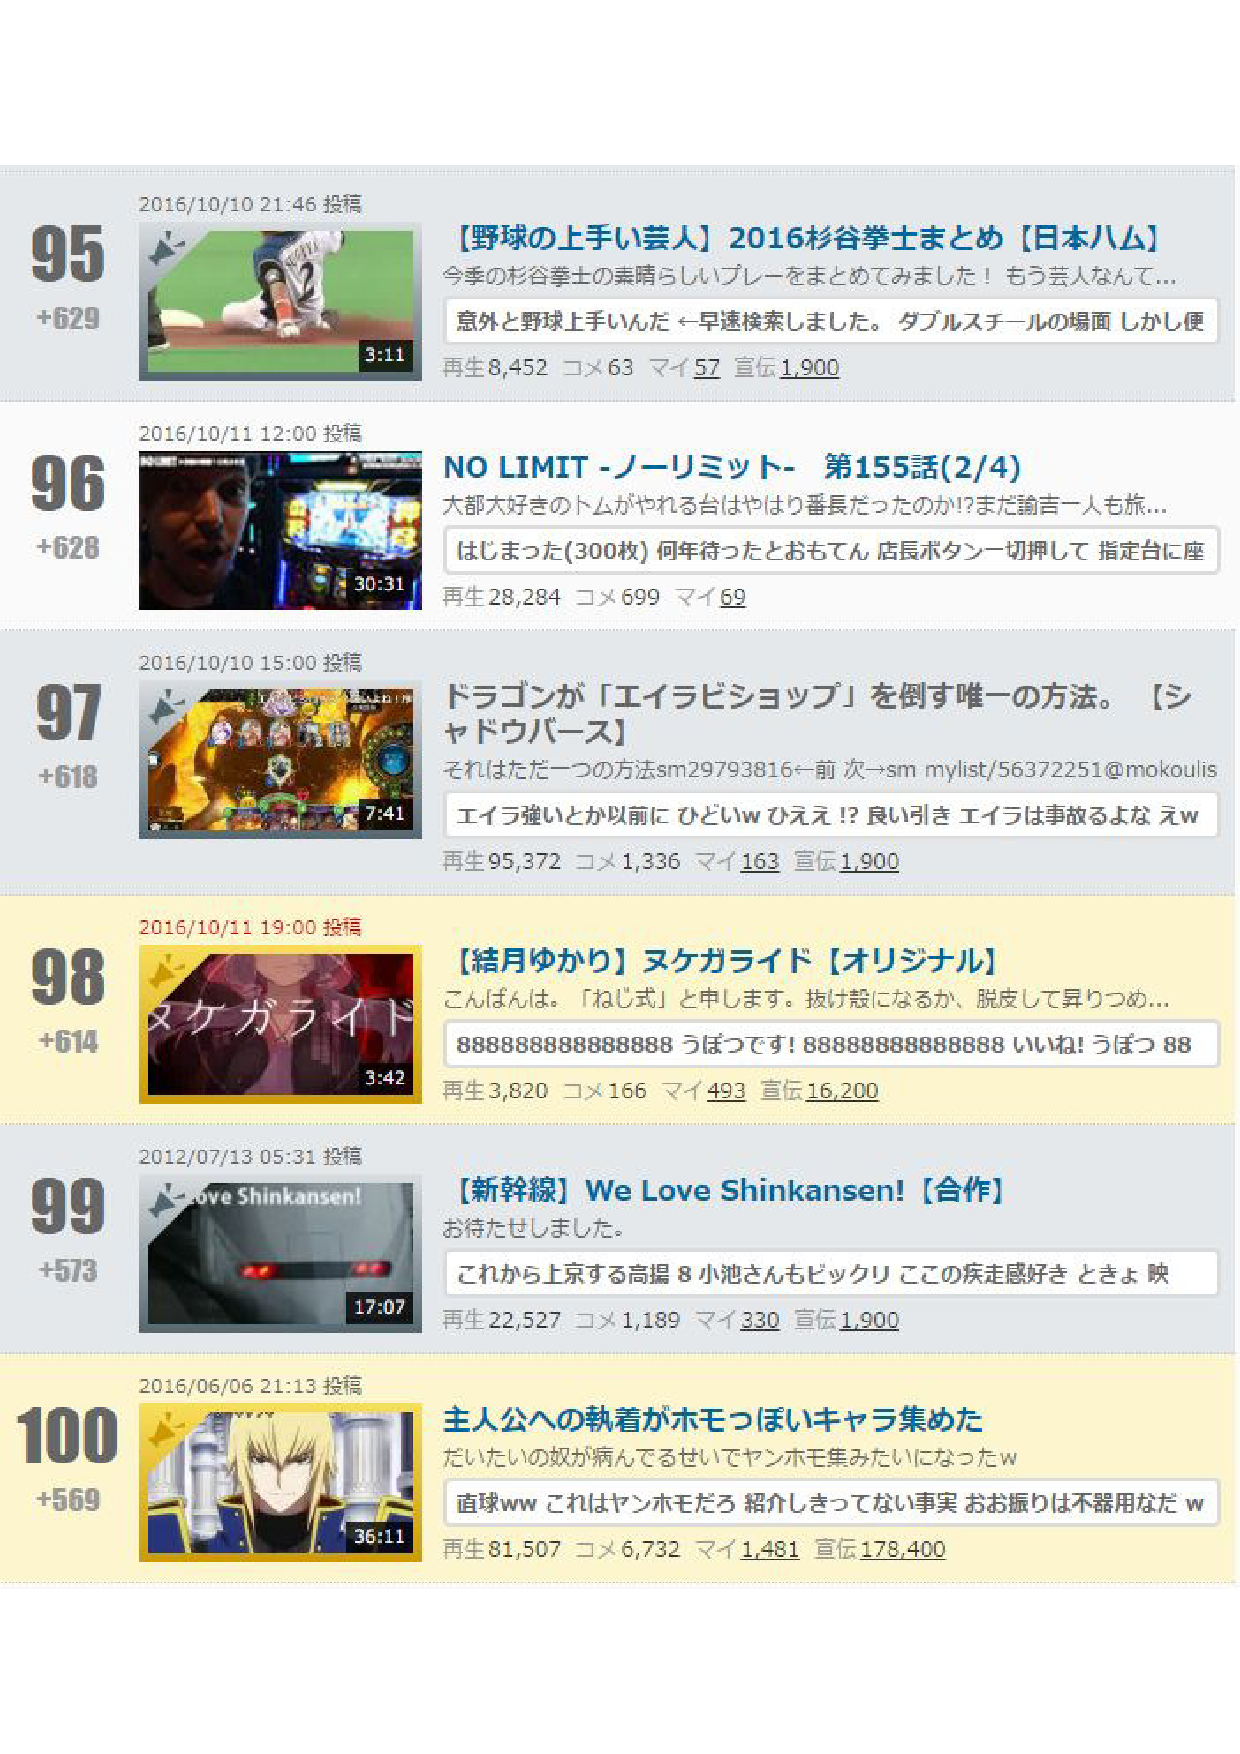
\includegraphics[width=7cm]{r17.pdf}
\caption{カテゴリ合算毎時総合ランキング}\label{ace}
\end{figure}

\clearpage


\section{ニコニコ動画ランキングAPIについて}
\subsubsection{APIについて}
APIとは,Application Programming Interfaceの略称で,あるコンピュータプログラムまたはソフトウェアの機能や管理するデータなどを,外部の他のプログラムから呼び出して利用するための手順やデータ形式などを定めた規約のことである.

\subsubsection{ニコニコ動画APIについて}
ニコニコ動画で利用可能なAPIである.


\section{ニコニコ動画ランキングAPIの導入}

\subsubsection{ニコニコ動画ランキングAPIについて}
本研究で使用したAPIは「ニコ動のランキング情報をJSONで取得してみる - yutaponのブログ」\cite{nikoapi}を使用したものである.本研究で使用したAPIはニコニコ動画にあるランキングからニコニコ動画に投稿されている動画の動画IDを取得し,その動画IDをもとに動画の詳細情報を取得するものである.実行環境がnode.jsのためXMLの取り扱いが難しい.そのためxmljsonというモジュールを使用しXMLをSONに変更する.

\subsubsection{xmljsonの導入}
コマンドプロプトで作業ディレクトリに移動し,インストールを行う.

コマンドは以下の通りである.
	\begin{verbatim}
			$ cd path/to/workspace
			$ express -c stylus project_name
			$ cd project_name && npm install
			$ npm install --save xmljson
	\end{verbatim}

補足として,ここで作られるworkspaceの名前を変更してもよい.

例  cd path/to/nico

\subsubsection{ニコニコ動画のランキングの取得}
コマンドプロプトでモジュールのインストールを行う.

コマンドは
	\begin{verbatim}
			$ npm install --save async underscore http xmljson
	\end{verbatim}
である.

次に,nico.jsを作成し,この中にモジュールのコードを書いていく.

コードは以下の通りである.


	\begin{figure}[h]
		\centering
		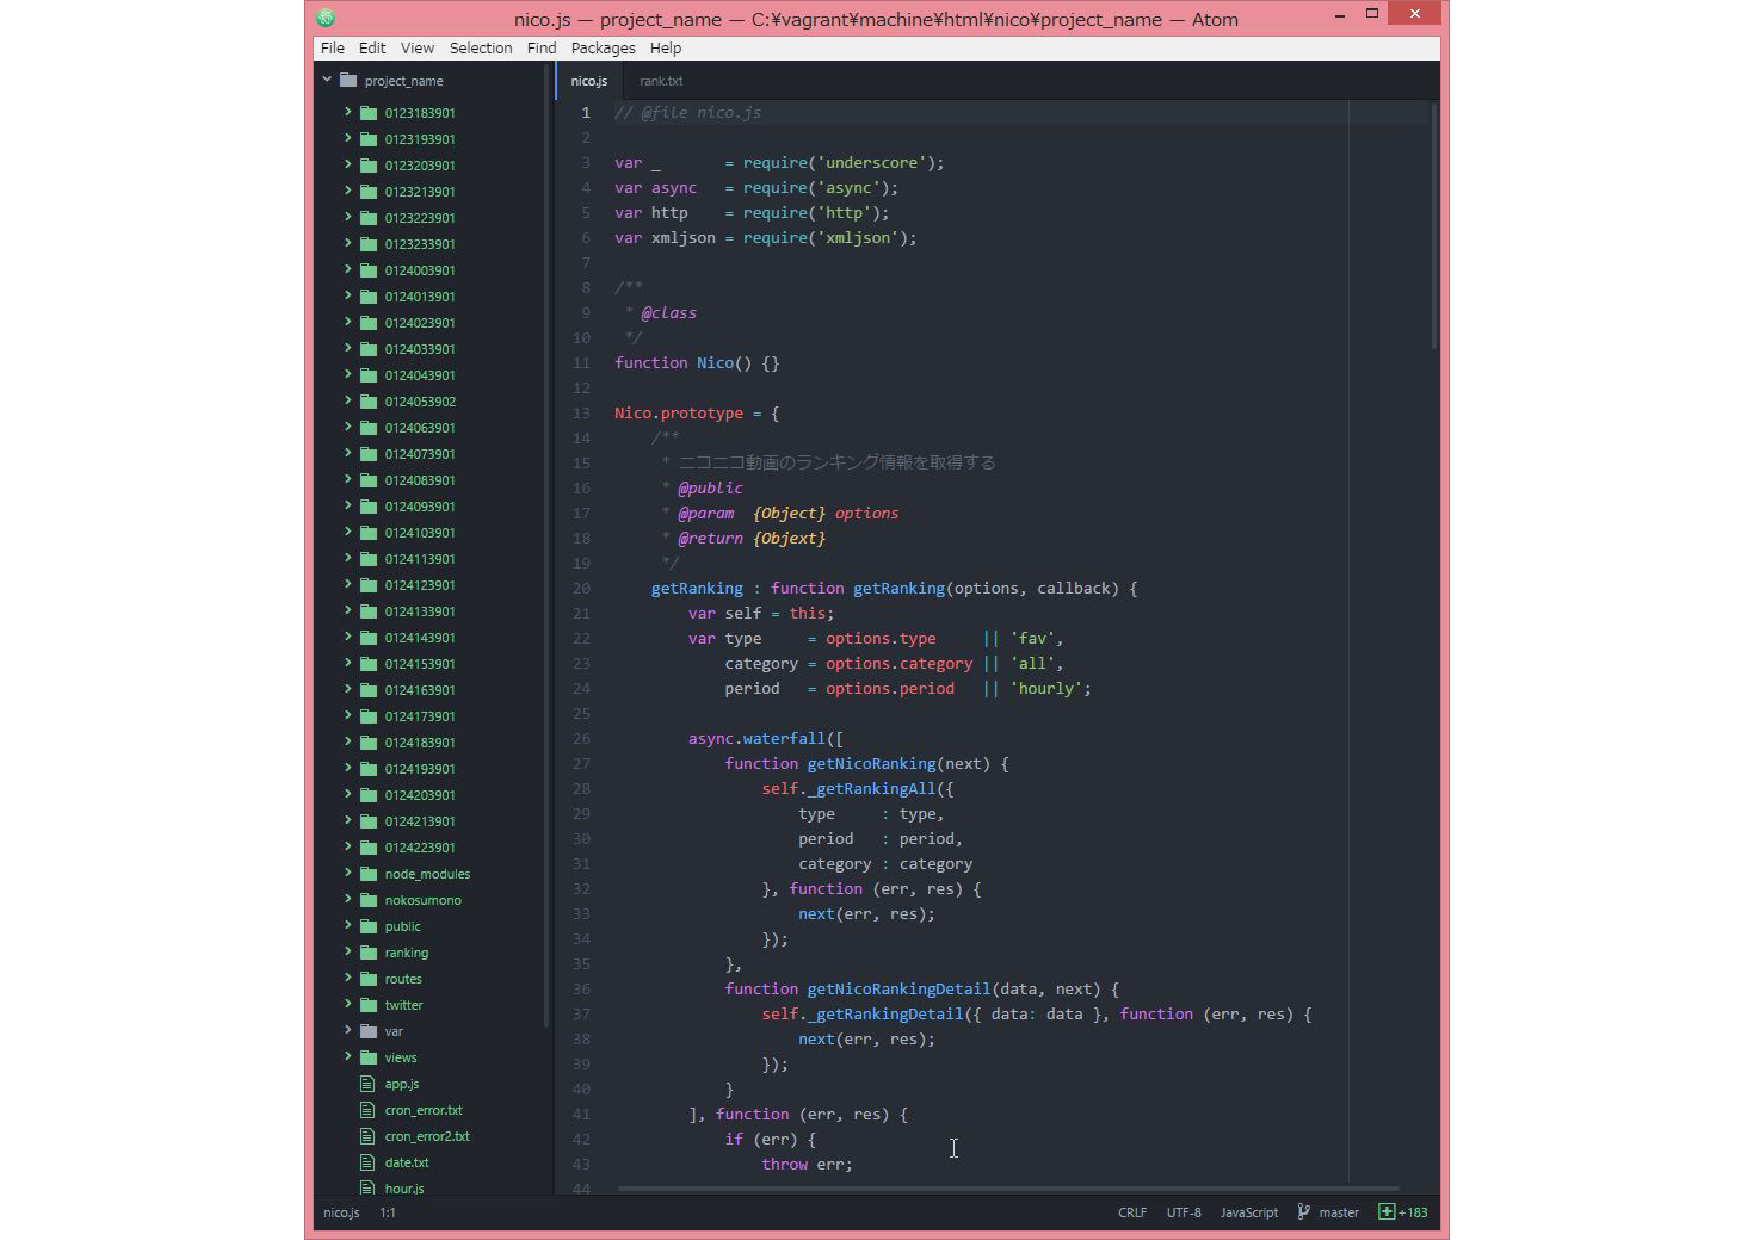
\includegraphics[width=14cm]{nico01.pdf}
		\caption{nico.js01}\label{ace}
	\end{figure}


	\begin{figure}[h]
		\centering
		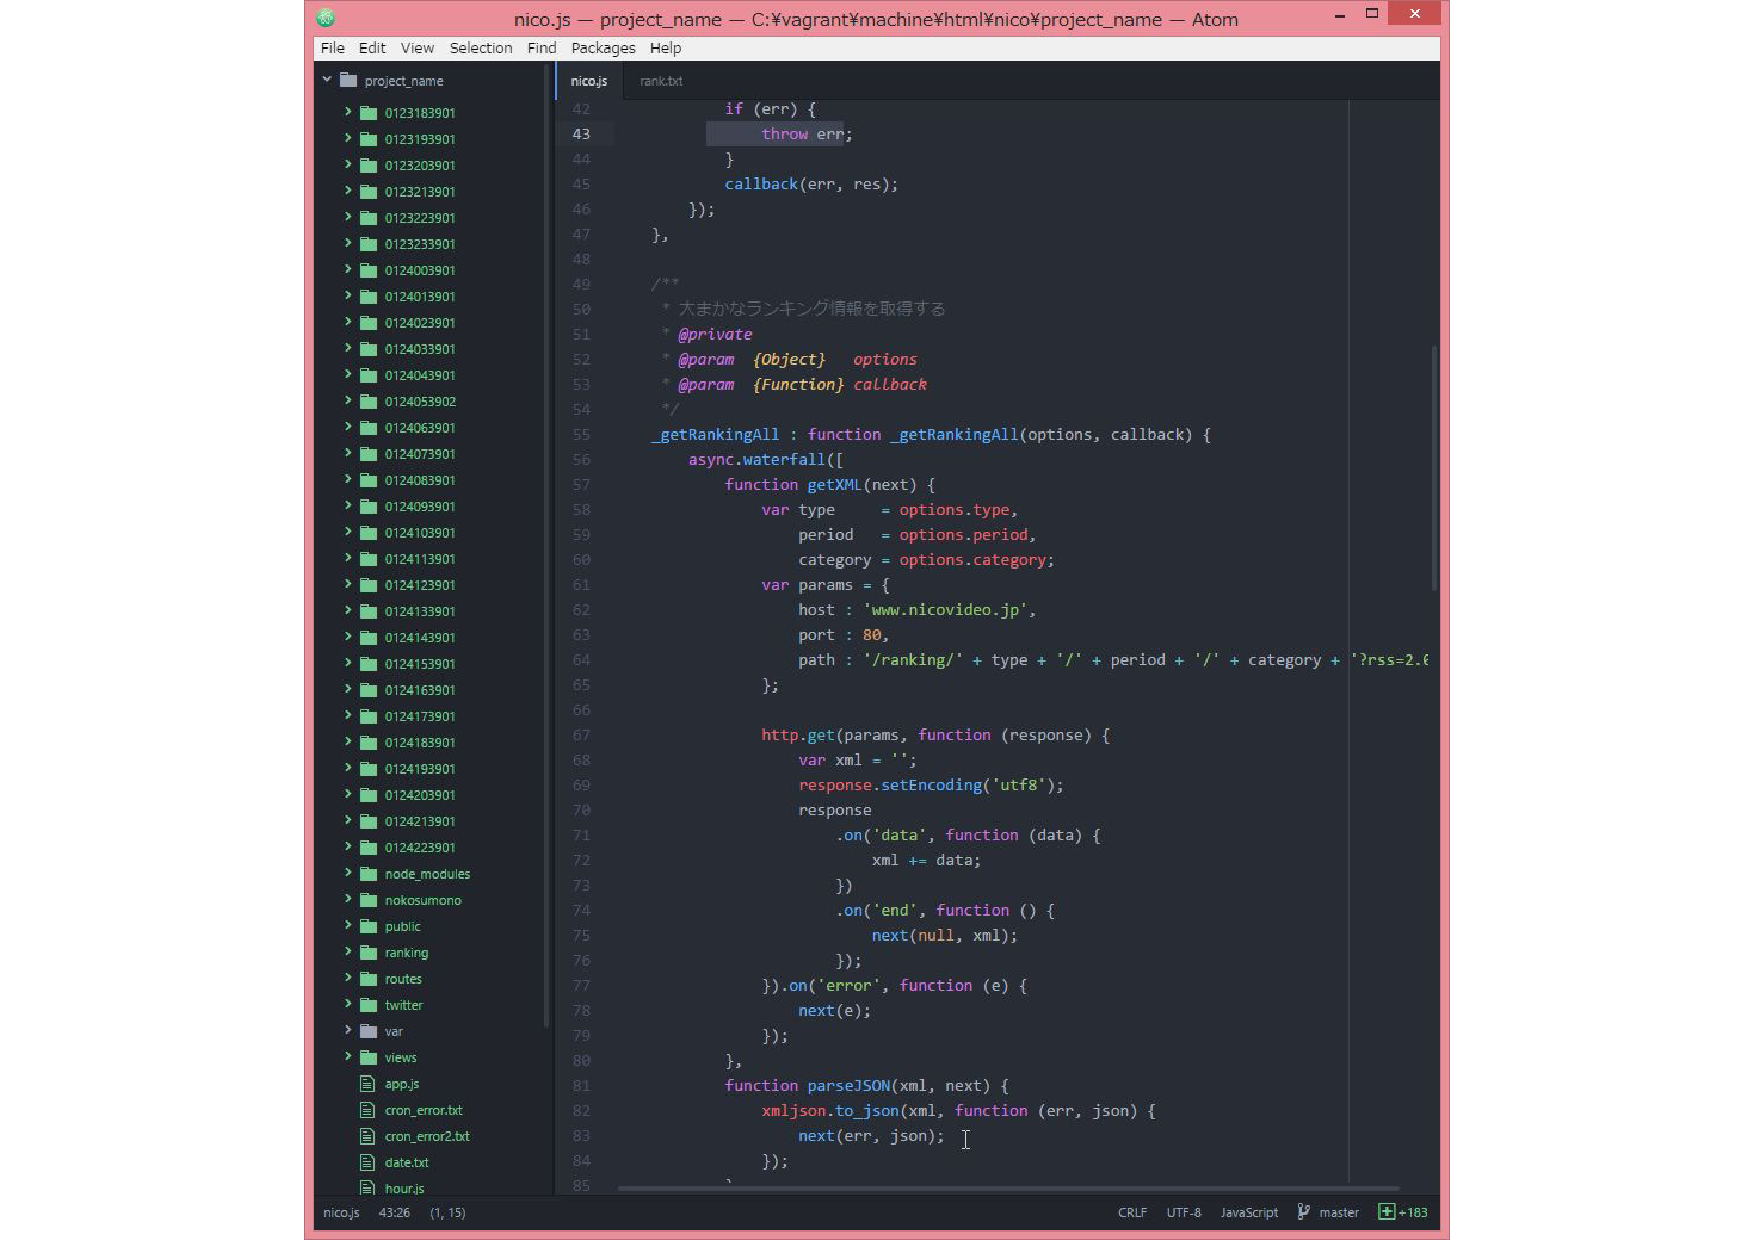
\includegraphics[width=14cm]{nico02.pdf}
		\caption{nico.js02}\label{ace}
	\end{figure}


	\begin{figure}[h]
		\centering
		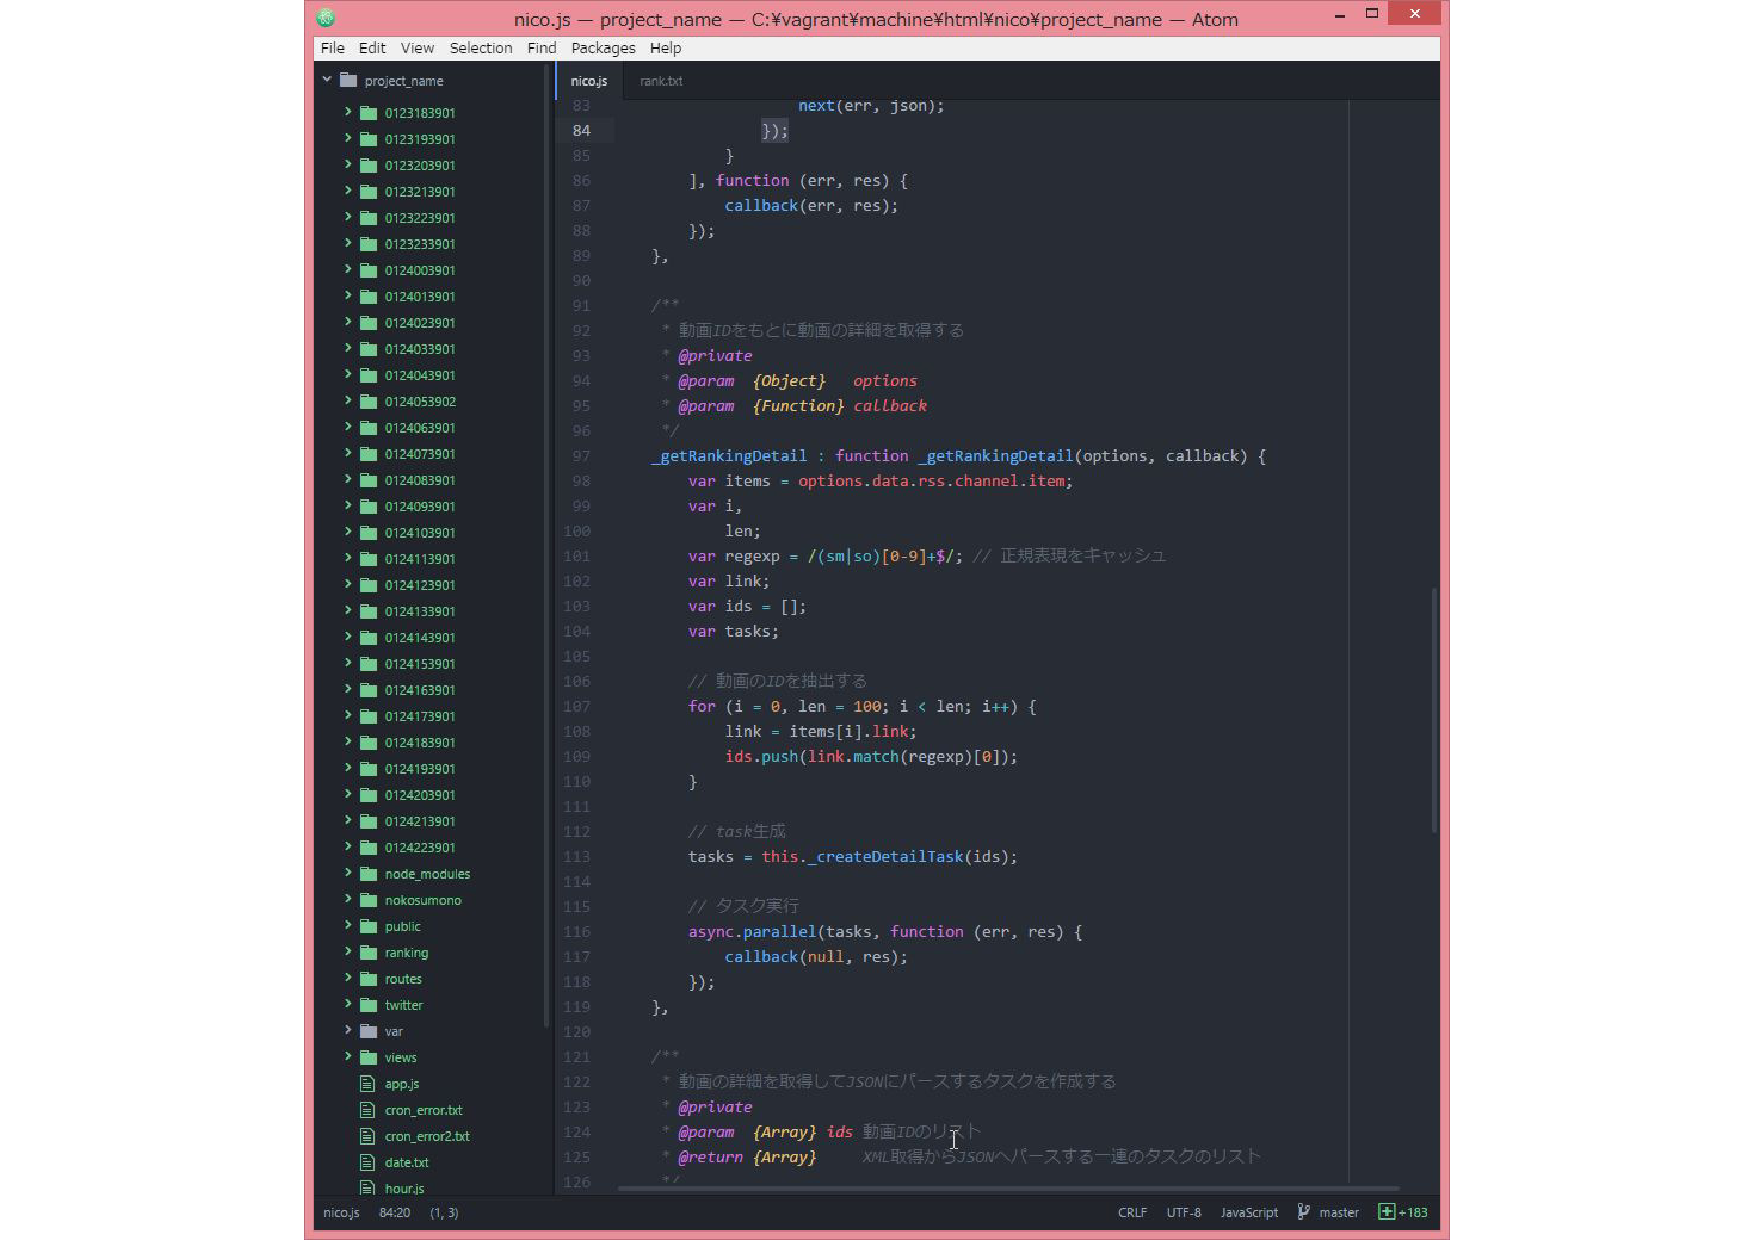
\includegraphics[width=14cm]{nico03.pdf}
		\caption{nico.js03}\label{ace}
	\end{figure}

	\begin{figure}[h]
		\centering
		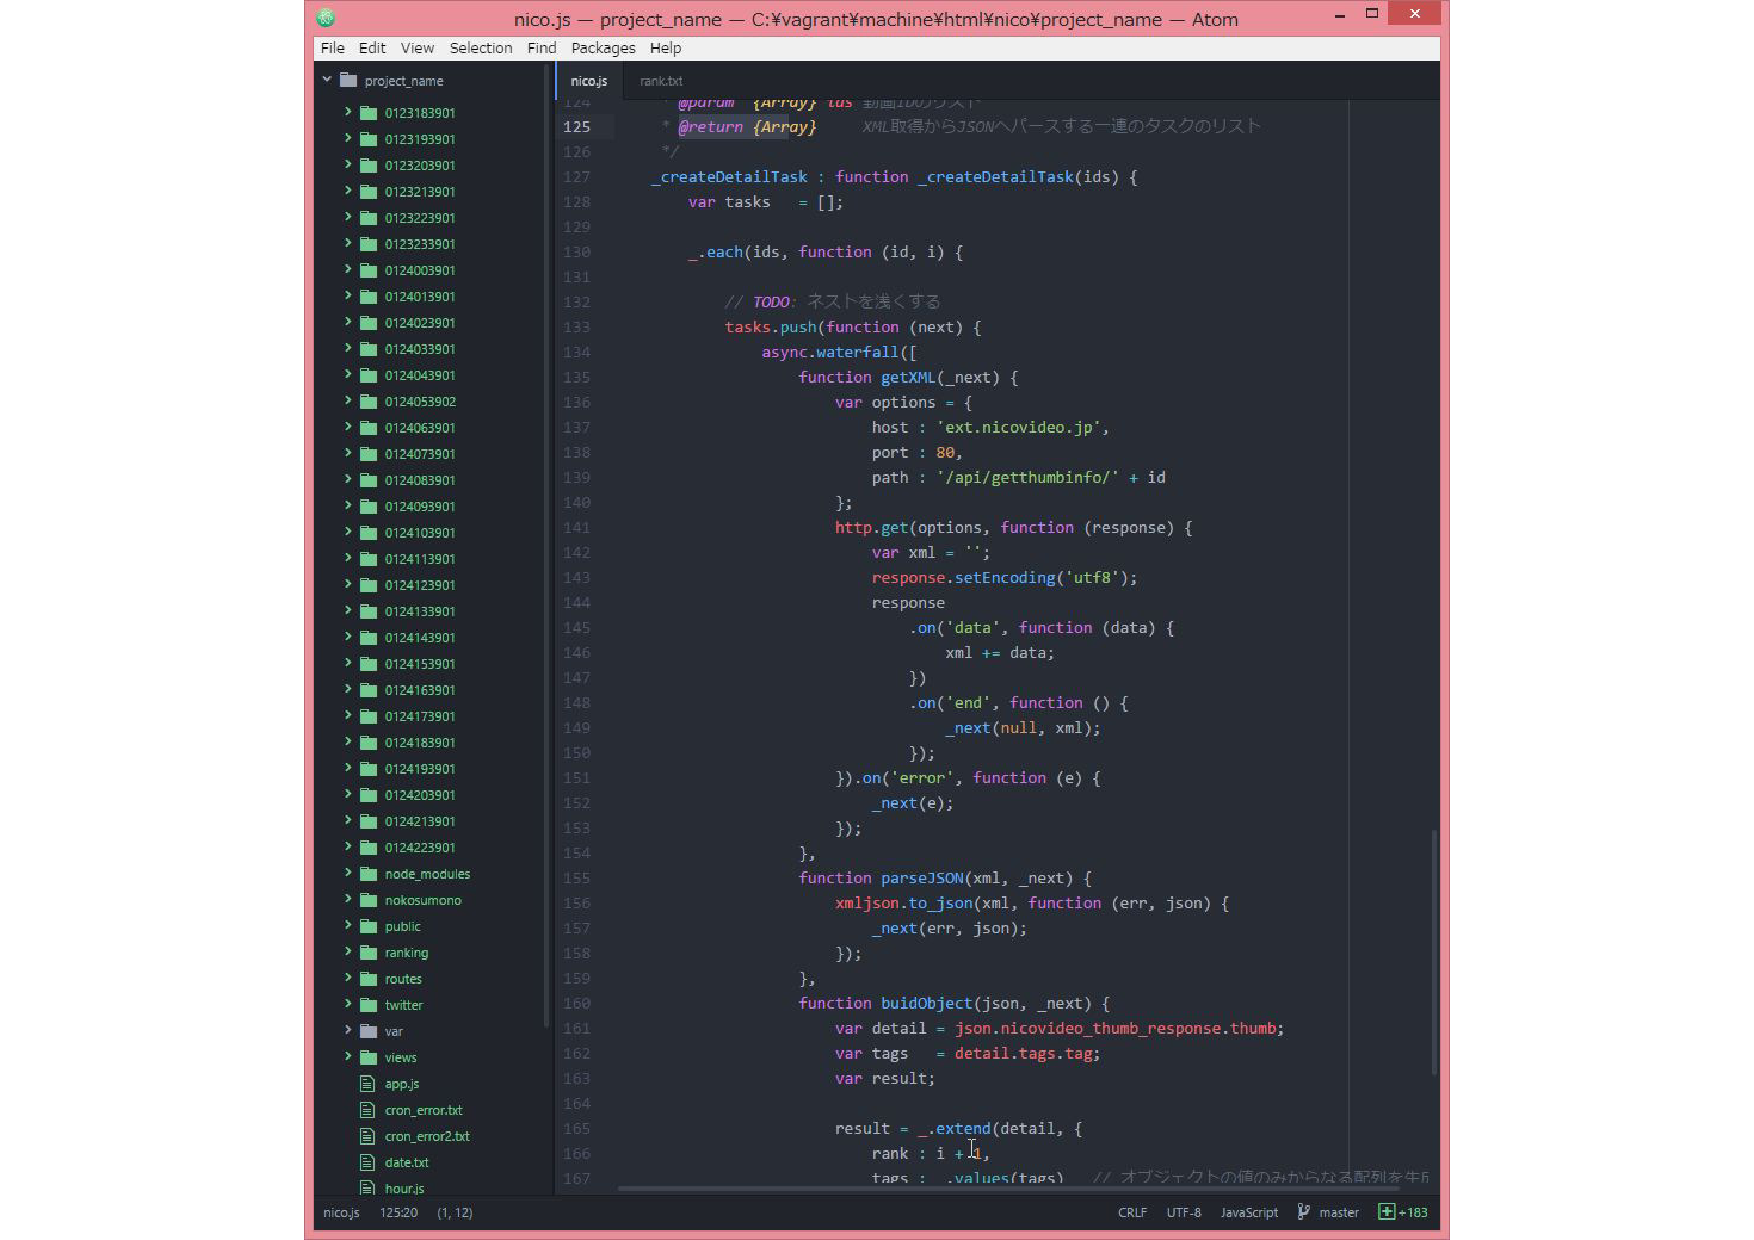
\includegraphics[width=14cm]{nico04.pdf}
		\caption{nico.js04}\label{ace}
	\end{figure}

	\begin{figure}[h]
		\centering
		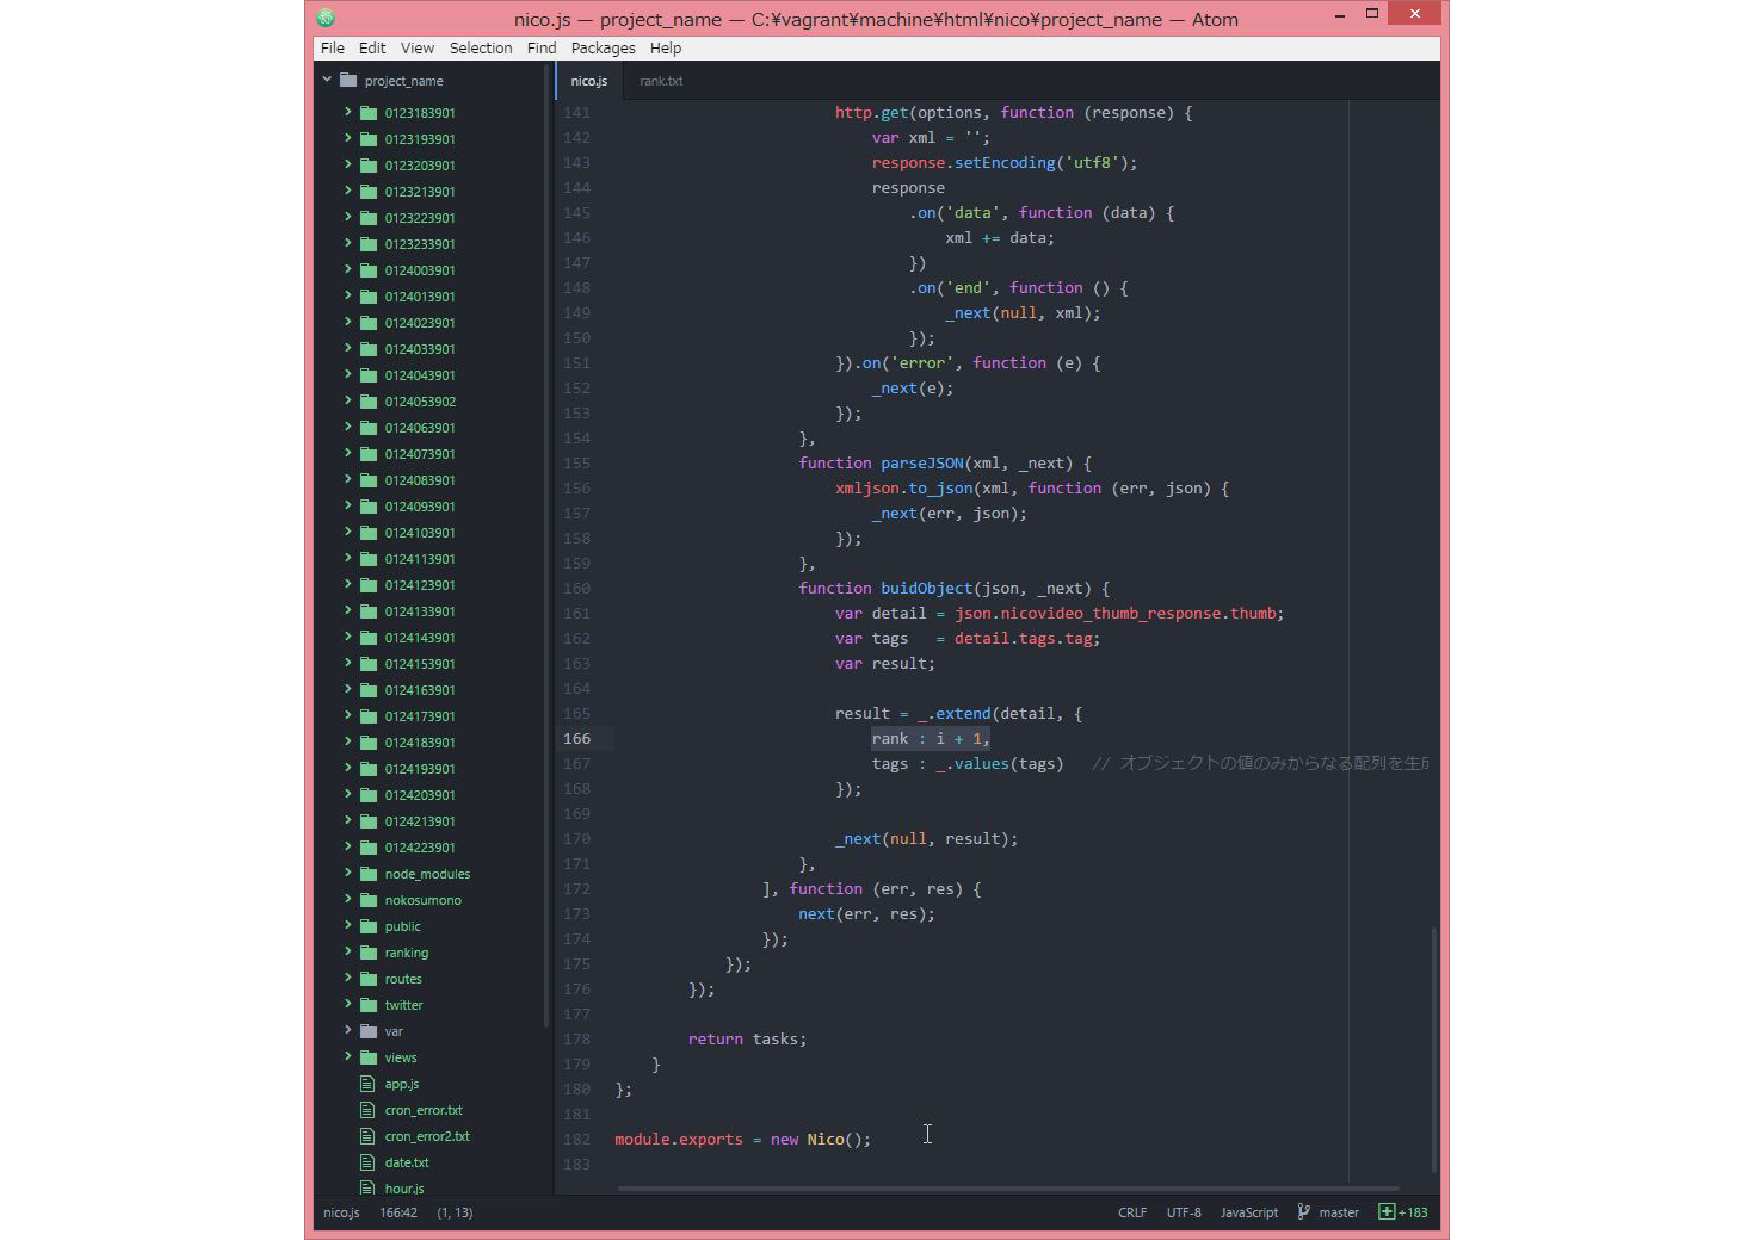
\includegraphics[width=14cm]{nico05.pdf}
		\caption{nico.js05}\label{ace}
	\end{figure}

\clearpage

\subsection*{モジュールの呼び出し}
作ったモジュールを呼び出すために「kidou.js」を作成し,この中にコードを書いていく.

kidou.jsの内容は以下のとおりである.


	\begin{figure}[h]
		\centering
		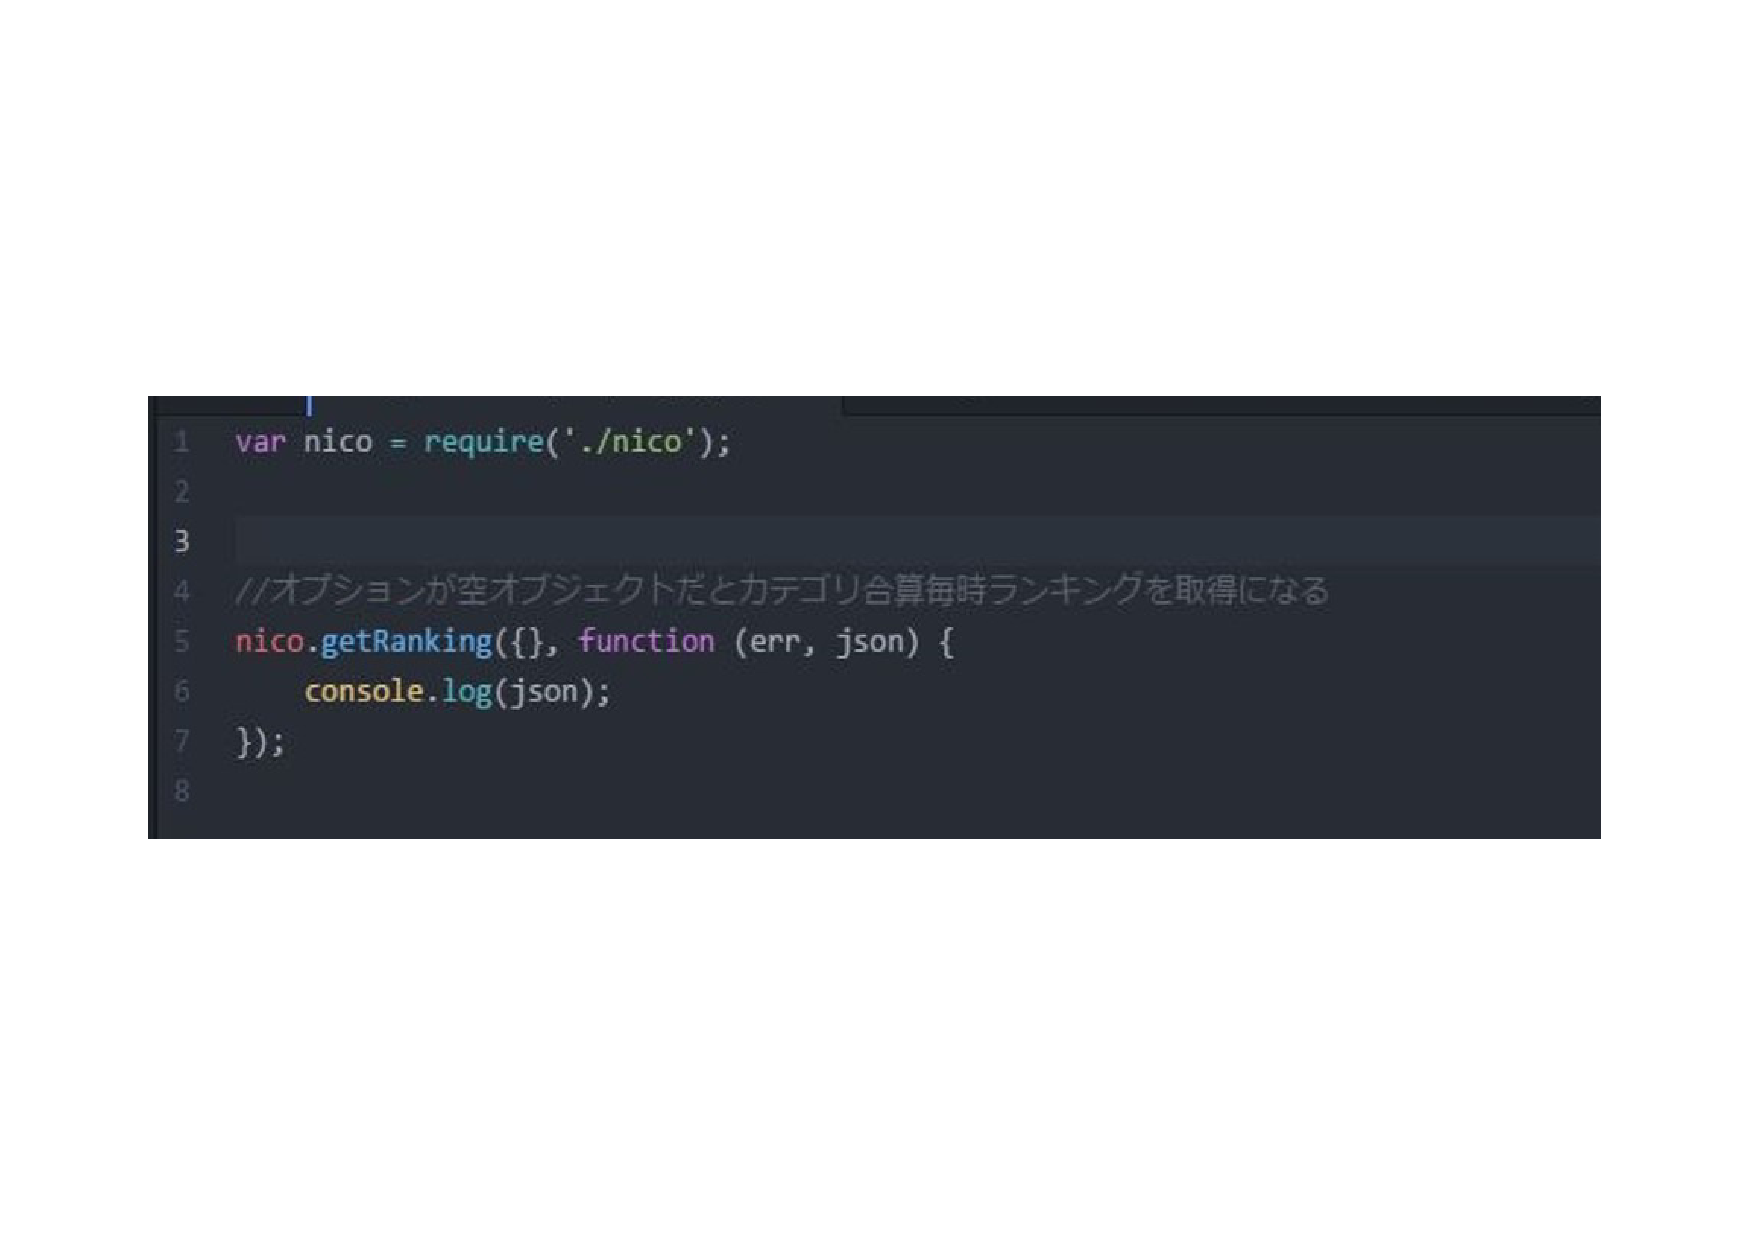
\includegraphics[width=14cm]{kidou.pdf}
		\caption{kidou.js}\label{ace}
	\end{figure}

\clearpage

kidou.jsをコマンドプロプトにnode kidou.jsを書き込み起動させると,起動させた時間のカテゴリ合算毎時総合ランキングの1位から100位までの動画の詳細情報を取得することが出来る.

取得したデータはこのように表示される.

	\begin{figure}[h]
		\centering
		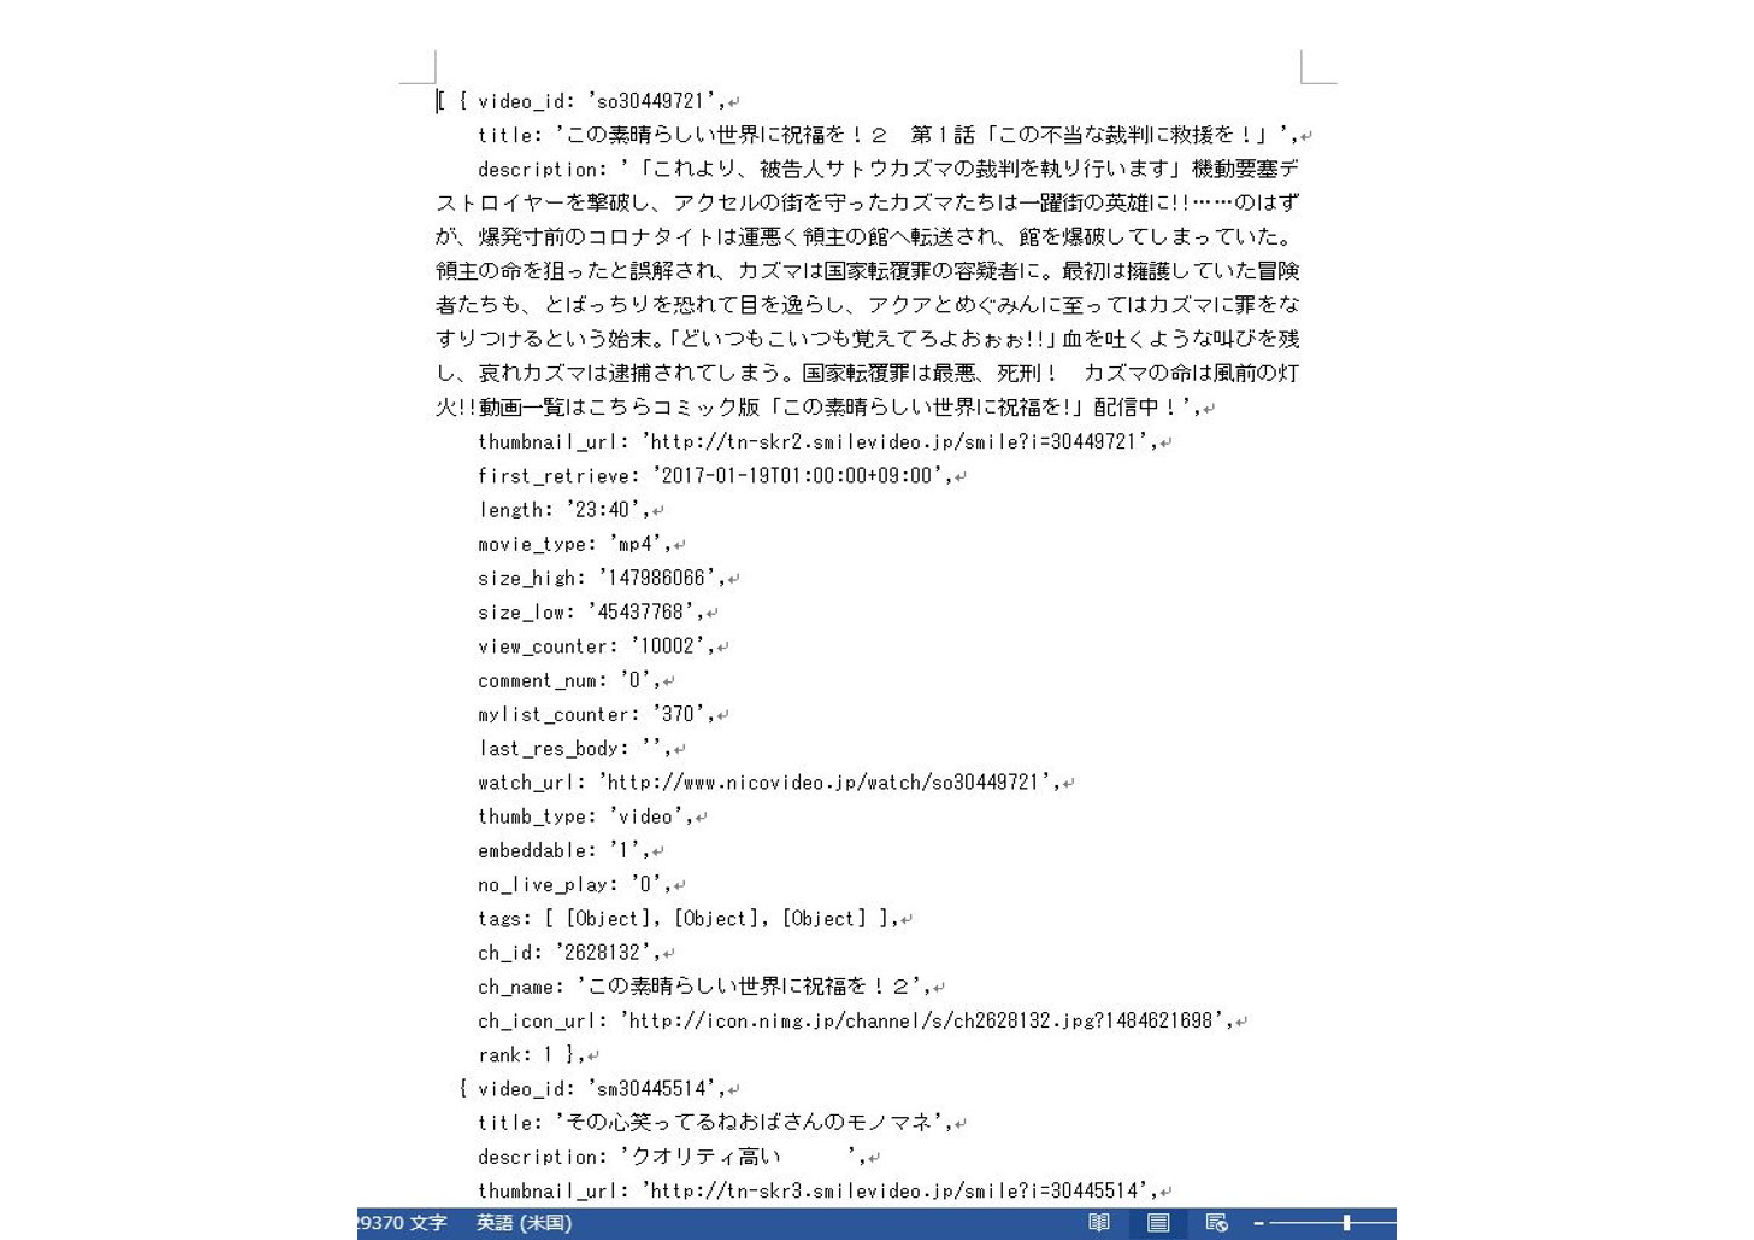
\includegraphics[width=14cm]{zyouhou.pdf}
		\caption{kidou.js}\label{ace}
	\end{figure}
    
    以降に2位から100位までの動画の詳細情報が書かれている.



以上が,本研究においてニコニコ動画ランキングAPIからのランキングと動画の詳細情報データの取集方法である.

\clearpage
\chapter{Twitterについて}



\section{本章の構成}

本章では本研究で使用するTwitterについて記す.


\section{Twitterとは}
Twitterは,「ツイート」と称される140文字以内の短文の投稿を共有するウェブ上の情報サービスである.

	\begin{figure}[h]
		\centering
		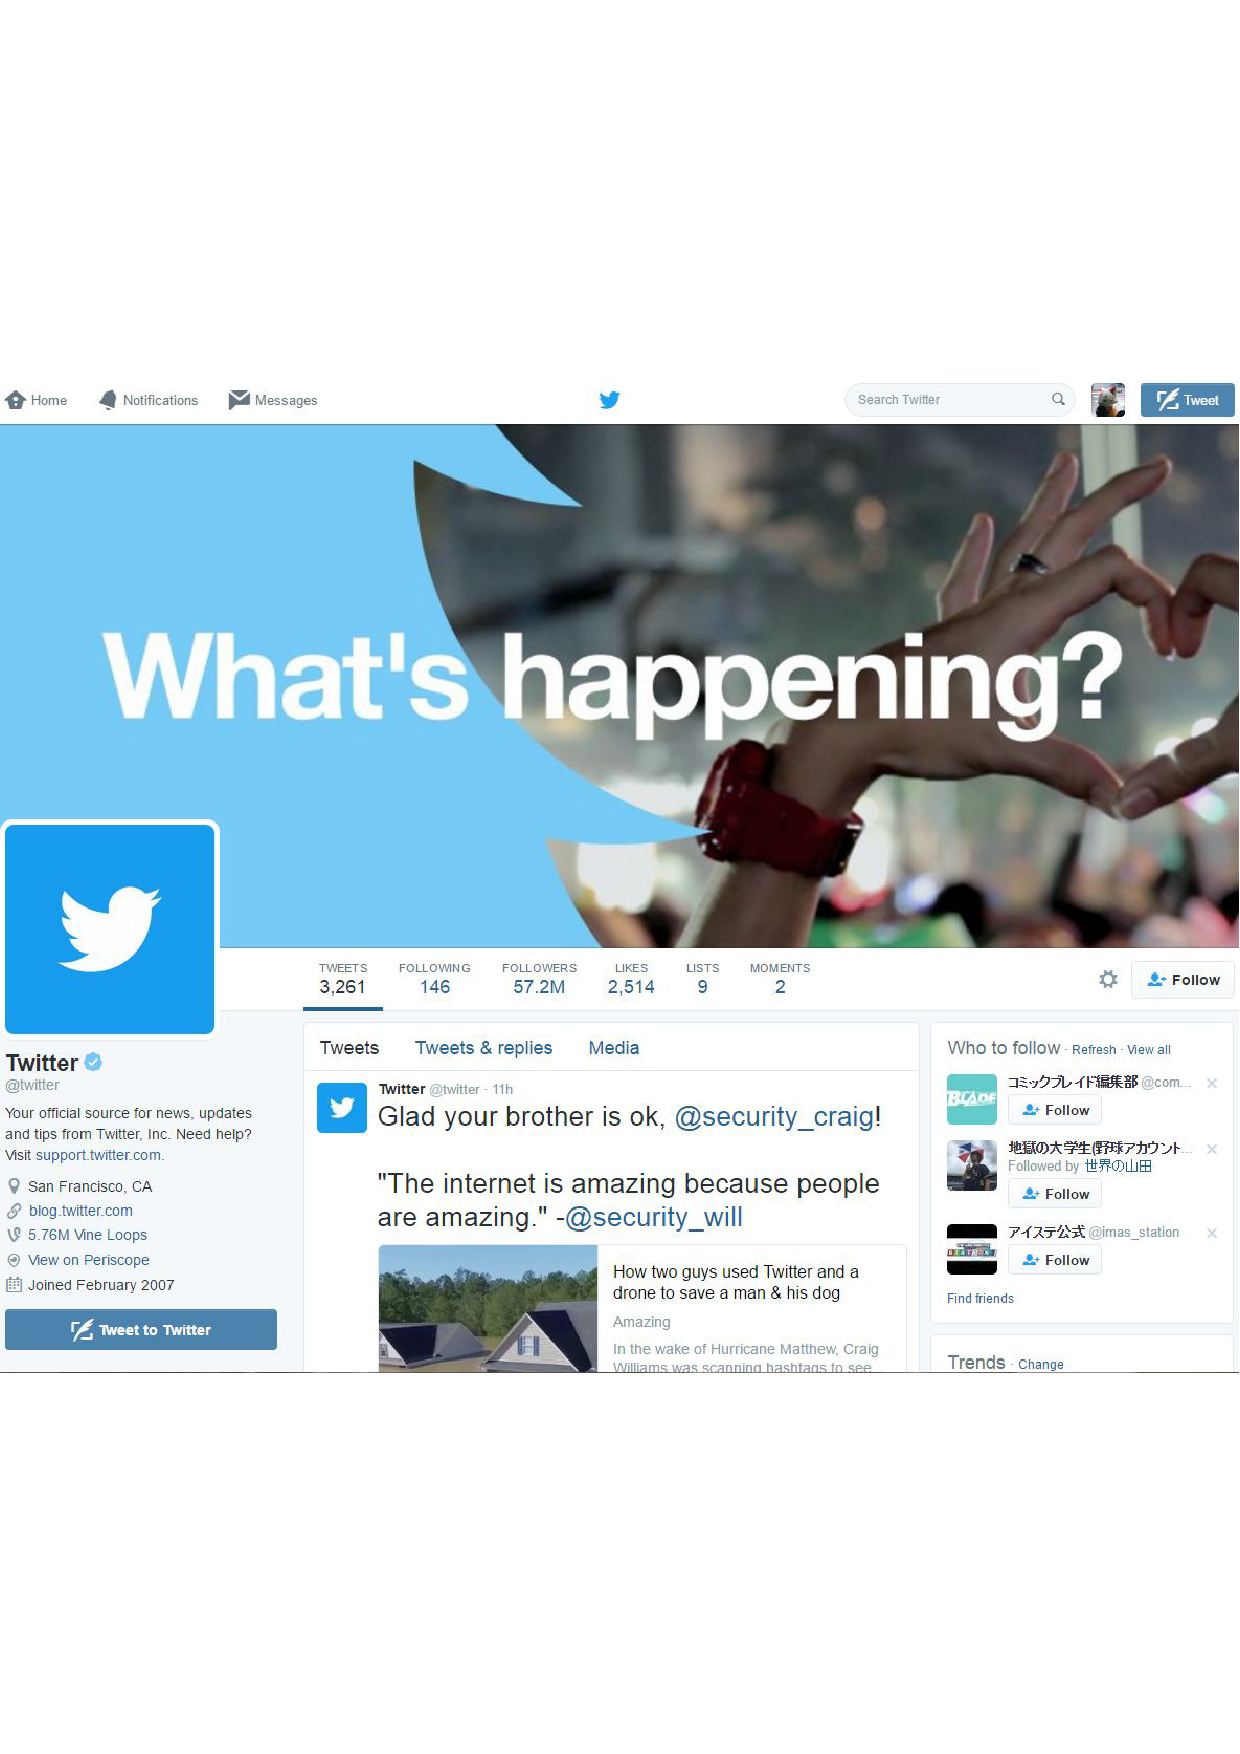
\includegraphics[width=10cm]{twi.pdf}
		\caption{Twitterのホームページ}\label{ace}
	\end{figure}


\clearpage
\section{用語}
Twitterで使用する用語に関して解説する.

\subsubsection*{ツイート}
140文字以下の文字列のこと.つぶやきと呼ばれる.
\begin{figure}[htb]
\centering
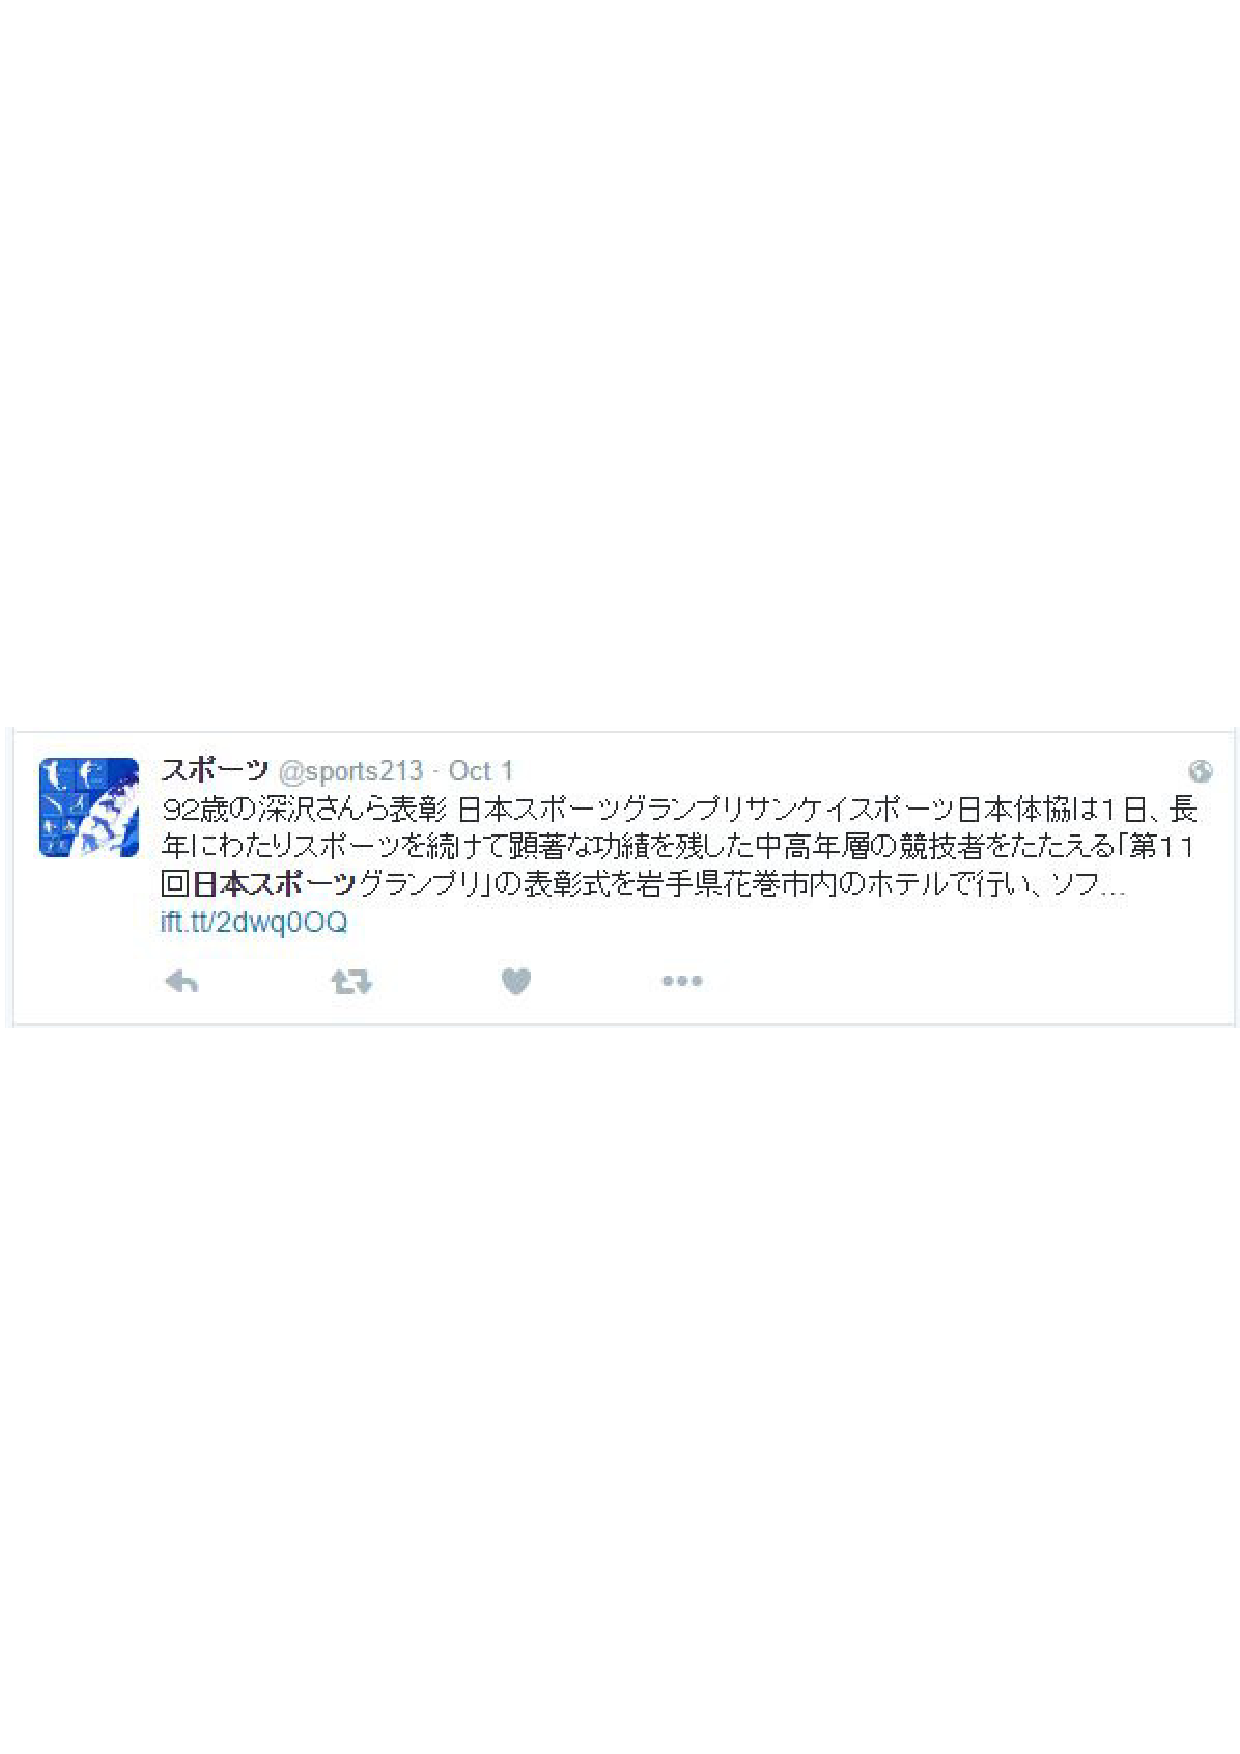
\includegraphics[width=10cm]{tuito.pdf}
\caption{ツイートの例}\label{ace}
\end{figure}

\subsubsection*{ユーザー}
Twitterを利用している者を指す.
 
\subsubsection*{ユーザー名}
半角英数字,アンダーバーから計15文字以内で作るユーザーの名前である.


\subsubsection*{タイムライン}
ユーザー自身のホーム画面のことである.フォローしているユーザーのつぶやきや,自身のつぶやき,リツイートされたツイートなどの情報が羅列されていく.
\begin{figure}[htb]
\centering
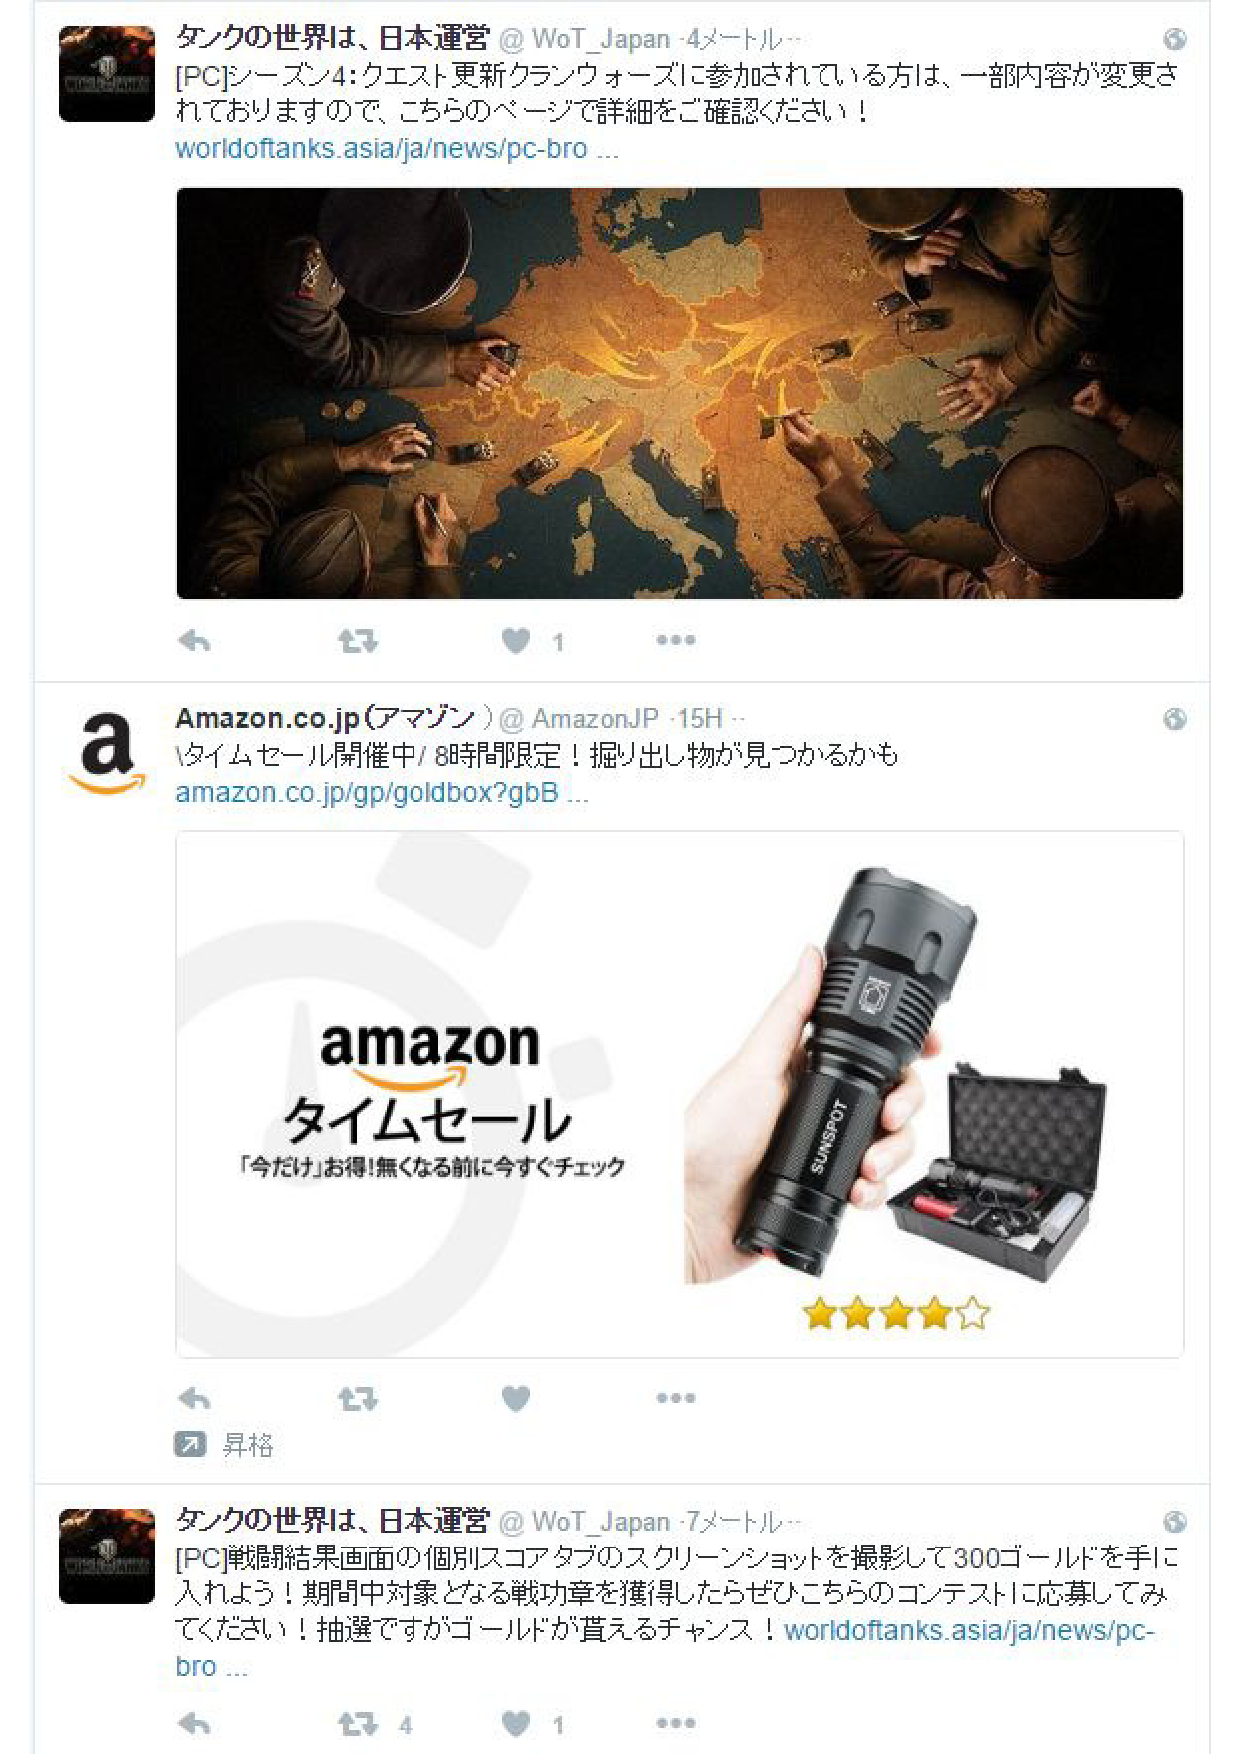
\includegraphics[width=10cm]{taimurain.pdf}
\caption{タイムラインの例}\label{ace}
\end{figure}


\clearpage
\subsubsection*{フォロー}
フォローボタンを押すことによって,ユーザーをフォローして自分のタイムラインにそのユーザーのつぶやきが表示されるようになる.



\subsubsection*{フォロワー}
自分をフォローしているユーザーのことである.フォロワーのタイムラインに自分(フォローされている人)のつぶやきが表示される.


\subsubsection*{リツイート}
他の人のツイートを再びツイートすること.自分のタイムラインに流れてきたツイートをリツイートすると,自分のフォロワーのタイムラインにそのツイートが流れる.逆に自分がフォローしているユーザーがリツイートすると,自分のタイムラインにそのツイートが流れる.


\subsubsection*{リプライ}
特定のユーザー名(@...) から始まるツイートをリプライという.そのユーザー宛のツイートということになる.リプライを送った側と,送られた側の両方をフォローしているユーザーのタイムラインには表示されるが,片方のみをフォローしている第三者のタイムラインには表示されない.


\subsubsection*{お気に入り}
あとで読み返したいツイートをお気に入りに入れてTwitter 上でログ(記録) 化することができる.自分のツイートを含む,全てのツイートに対して有効.発言者がツイートを削除した場合,お気に入りからも削除される.

\subsubsection*{メンション}
特定の「@ユーザー名」を含むツイート.リプライと違って,ツイート内のどこに「@ユーザー名」が入っていてもよい.

\section{Twitterのアカウント登録}
Twitterのアカウント登録方法を記載する.
初めに,Twitterの公式ホームぺージをgoogleで検索し,Twitterのホームページに入る.

\clearpage

\begin{figure}[htb]
\centering
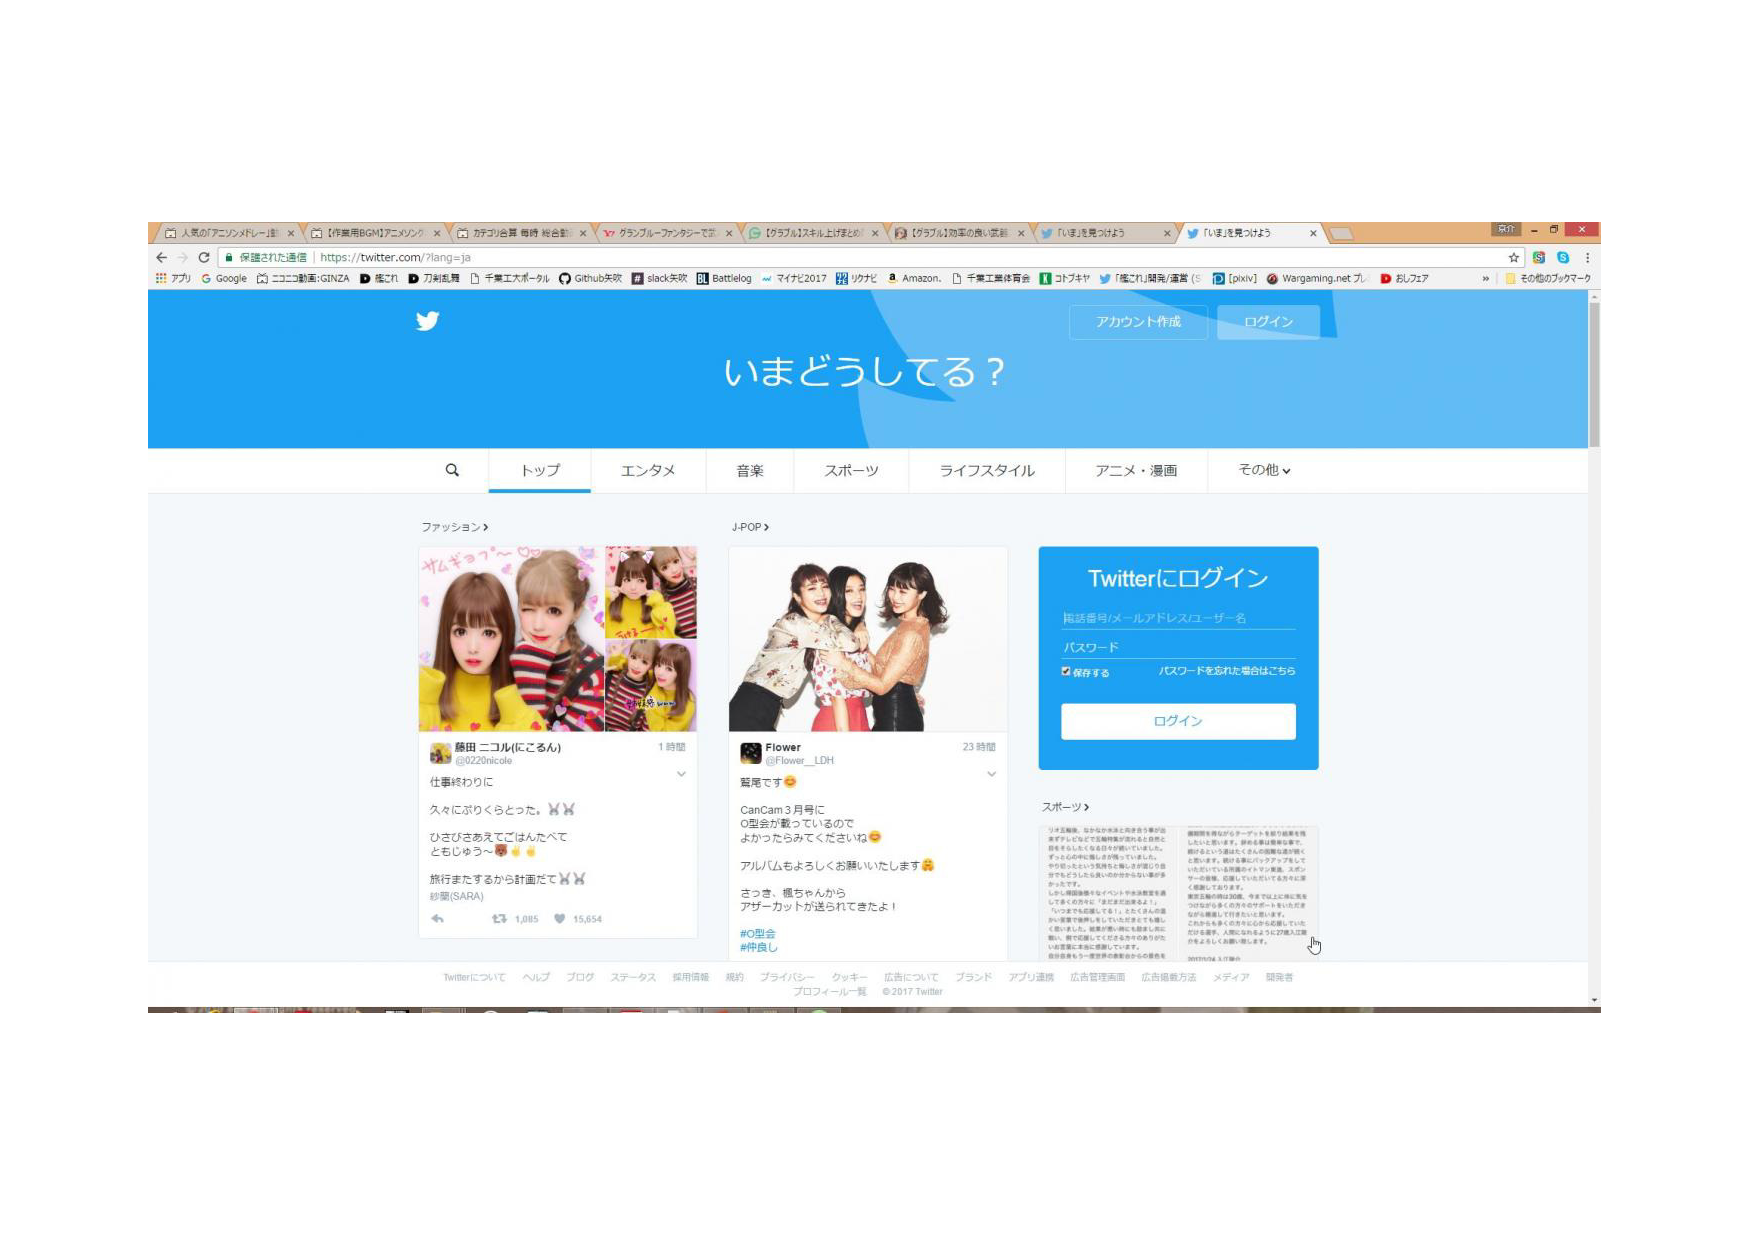
\includegraphics[width=10cm]{twitter10.pdf}
\caption{ツイートの例}\label{ace}
\end{figure}


Twitterのホームページに入ったら,画面右上にある「アカウント作成」をクリックする.
\begin{figure}[htb]
\centering
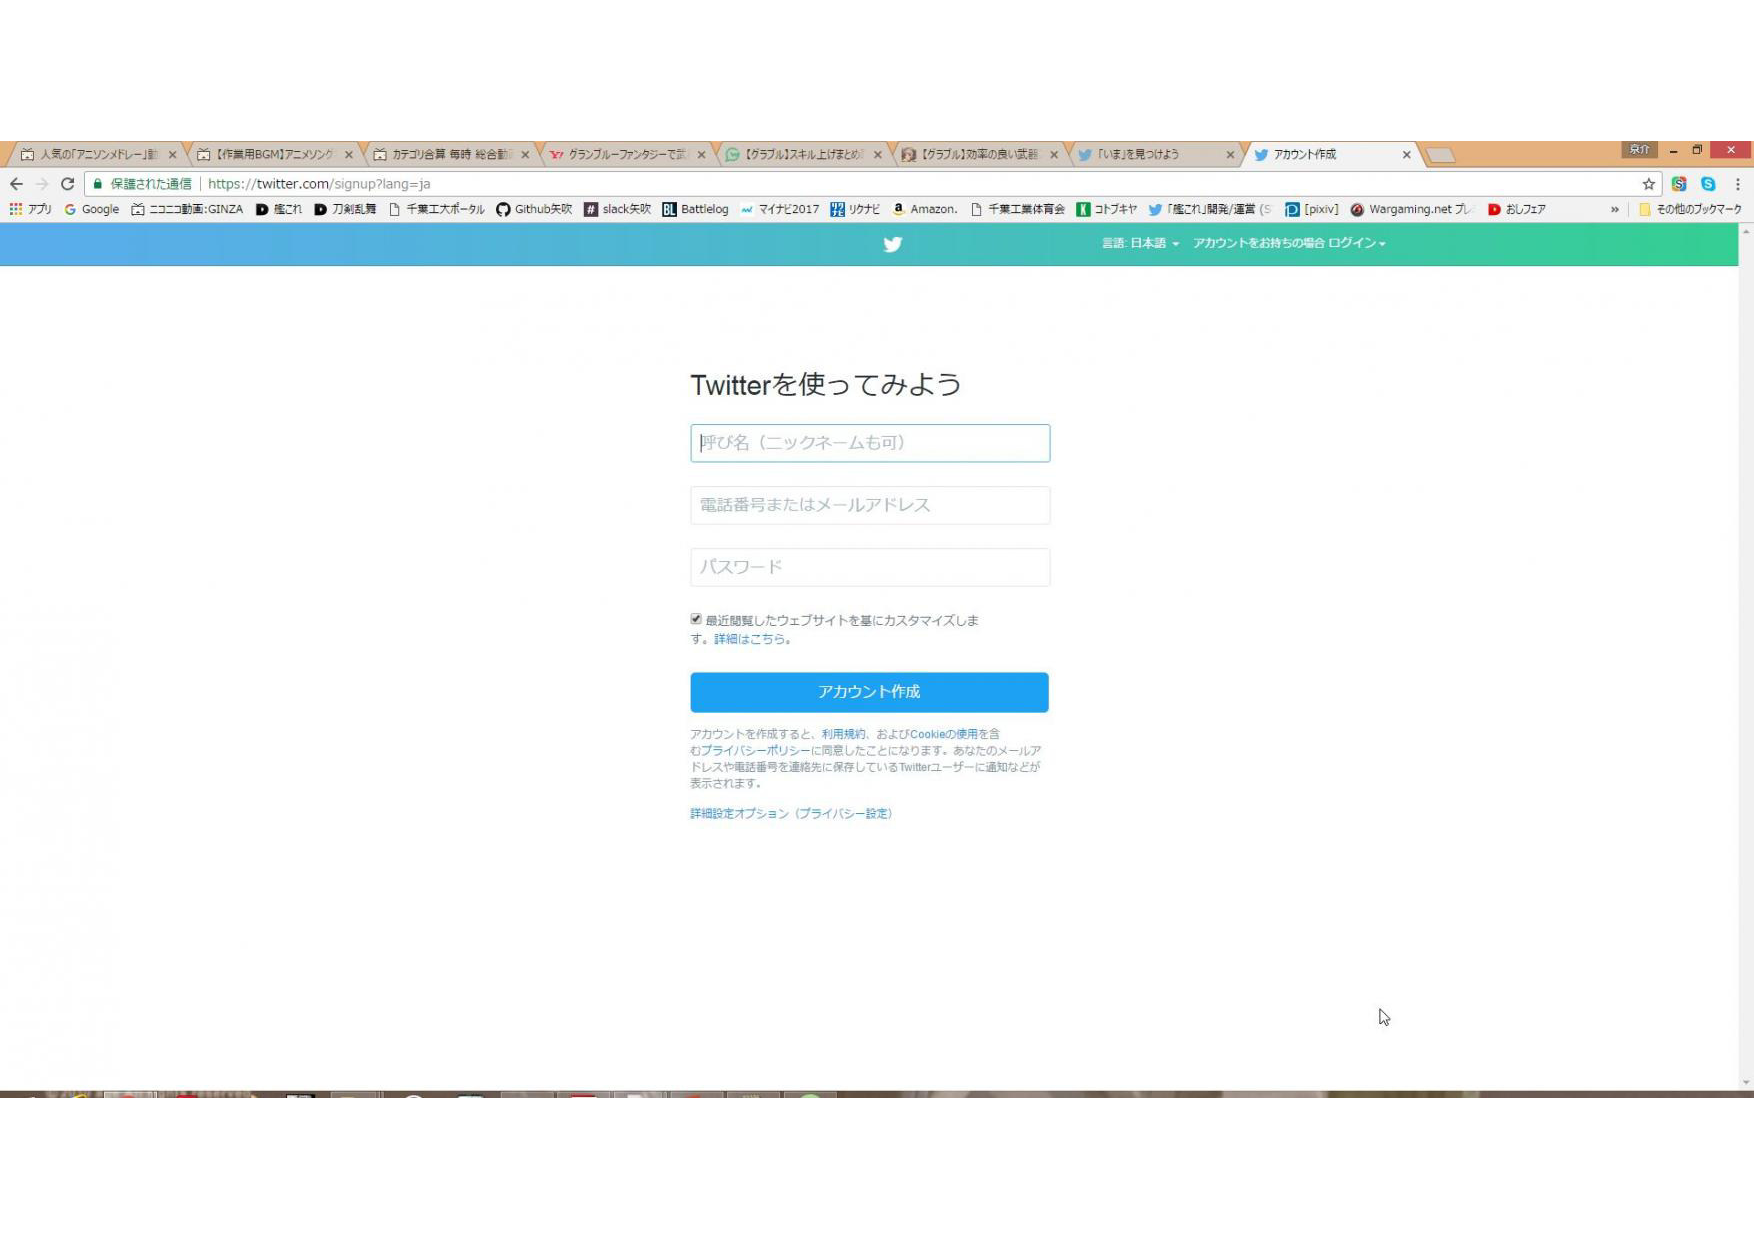
\includegraphics[width=10cm]{twitter15.pdf}
\caption{ツイートの例}\label{ace}
\end{figure}

\clearpage

ここではTwitterを使う際に必要な「ニックネーム」,「電話番号もしくはメールアドレス」,「パスワード」を記載する.その後「アカウント作成」ボタンをクリックする.

\begin{figure}[htb]
\centering
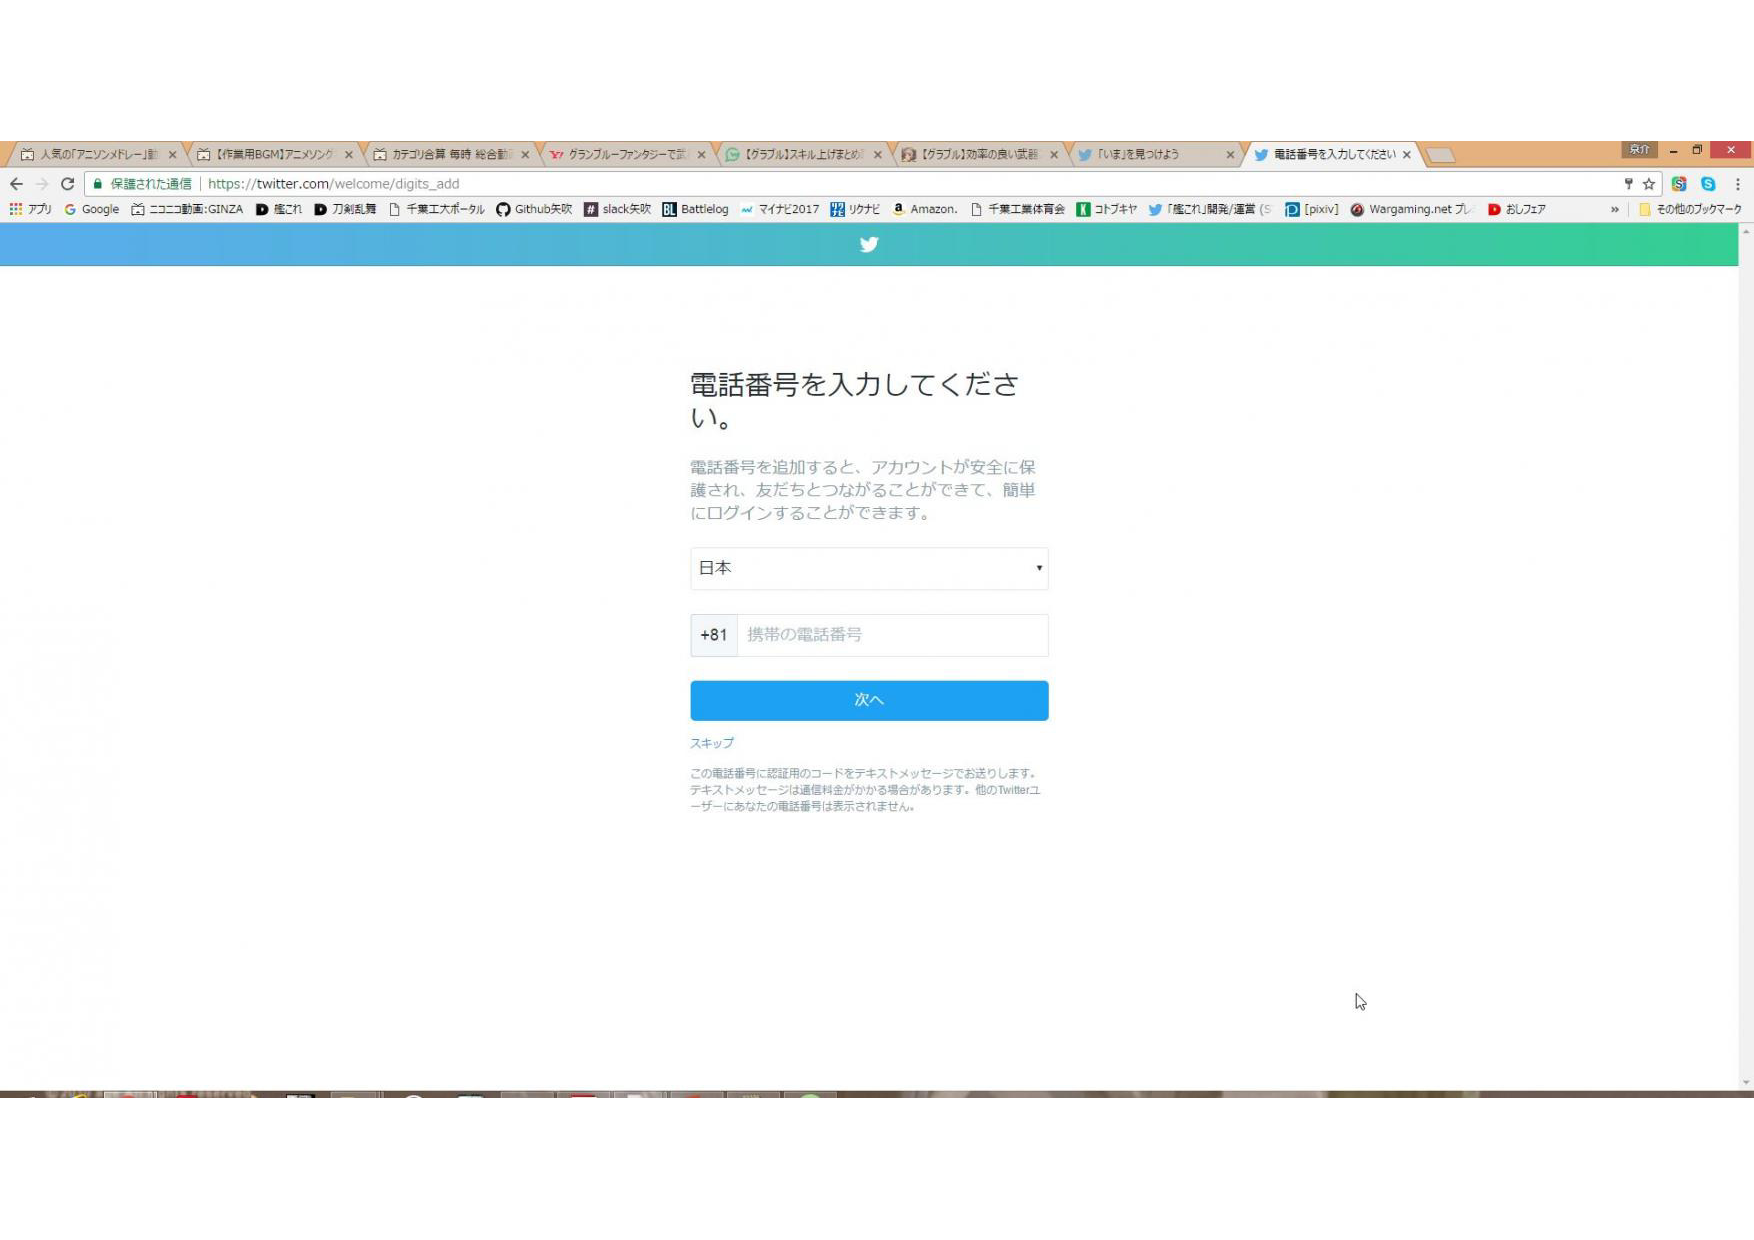
\includegraphics[width=10cm]{twitter20.pdf}
\caption{ツイートの例}\label{ace}
\end{figure}


ここでは電話番号の入力を要求されるが,しなくてもアカウントの登録は可能である.電話番号を入力するのであれば,電話番号の記載を.電話番号を入力しないのであれば「次へ」ボタンの左下にある「スキップ」をクリックする.

\begin{figure}[htb]
\centering
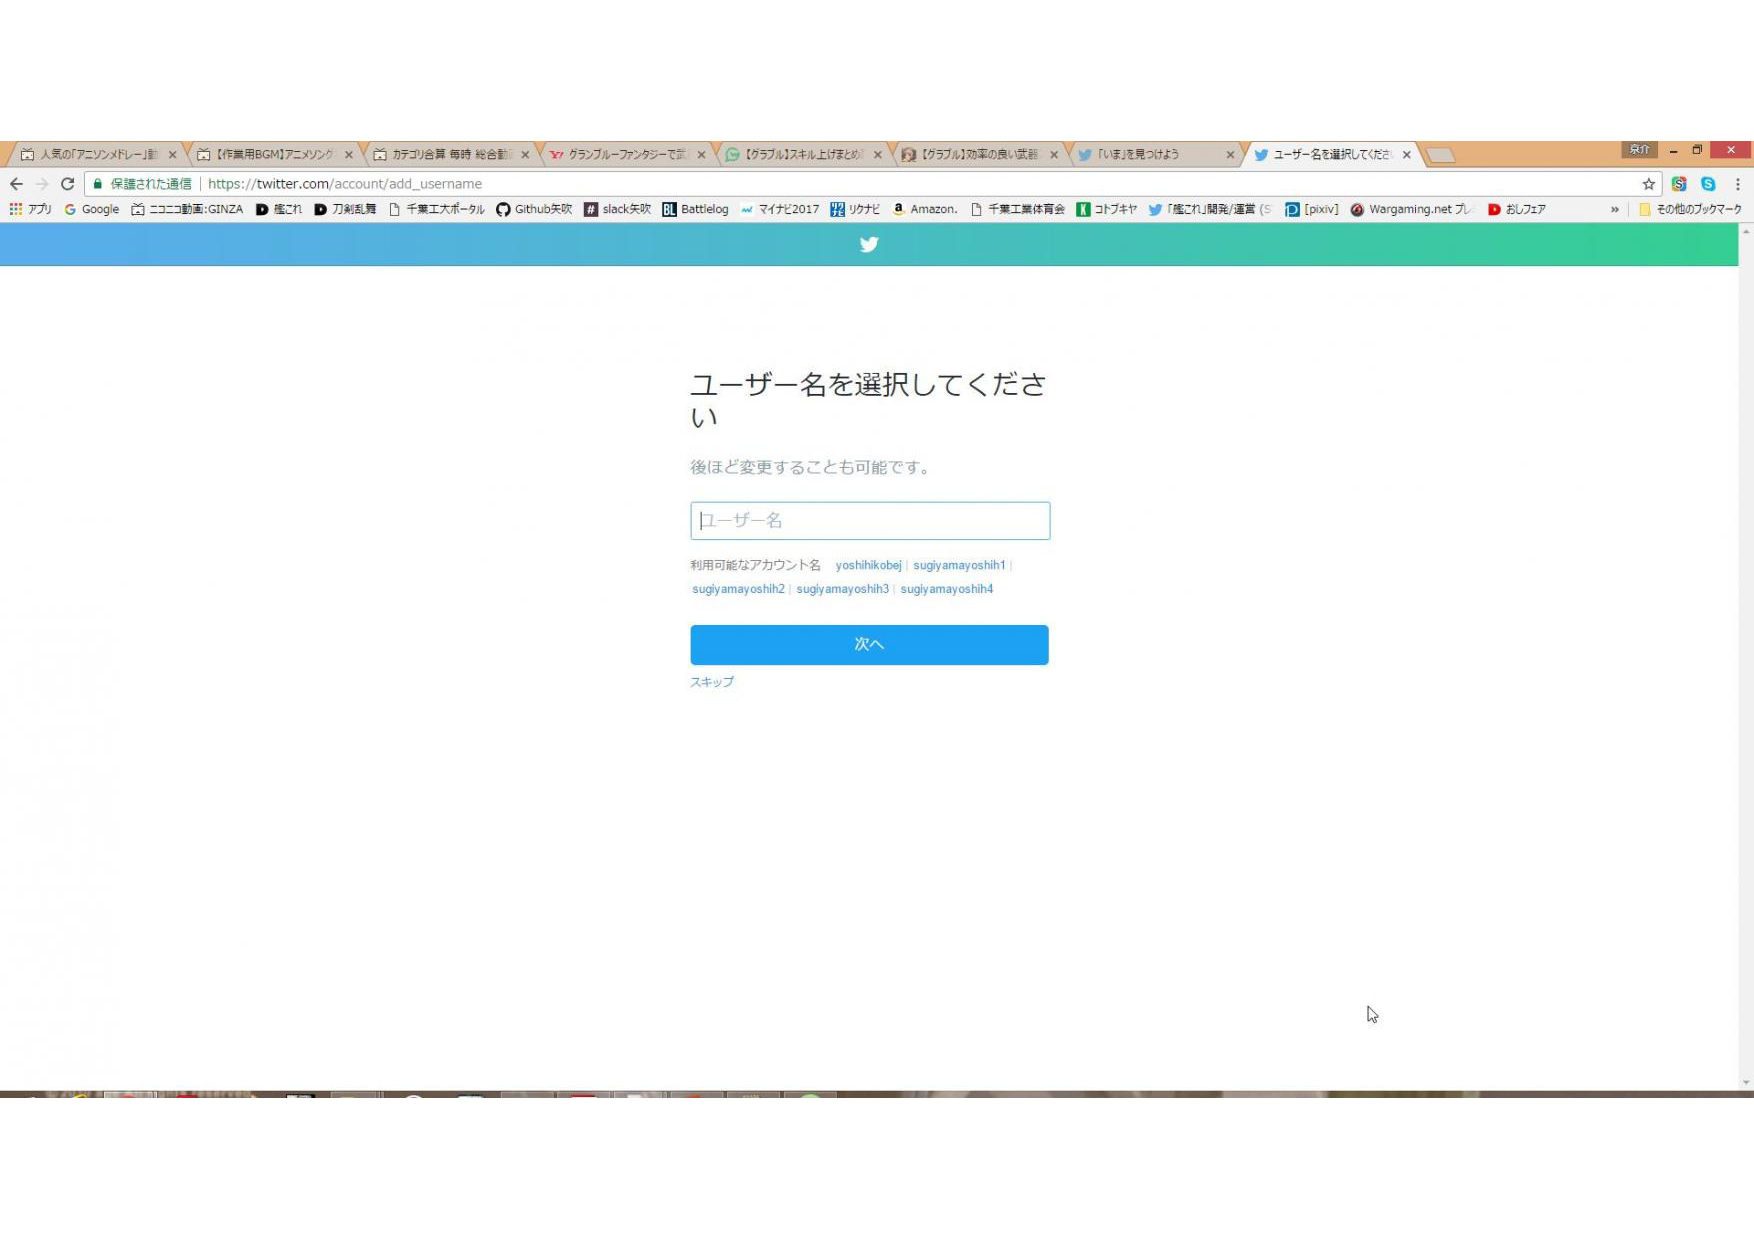
\includegraphics[width=10cm]{twitter25.pdf}
\caption{ツイートの例}\label{ace}
\end{figure}


ここでは,ユーザー名を記入する.もしくは利用可能なアカウント名をクリックして選ぶ.ユーザー名は登録後に変更が可能なため,その時の好きなユーザー名を記入することが出来る.

また記入を行った際に,他のユーザーに使われていると記入ボックスの右隣りに「このユーザー名は既に使用されています。」と表示される.

\begin{figure}[htb]
\centering
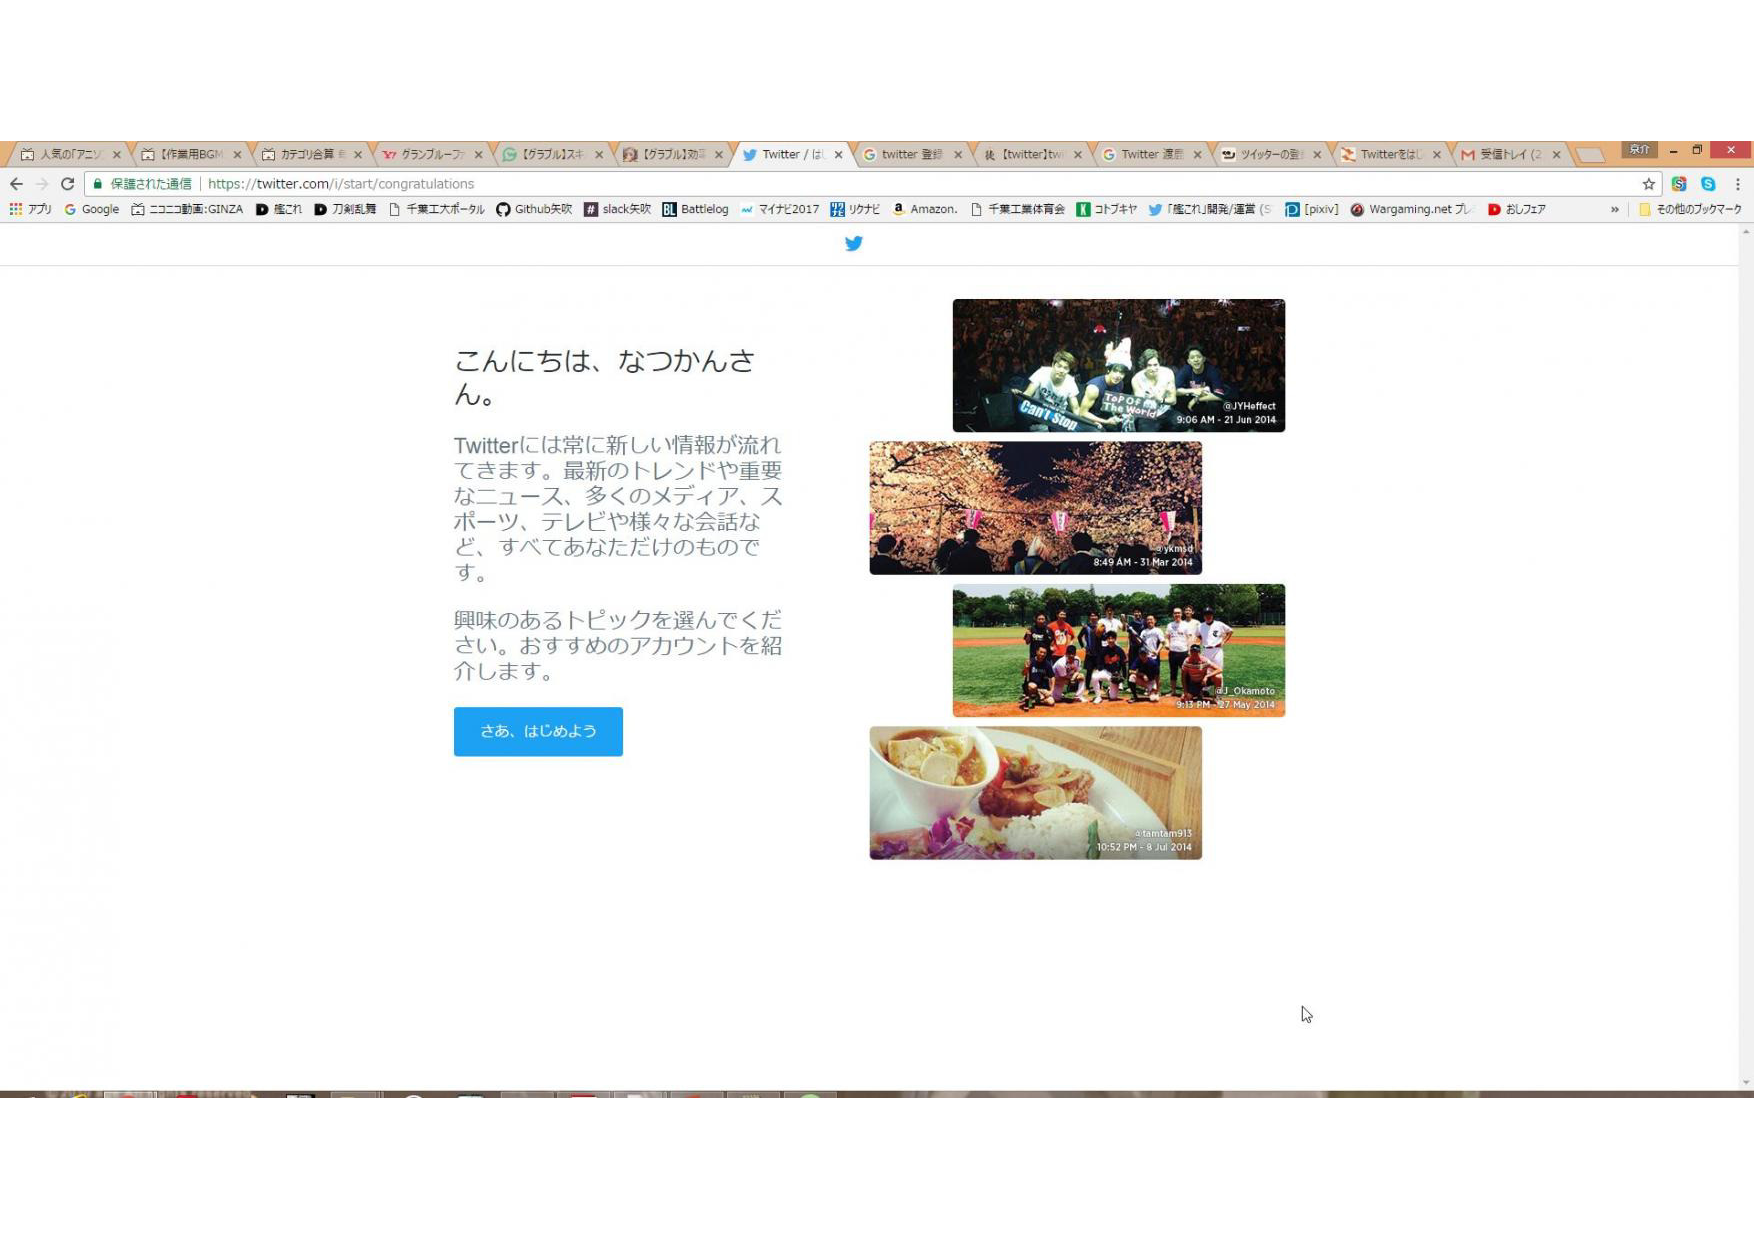
\includegraphics[width=10cm]{twitter30.pdf}
\caption{ツイートの例}\label{ace}
\end{figure}


ユーザー名を決めることができたら,アカウント作成は終了である.







\section{ツイートの収取}
本研究で使用したツイートの収集方法を記載する.

初めに,Twitterのキーワード検索で検索を行う.今回使うキーワードは本章の「5.6ニコニコ動画ランキングAPIの導入」で取得した動画のタイトルを使用する.

次に,キーワード検索の結果が出たら,サイト上部にあるタブの{すべてのツイート」を選択する.次に,自分が取りたい日にちのツイートまでスクロールを行う.

\clearpage

\begin{figure}[htb]
\centering
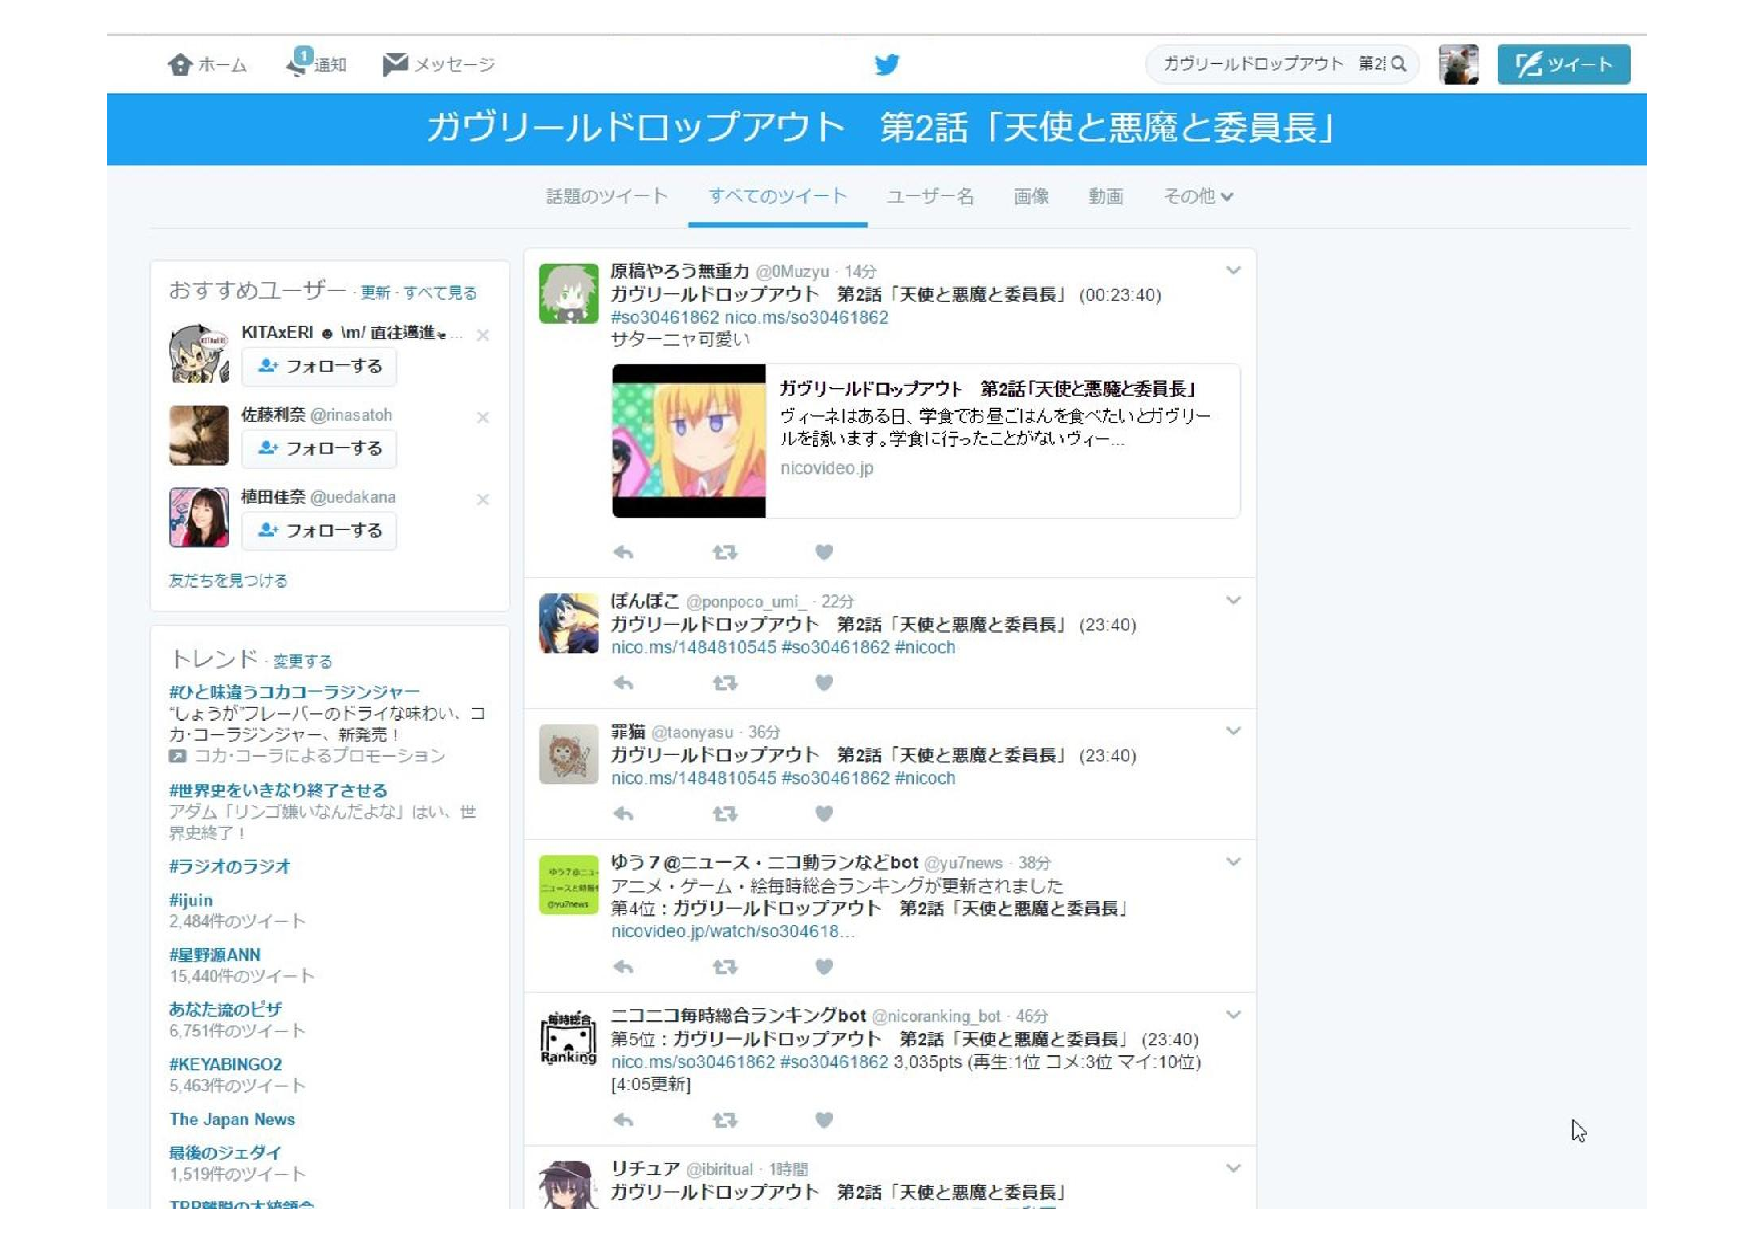
\includegraphics[width=10cm]{tuiito10.pdf}
\caption{ツイートの検索結果}\label{ace}
\end{figure}



自分が取りたい日にちへスクロールを終えたら,サイト上で右クリックを行い「名前を付けて保存」を選択する.名前は英数字にし,保存先は作業ディレクトリの中にする.

次に,保存したファイルの中にrocal.rbを作成し,この中にコードを書いていく.

コードは,
	\begin{verbatim}
# -*- coding: utf-8 -*-
require 'nokogiri'

file = File.open("gauriru.html")
doc = Nokogiri::HTML(file)
doc.xpath("//li[@data-item-type='tweet']").each { |tweet|

	# Tweet時間
	puts Time.at(tweet.xpath(".//a[@class='tweet-timestamp js-permalink js-nav js-tooltip']/span").first['data-time'].to_i)
	# Tweet本文
	puts tweet.xpath(".//p[@class='TweetTextSize  js-tweet-text tweet-text']").text
}

	\end{verbatim}
である.
今回は,「gauriru.html」というデータファイルを使用する.他のデータファイルを選択したい場合は,file = File.open("gauriru.html")の引用符の間の名前を変更する.

次に,コマンドプロプトで「rocal.rb」が保存されているファイルまで移動したら,

ruby rocal.rb

とコマンドプロプトへ書き込み起動するとデータが読める.

取得したデータはこのように表示される.
	\begin{verbatim}
2017-01-24 05:46:49 +0900
ガヴリールドロップアウト 第2話「天使と悪魔と委員長」 (23:40) http://nico.ms/1484810545  #so30461862 #nicoch

以降のデータは省略する.
	\end{verbatim}
以上が,本研究においてTwitterからのツイートのデータの取集方法である.

\chapter{クローラーについて}


\section{本章の構成}

本章では本研究で使用するクローラーの作成方法ついて記す.


\section{クローラーとは}
クローラー(Crawler)は,Googleなどのロボット型検索エンジンがWeb上のファイルを収集するためのプラグラムのことである.「ボット」,「スパイダー」「ロボット」とも呼ばれる.

\section{パッケージの導入}
本研究でクローラーを使用するためのパッケージとして,Chocolatey,atom,vagrantの導入方法を記載する.

\subsubsection*{Chocolateyとは}
ChocolateyはWindows上で動作するソフトウェアをコマンドラインからインストール/アンインストール/アップデート/検索することができるパッケージマネージャーである.
Chocolateyのリポジトリに登録されているパッケージのインストールと依存するパッケージのインストールを行う.(例 Scalaをインストールした場合,jreも一緒にインストールを行ってくれるものである.)

リポジトリに登録されているパッケージを抜粋する.

ブラウザ (Google Chrome, Firefox)

バージョン管理ツール (Git, Subersion, Mercurial)およびバージョン管理のGUIクライアント

IDE (Intellij IDEA, Eclipse)

エディタ (Atom, Sublime)

各プログラミング言語の実行環境(JavaScript(Node.js), Ruby, Python, Java, Scala, Groovy ...etc)

仮想(VirtualBox, Vagrant)

などがあった.

コマンドラインから一発でパッケージをインストールできるため、研究で開発環境を構築する時に使用する.
また、インストールするパッケージを書いたxml(packages.config)からインストールすることもできるため、プロジェクト内の開発環境を統一することにも使る.


\subsubsection*{Atomとは}
Atomとは,GitHubの創業者Chris Wanstrath氏が「Web技術を用いて、Emacsのように自由にカスタマイズできる新世代のエディターを開発する」という思いから始まったオープンソースのエディターである.\cite{atom}

\subsubsection*{vagrantとは}


\subsubsection*{vagrantのコマンド}
\begin{table}[htb]
	\begin{center}
		 \caption{仮想マシンの操作}
 			\begin{tabular}{|l|c|r||r|} \hline
				コマンド & 解説  \\ \hline \hline
				vagrant up & 仮想マシンの起動。vagrantfileのあるディレクトリ内で実行  \\ \hline
				vagrant halt & 仮想マシンの終了(シャットダウン)  \\ \hline
				vagrant suspend & 仮想マシンの一時停止  \\ \hline
				vagrant resume & 仮想マシンの一時停止から復帰  \\ \hline
				vagrant reload & ≒ halt → up \\ \hline
				vagrant provision & 仮想マシンは起動したままプロビジョニングのみ再度実行  \\ \hline
				vagrant destroy & 仮想マシンの削除(boxは消えない)  \\ \hline
				vagrant status & 仮想マシンのステータスを表示  \\ \hline
				vagrant ssh & 仮想マシンにログイン  \\ \hline
				vagrant ssh-config & sshログイン時の設定確認。IdentityFileは秘密鍵の場所  \\ \hline
				vagrant reload --provision & 設定ファイル(site.yml)を変更したらこのコマンドで反映  \\ \hline
				vagrant version & バージョン確認+細心バージョンの表示 (vagrant -vはバージョン確認のみ)  \\ \hline
				vagrant -h & ヘルプ  \\ \hline
			\end{tabular}
	 \end{center}
\end{table}

\begin{table}[htb]
	\begin{center}
		 \caption{boxの一覧、追加、アップデート、削除}
 			\begin{tabular}{|l|c|r||r|} \hline
				コマンド & 解説  \\ \hline \hline
				vagrant box list box& boxの一覧を表示  \\ \hline
				vagrant box add **/** & boxの追加。Vagrant Cloud、\\ & ローカルのbox、URLから取得  \\ \hline
				vagrant box add & 付けたい名前 box名.box  \\ \hline
				vagrant box update --box **/** & vagrantのアップデート  \\ \hline
				vagrant init BOX NAME & 初期化(Vagrantfileの作成)  \\ \hline
				vagrant box remove **/** & boxの削除  \\ \hline
				vagrant box remove **/** --box-version 0.0.1 & boxの削除(バージョン指定)  \\ \hline
				vagrant package box名 & 現在の仮想マシンをboxに。box名省略なら元のbox名  \\ \hline
			\end{tabular}
	 \end{center}
\end{table}

\begin{table}[htb]
	\begin{center}
		 \caption{boxの一覧、追加、アップデート、削除}
 			\begin{tabular}{|l|c|r||r|} \hline
				コマンド & 解説  \\ \hline \hline
				vagrant snapshot push & 単一スナップショット作成  \\ \hline
				vagrant snapshot pop & 単一スナップショット復元  \\ \hline
				vagrant snapshot save <スナップショット名> & 名前付きスナップショット作成  \\ \hline
				vagrant snapshot restore <スナップショット名> & 名前付きスナップショット復元  \\ \hline
				vagrant snapshot list & 名前付きスナップショットの一覧を表示  \\ \hline
			\end{tabular}
	 \end{center}
\end{table}

\begin{table}[htb]
	\begin{center}
		 \caption{Vagrant Cloud}
 			\begin{tabular}{|l|c|r||r|} \hline
				コマンド & 解説  \\ \hline \hline
				vaglant login & ログイン \\ \hline
				vagrant share & ローカル環境を公開。表示されるURLで外部からアクセス可能に。 \\
				                              & Ctrl + C で終了 \\ \hline
				vagrant connect xxxxx & SSHなどでの接続も可能。セキュリティ的リスクあるが便利な場面も \\
				                                 & "hashicorp/precise32"のような名前のboxが作られる。終了しても \\
				                                 & 残るので、要らなくなったらこのboxは手動で削除する \\ \hline
			\end{tabular}
	 \end{center}
\end{table}

\clearpage

\subsubsection*{Chocolatey,Atom,vagrantの導入}
初めに,管理者用のコマンドプロプトで以下のコードを実行する.
	\begin{verbatim}
cinst -y atom chrome curl git github r.project rsync sourcetree vagrant 
virtualbox wget
	\end{verbatim}
Chocolatey,Atom,vagrantが入っているか確かめるため,管理者用ぼコマンドプロプトに choco list -lo を書き込む.

\section{vagrantを使用した仮想マシンの構築}
この作業はChocolateyのパッケージが入っている必要がある.

初めに,管理者用ではないコマンドプロプトを起動する.次に,仮想マシンを用意するためのコードを管理者用ではないコマンドプロプトへ書き込んでいく.
コードは,
	\begin{verbatim}
c:
cd \
mkdir vagrant
cd vagrant
git clone https://github.com/yabukilab/machine.git
	\end{verbatim}
である.

次に,先ほど作った仮想マシンを起動する.

コードは,
	\begin{verbatim}
c:
cd \vagrant\machine
vagrant up
	\end{verbatim}
である.

次に,仮想マシンにゲストとして絶族する.ホストにいる場合,\begin{verbatim}C:\vagrant\machine \end{verbatim}へ移動する.そこで vagrant ssh を行う.ゲストとして接続すると,vagrant@vagrant-ubuntu-trusty-64 と表示される.

\section{クローラーの導入}
vagrant上でクローラーを運用する手順を解説する.

初めに,今回使用するクローラーのプログラムはシェルで書く.説明のため,ファイル名は「while.sh」とする.

「while.se」の内容は以下のとおりである.

\begin{figure}[htb]
\centering
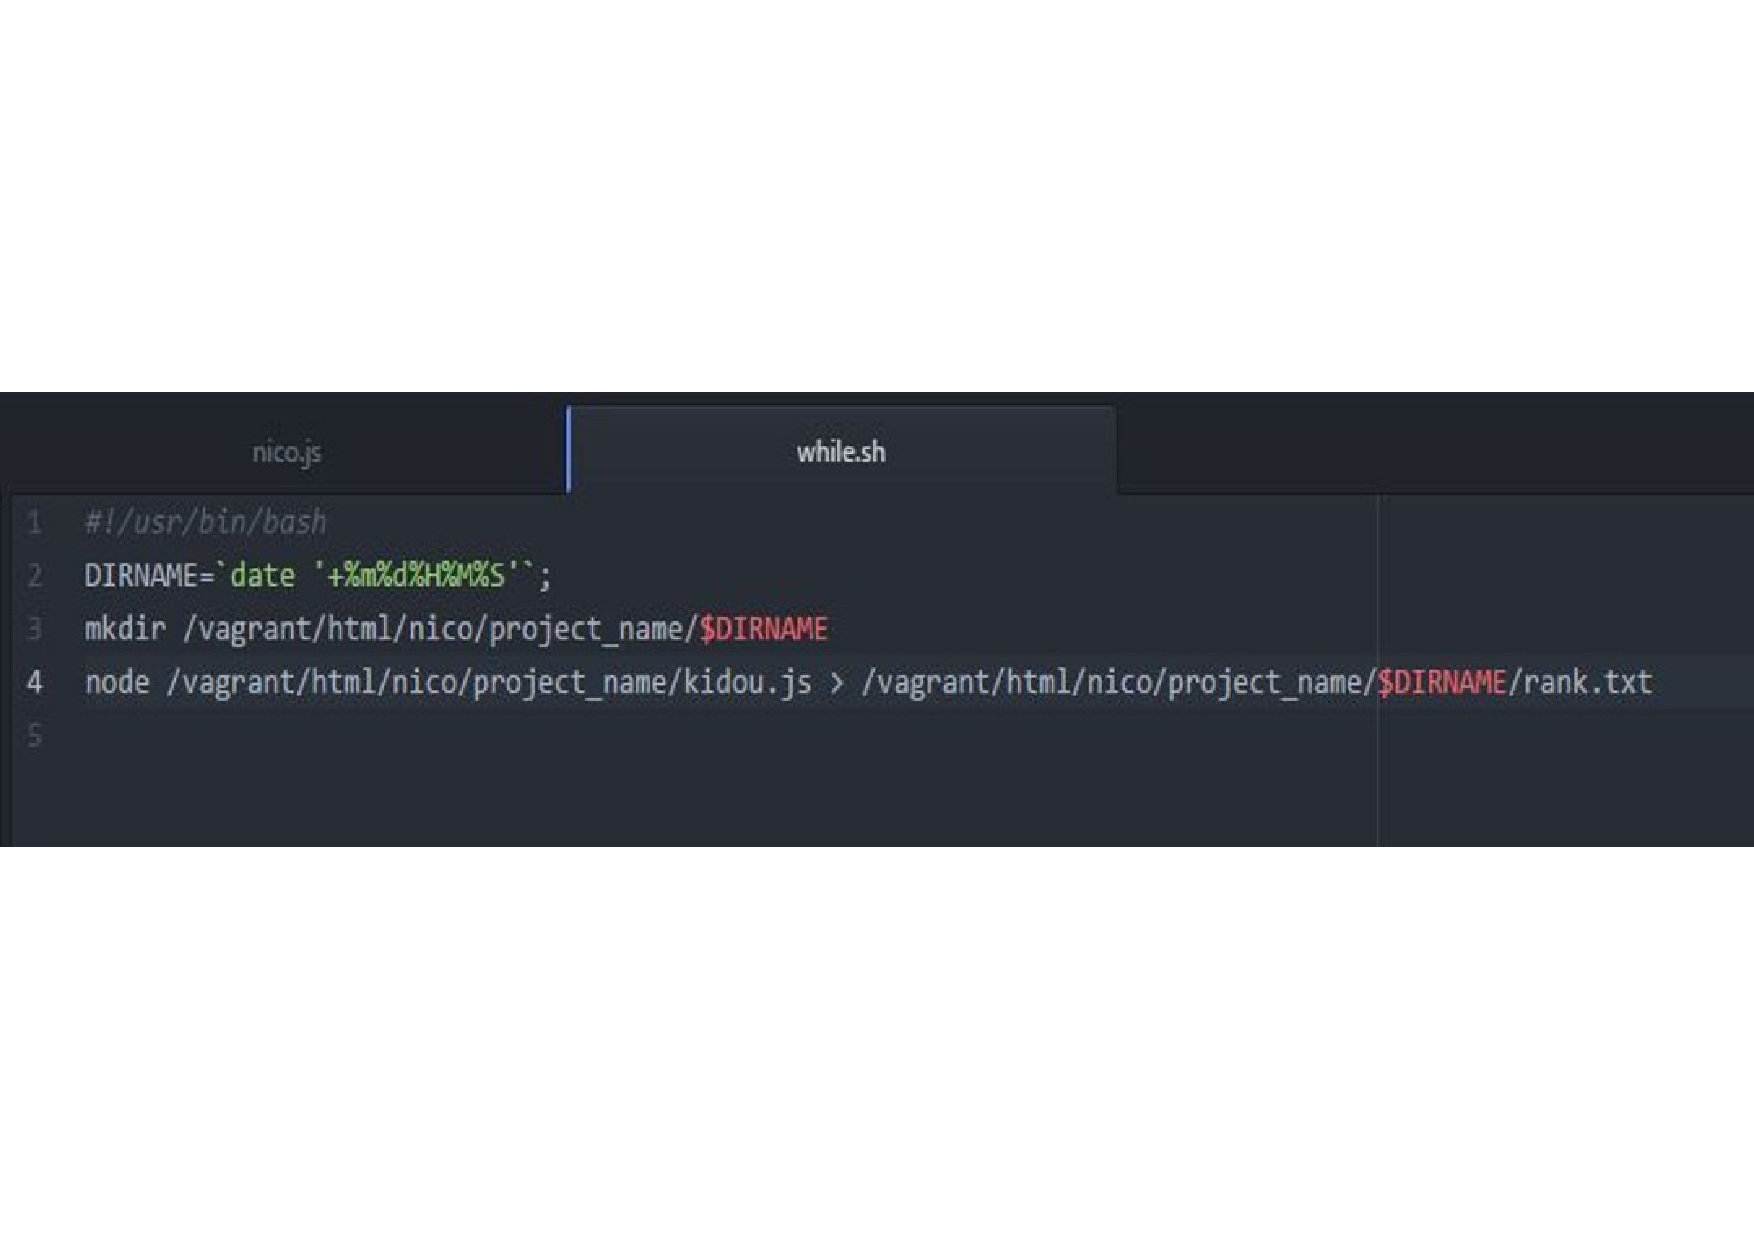
\includegraphics[width=16cm]{while.pdf}
\caption{ツイートの例}\label{ace}
\end{figure}


内容の中にある「kidou.js」は「5,6 ニコニコ動画ランキングAPIのモジュールの呼び出し」に記載されている.

毎日,毎時間毎にデータを収集するため,同じフォルダで保存し続けるのを避けるため,Linuxコマンドのdata,cd,mkdirを組み合わせてプログラムが動き出した現在時刻をフォルダ名に設定するようにしてある.以下に今回使用したコマンドの解説を記す.

\begin{table}[htb]
	\begin{center}
		 \caption{日付,時刻を表示,設定する}
 			\begin{tabular}{|l|c|r||r|} \hline
      文字 & 解説  \\ \hline \hline
\%H & 時 (00~23) \\ \hline
\%I & 時 (01~12) \\ \hline
\%k & 時 ( 0~23) \\ \hline
\%l & 時 ( 1~12) \\ \hline
\%M & 分 (00~59) \\ \hline
\%p & AM あるいは PM のロケール(国や地域に合わせた文字列) \\ \hline
\%r & 12時間形式の時刻 (HH:mm:ss [AP]M) \\ \hline
\%s & 1970-01-01 00:00:00 UTC からの秒数 \\ \hline
\%S & 秒 (00~61) \\ \hline
\%T & 24時間形式の時刻 (HH:mm:ss) \\ \hline
\%a & ロケールによる省略形の曜日の名前 (Sun~Sat) \\ \hline
\%A & ロケールによる完全に表記した曜日の名前(Sunday~Saturday) \\ \hline
\%b & ロケールによる省略形の月の名前 (Jan~Dec) \\ \hline
\%B & ロケールによる完全に表記した月の名前(January~December) \\ \hline
\%c & ロケールによる日付と時刻 (Sat Nov 04 12:02:33 EST 1989) \\ \hline
\%d & 日(月内通算日数) (01~31) \\ \hline
\%D & 日付 (MM/DD/YY) \\ \hline
\%j & 年内通算日数 (001~366) \\ \hline
\%m & 月 (01~12) \\ \hline
\%w & 週のうちの曜日(0~6)で0が日曜日に対応 \\ \hline
\%x & ロケールによる日付の表現 (MM/DD/YY) \\ \hline
\%y & 西暦の下2けた (00~99) \\ \hline
\%Y & 年 (1970~) \\ \hline
			\end{tabular}
	 \end{center}
\end{table}


\begin{table}[htb]
	\begin{center}
		 \caption{ディレクトリの移動する}
 			\begin{tabular}{|l|c|r||r|} \hline
      文字 & 解説  \\ \hline
   / & ルート・ディレクトリ \\
    . & 現在のディレクトリ \\
   … & 親ディレクトリ \\
  \~/ & ホーム・ディレクトリ \\ \hline
			\end{tabular}
	 \end{center}
\end{table}


\begin{table}[htb]
	\begin{center}
		 \caption{ディレクトリを作成する}
 			\begin{tabular}{|l|c|r||r|} \hline
      文字 & 解説  \\ \hline \hline
   -m & ディレクトリのモードを設定する \\ \hline
    -p & 指定したディレクトリをサブディレクトリごと作成する. \\ \hline
   -v & ディレクトリを作成する毎にメッセージを出力する \\ \hline
   --help & mkdirコマンドの使用法を表示する \\ \hline
--version	& バージョン情報を標準出力に表示する \\ \hline
directory & 作成するディレクトリ名を指定する \\ \hline
			\end{tabular}
	 \end{center}
\end{table}



	\begin{verbatim}
vagrant@vagrant-ubuntu-trusty-64:/$ crontab -u vagrant -e
1. /bin/ed
2. /bin/nano <---- easiest
3. /usr/bin/vim.basic
4. /usr/bin/vim.tiny


Choose 1-4 [2]:
	\end{verbatim}

\begin{figure}[htb]
\centering
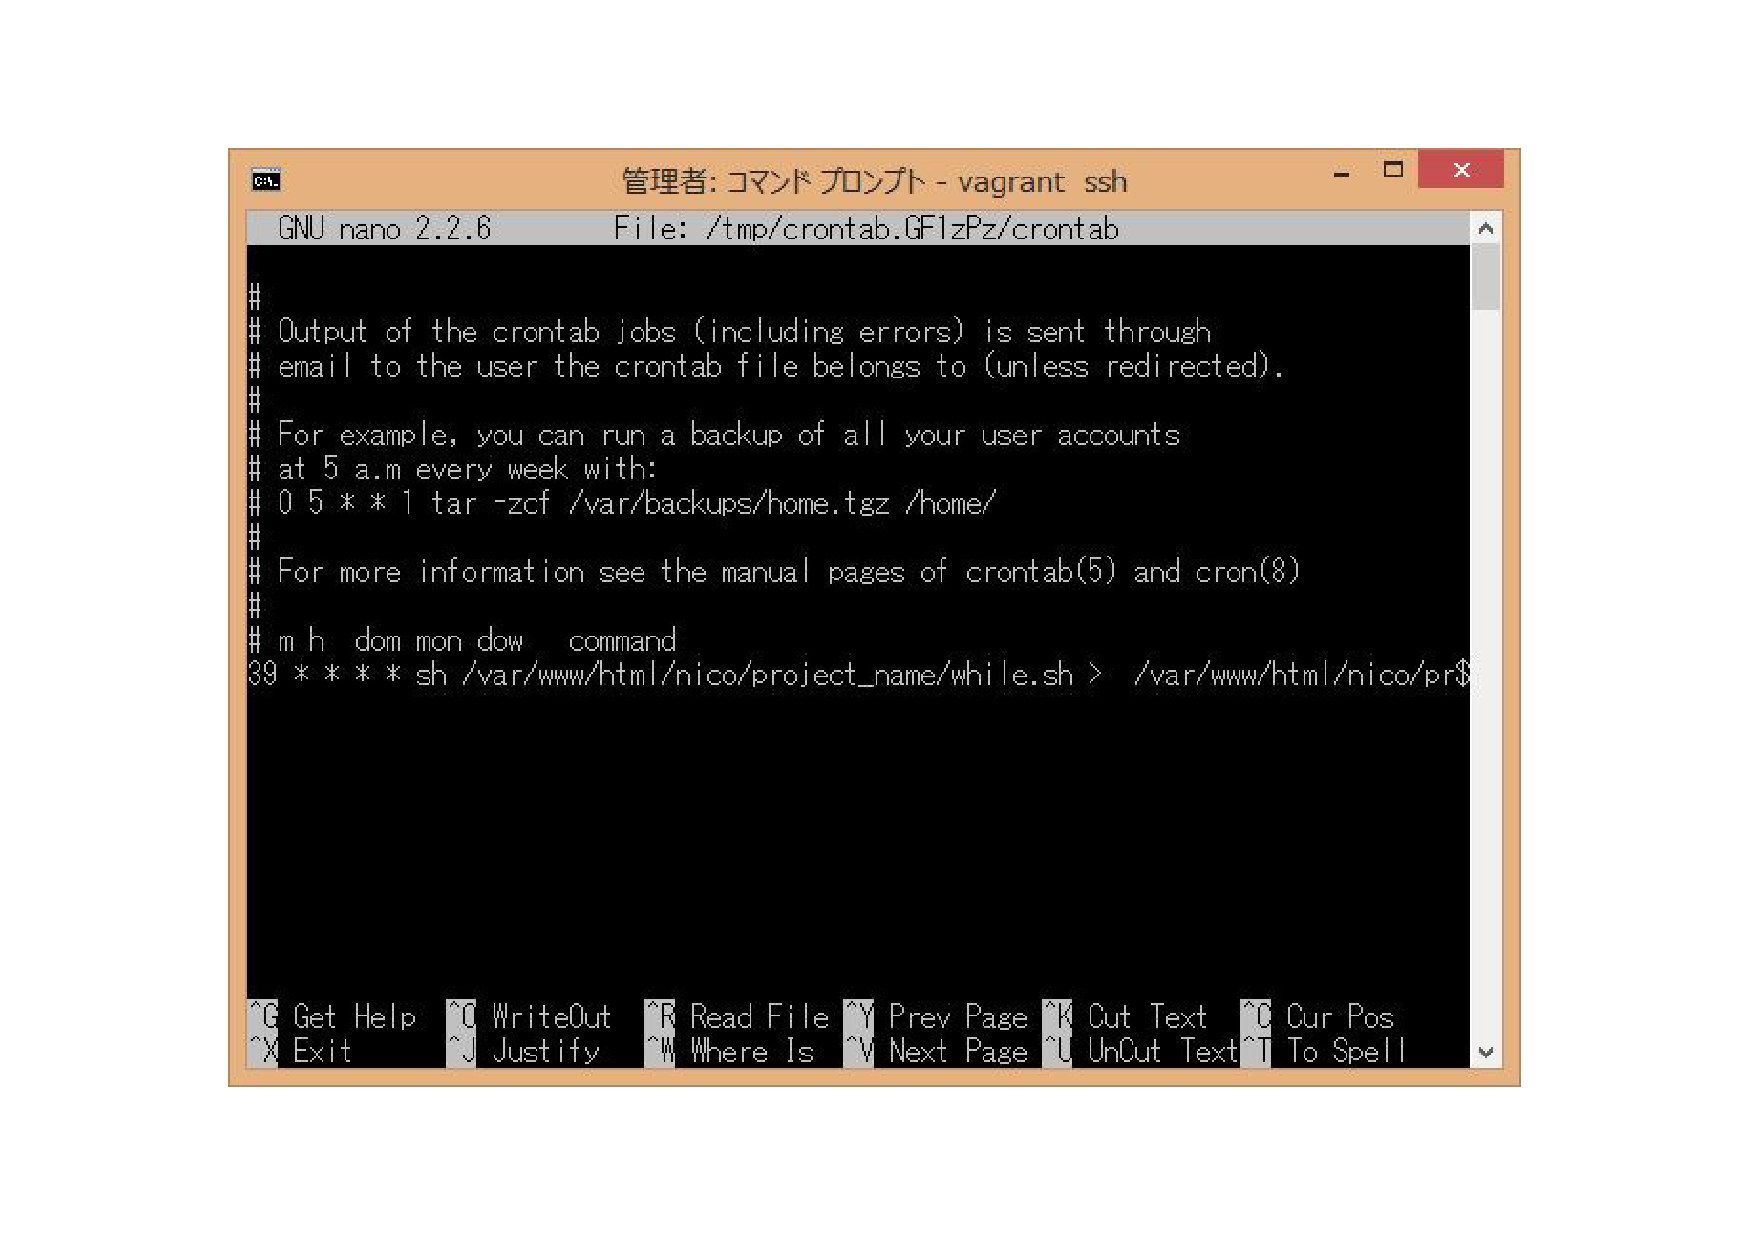
\includegraphics[width=14cm]{crontab10.pdf}
\caption{クローラーの導入}\label{ace}
\end{figure}

\clearpage

vagrant上にあるシェルを毎日,網時間毎に自動で動かすために,端末からcrontabを利用して時間が来たらシェルを呼び出し,プログラムをスタートするように設定する.
端末を起動し,crontab -u ユーザー名 -e と入力をし,Enterを押す.
表示された3つの選択肢の中から好きなエディターを選ぶことができる.今回は2を選択する.
2を入力しEnterを押すと下記の画面が表示される



エディターでプログラムを行う時刻とプログラムを指定する.文法は以下のとおりである.

分 時 日 月 曜日 コマンド

\begin{table}[htb]
	\begin{center}
		 \caption{ディレクトリを作成する}
		 \begin{tabular}{|l|c|r||r|} \hline
      文法 & 解説   \\ \hline \hline
分 & 分を「0~59」で指定する。ワイルドカード(*)を \\
	& 記述すると毎分となる。 \\ \hline
時 & 時間を「0~23」で指定する。ワイルドカード(*)を\\
	& 紀述すると毎時となる。 \\ \hline
日 & 日を「1~31」で指定する。ワイルドカード(*)を\\
	& 記述すると毎日となる。 \\ \hline
月 & 月を「1~12」もしくは「jan~dec」で指定する。\\
	& ワイルドカード(*)を記述すると毎月となる。 \\ \hline
曜日 & 曜日を「0~7」(0,7は日曜日)もしくは「sun~sat」\\
	 &で指定する。ワイルドカード(*)を記述すると毎日となる。 \\ \hline
コマンド & 実行したいコマンドやシェルを記述します。 \\ \hline
			\end{tabular}
	 \end{center}
\end{table}

今回のクローラーの稼働設定を例としてあげると,
\begin{verbatim}
39 * * * * sh /var/www/html/nico/project_name/while.sh >
  /var/www/html/nico/project_name/cron_error2.txt

毎時間,39分に/var/www/html/nico/project_name/の中にあるwhile..shを実行し,/var/www/html/nico/project_name/の中にクローラーがエラーした場合のエラーコードをcron_error2.txtに保存するという命令になる.
\end{verbatim}

\chapter{手法}

\section{本章の構成}
本章では,研究方法と実際に行った研究手順について記載する.

\section{研究方法}

以下の手法で研究を行う.

\begin{enumerate}

\item ニコニコ動画のカテゴリ合算毎時総合ランキングの1位から100位までの投稿動画の再生数を1時間毎に抜き出す.
\item 時間毎に増加していく再生数の累積のグラフを作成する.このグラフを①とする.
\item 再生数の増加を1時間毎に区切ったグラフを作成する.このグラフを②とする.
\item Twiiterでニコニコ動画のカテゴリ合算毎時総合ランキングの1位から100位までの動画の名前でツイートの検索し,1時間毎にツイート数を抜き出す.
\item 時間毎に増加していくツイート数の累積させたグラフを作成する.このグラフを③とする.
\item ツイート数の増加を1時間毎に区切ったグラフを作成する.このグラフを④とする.
\item ①と③,②と④の2通りの比較を行い,カテゴリ合算毎時総合ランキングとTwiiterのツイート数との相関性があるかを考察する.

\end{enumerate}


\chapter{クローラーの運用について}

\section{ディレクトリ構造について}

序論でに記載したクローラーを使用し,実際にデータを集めると下記のフォルダが自動的に生成される.
今回は毎日毎時間クローラーを動かしデータを収集した.

\begin{figure}[htb]
\centering
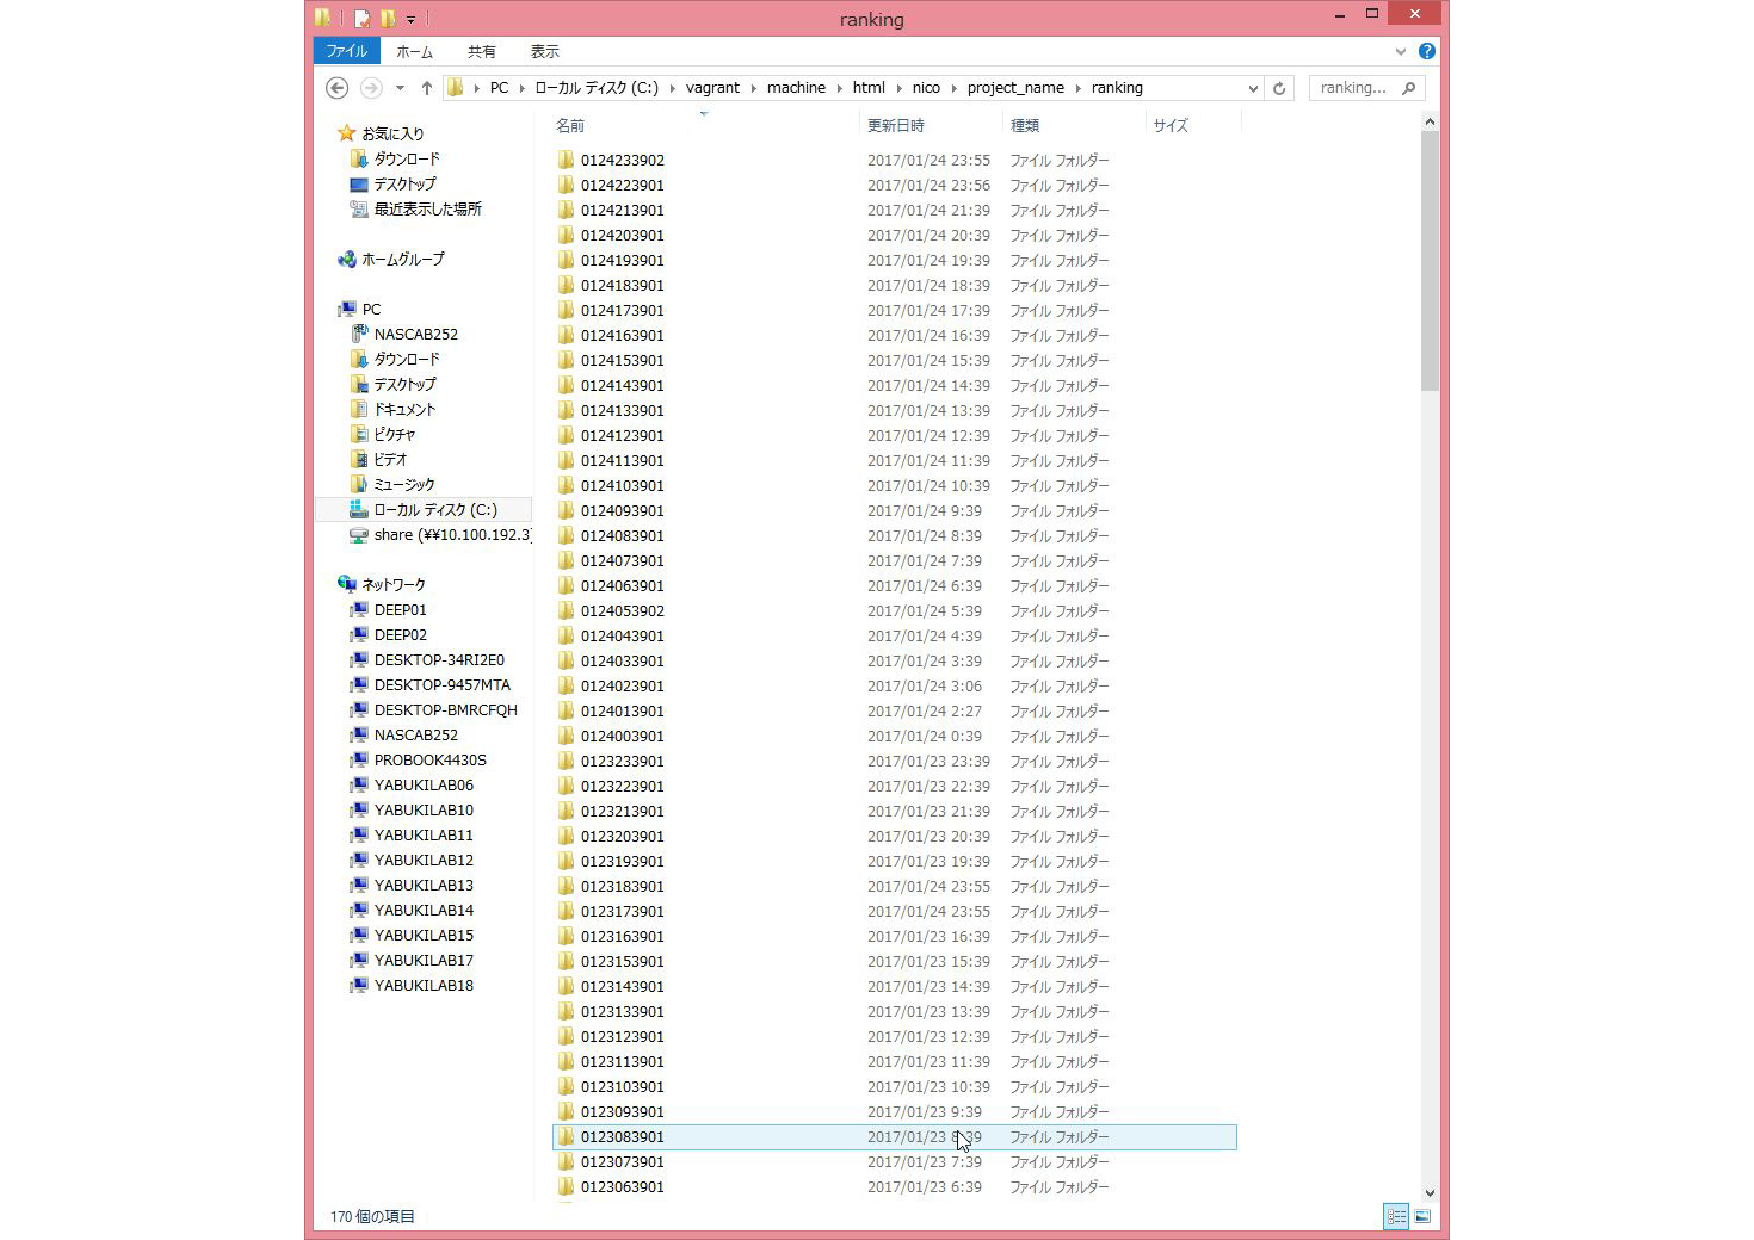
\includegraphics[width=14cm]{kurora01.pdf}
\caption{ranking}\label{ace}
\end{figure}

フォルダ名は実行した月日時分秒となっており,0124043901であれば01月24日04時39分01秒に実行した分のデータとなる.

ニコニコ動画ランキングAPIで収集したデータのディレクトリファイル名はranking

\newpage

\begin{figure}[htb]
\centering
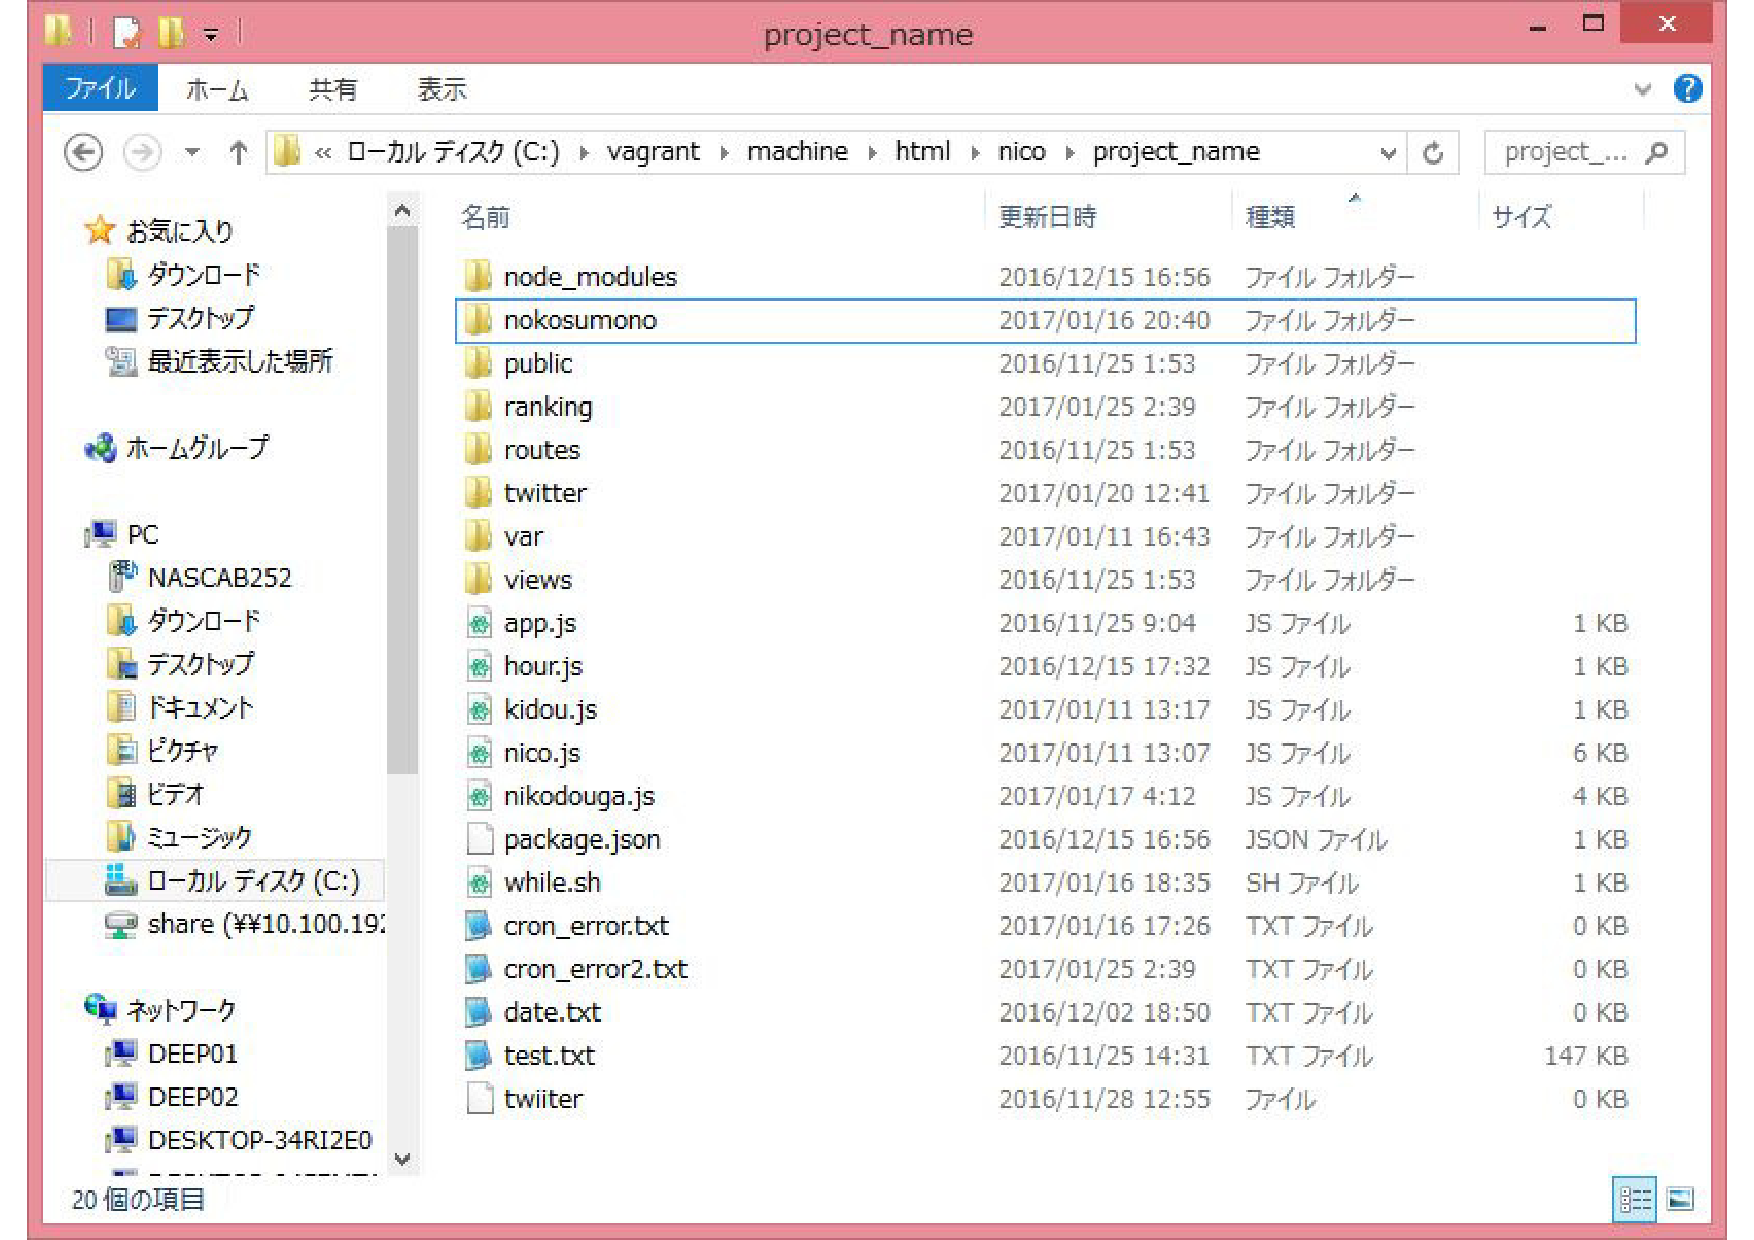
\includegraphics[width=14cm]{fairu01.pdf}
\caption{project name}\label{ace}
\end{figure}


次のディレクトリファイルはproject name.このファイルの中にニコニコ動画ランキングAPIのkidou.jsやモジュールのnico.js,クローラーで動かすwhile.shなどのものがある.
\clearpage

\begin{figure}[htb]
\centering
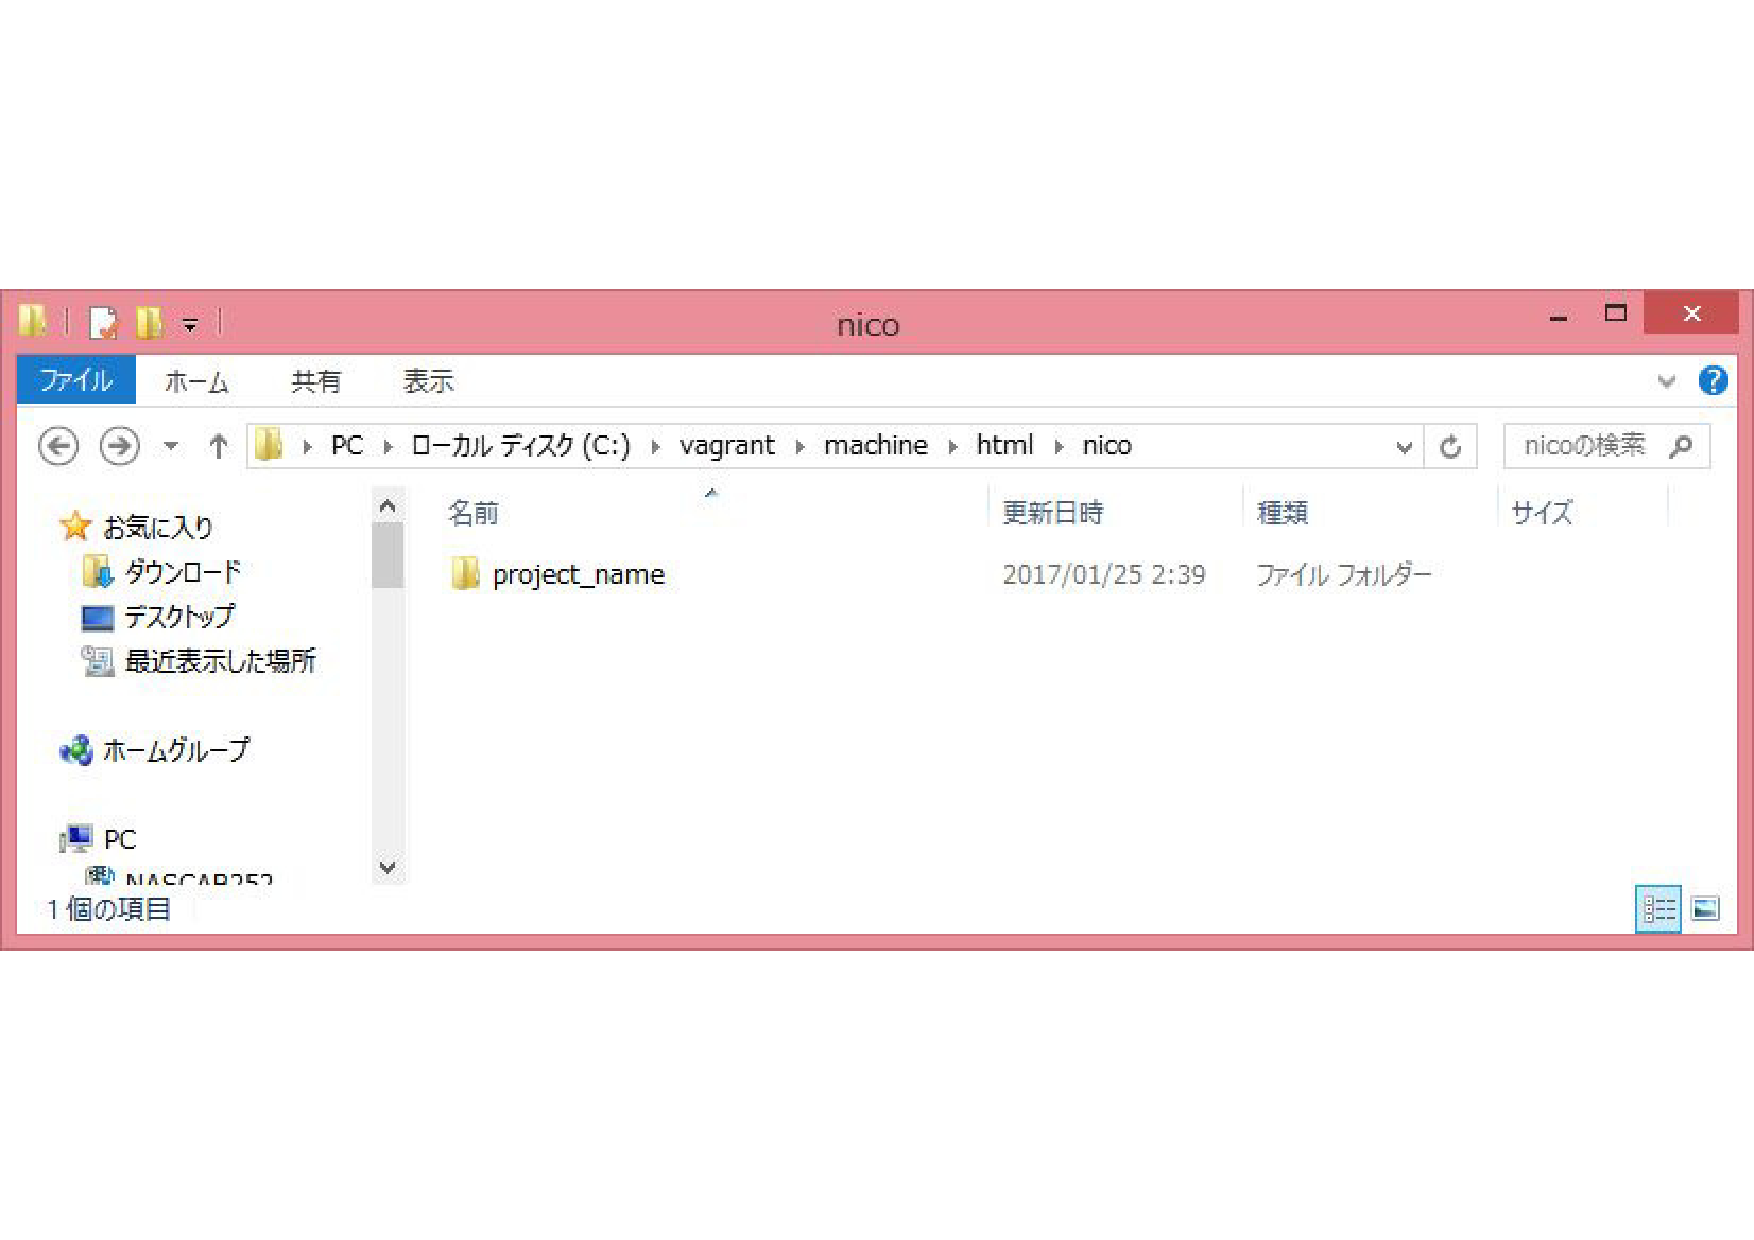
\includegraphics[width=14cm]{fairu02.pdf}
\caption{nico}\label{ace}
\end{figure}


次のディレクトリファイルはnico. このファイルはニコニコ動画ランキングAPIで作られるファイルである.

\clearpage


\begin{figure}[htb]
\centering
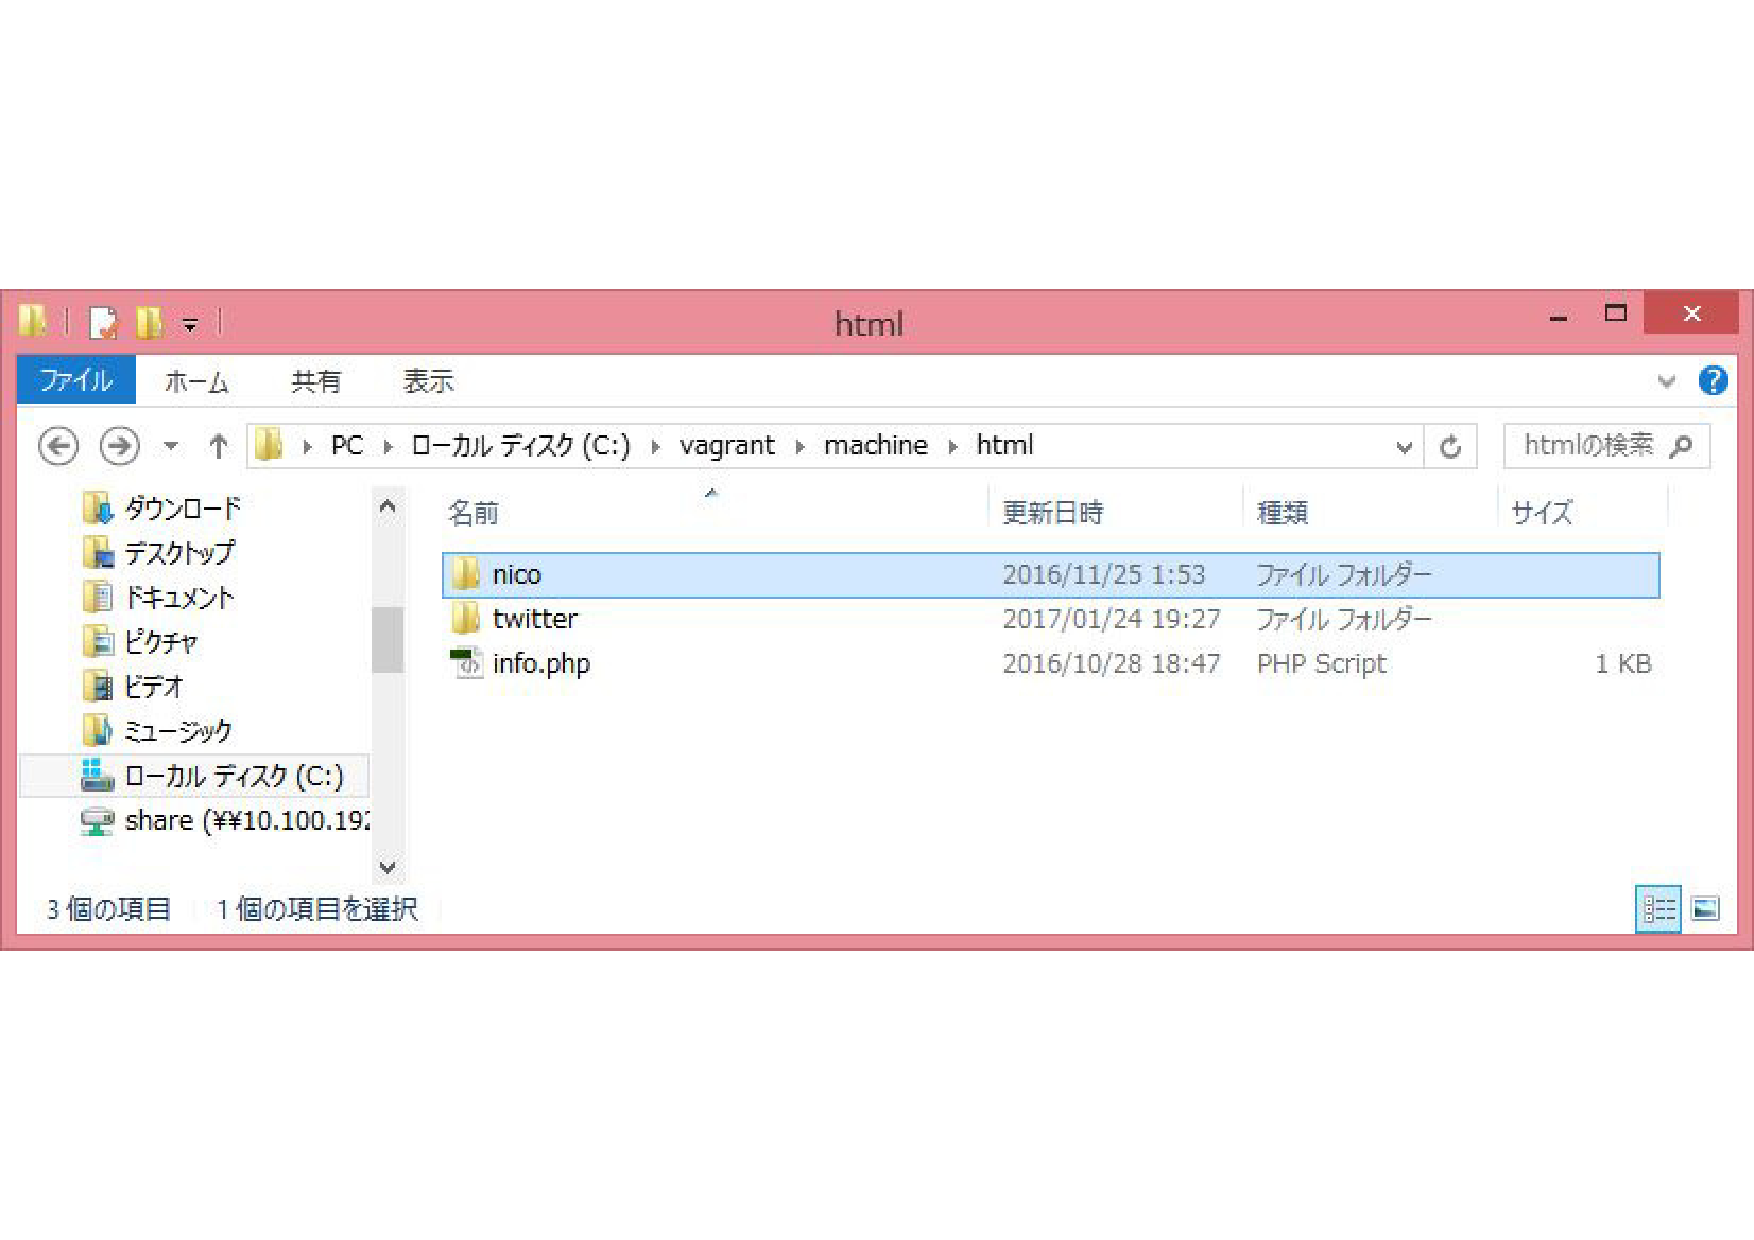
\includegraphics[width=14cm]{fairu03.pdf}
\caption{html}\label{ace}
\end{figure}



次のディレクトリファイルはhtml.ここにはニコニコ動画ランキングのデータ収集用ファイルとTwitterのツイート情報取集用ファイルがある.



\begin{figure}[htb]
\centering
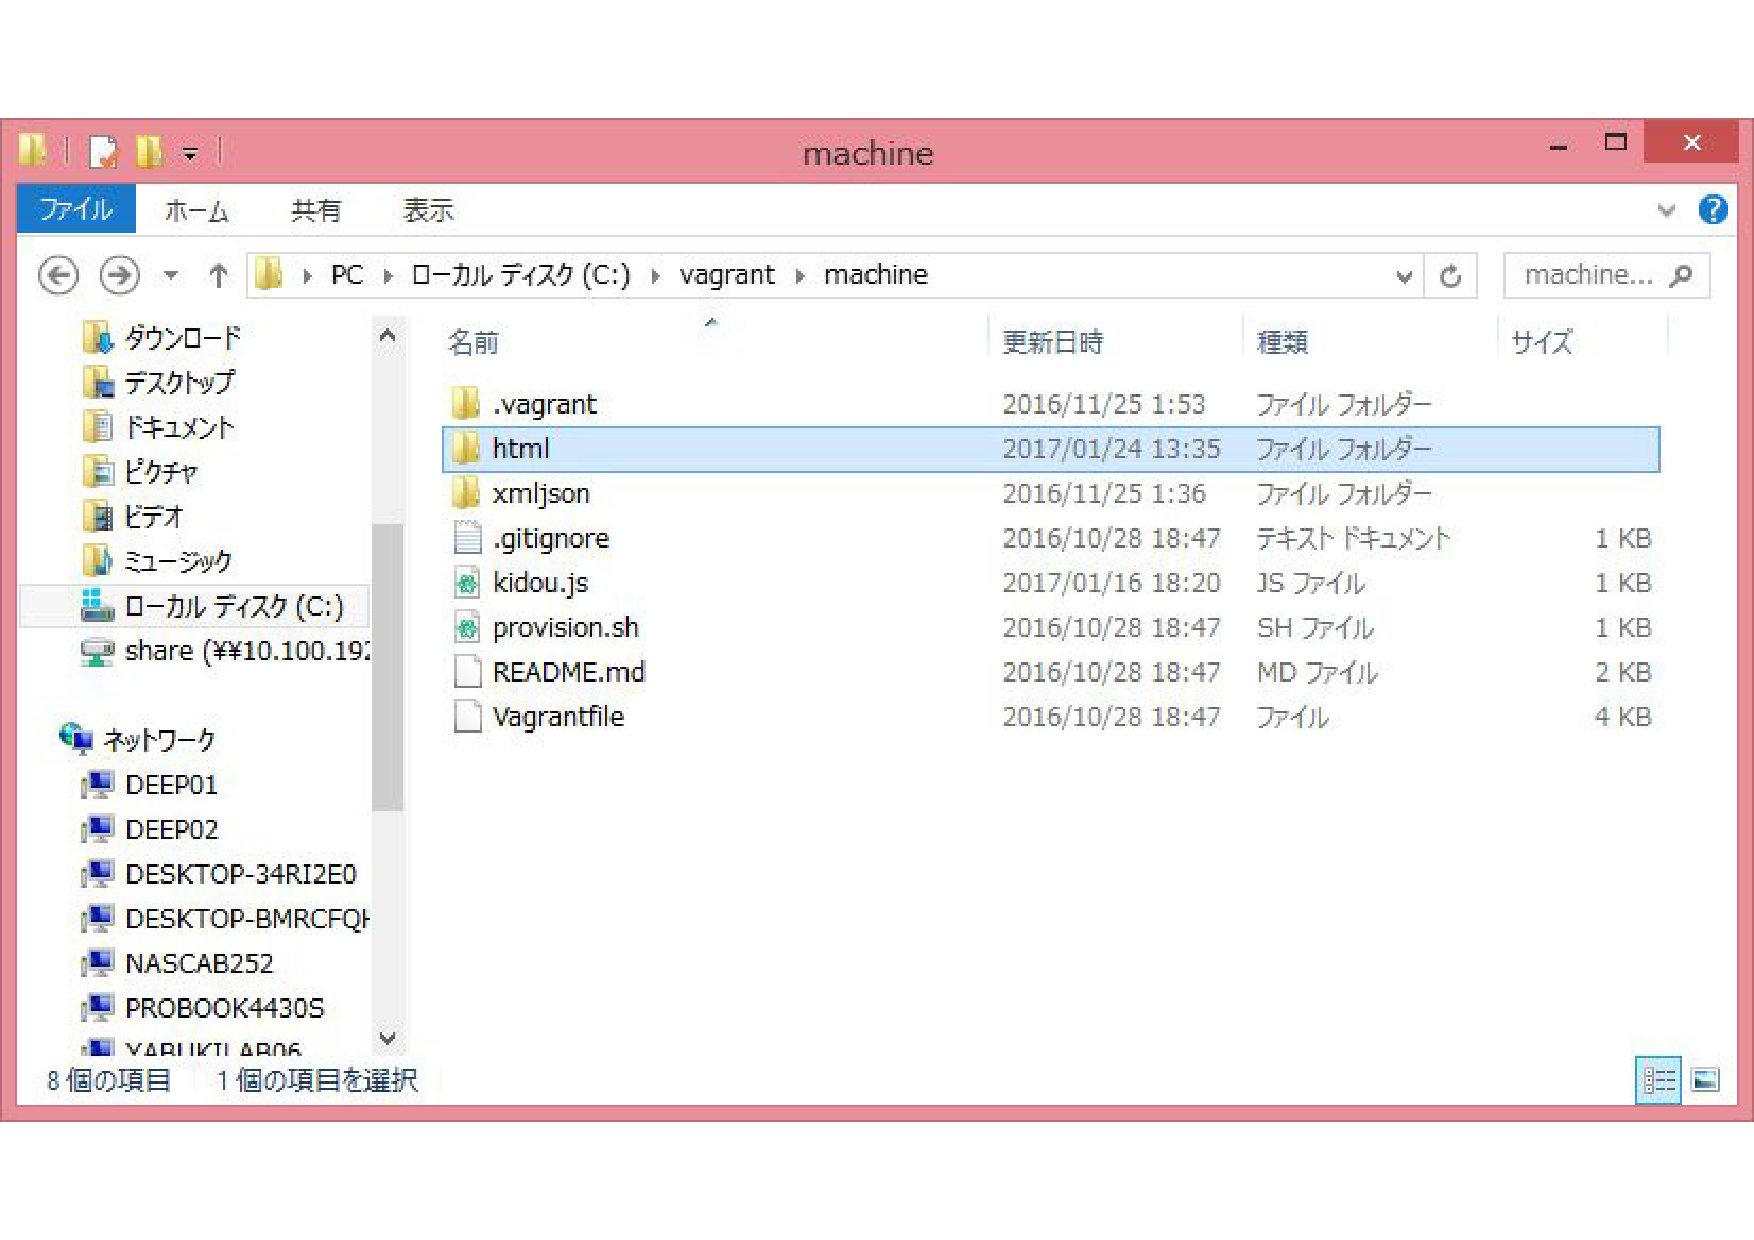
\includegraphics[width=12cm]{fairu04.pdf}
\caption{machine}\label{ace}
\end{figure}

\clearpage

次のディレクトリファイルはmachine.ここにはvagrantの仮想マシンと研究に使う情報を保存しているhtmlがある.

\clearpage

\begin{figure}[htb]
\centering
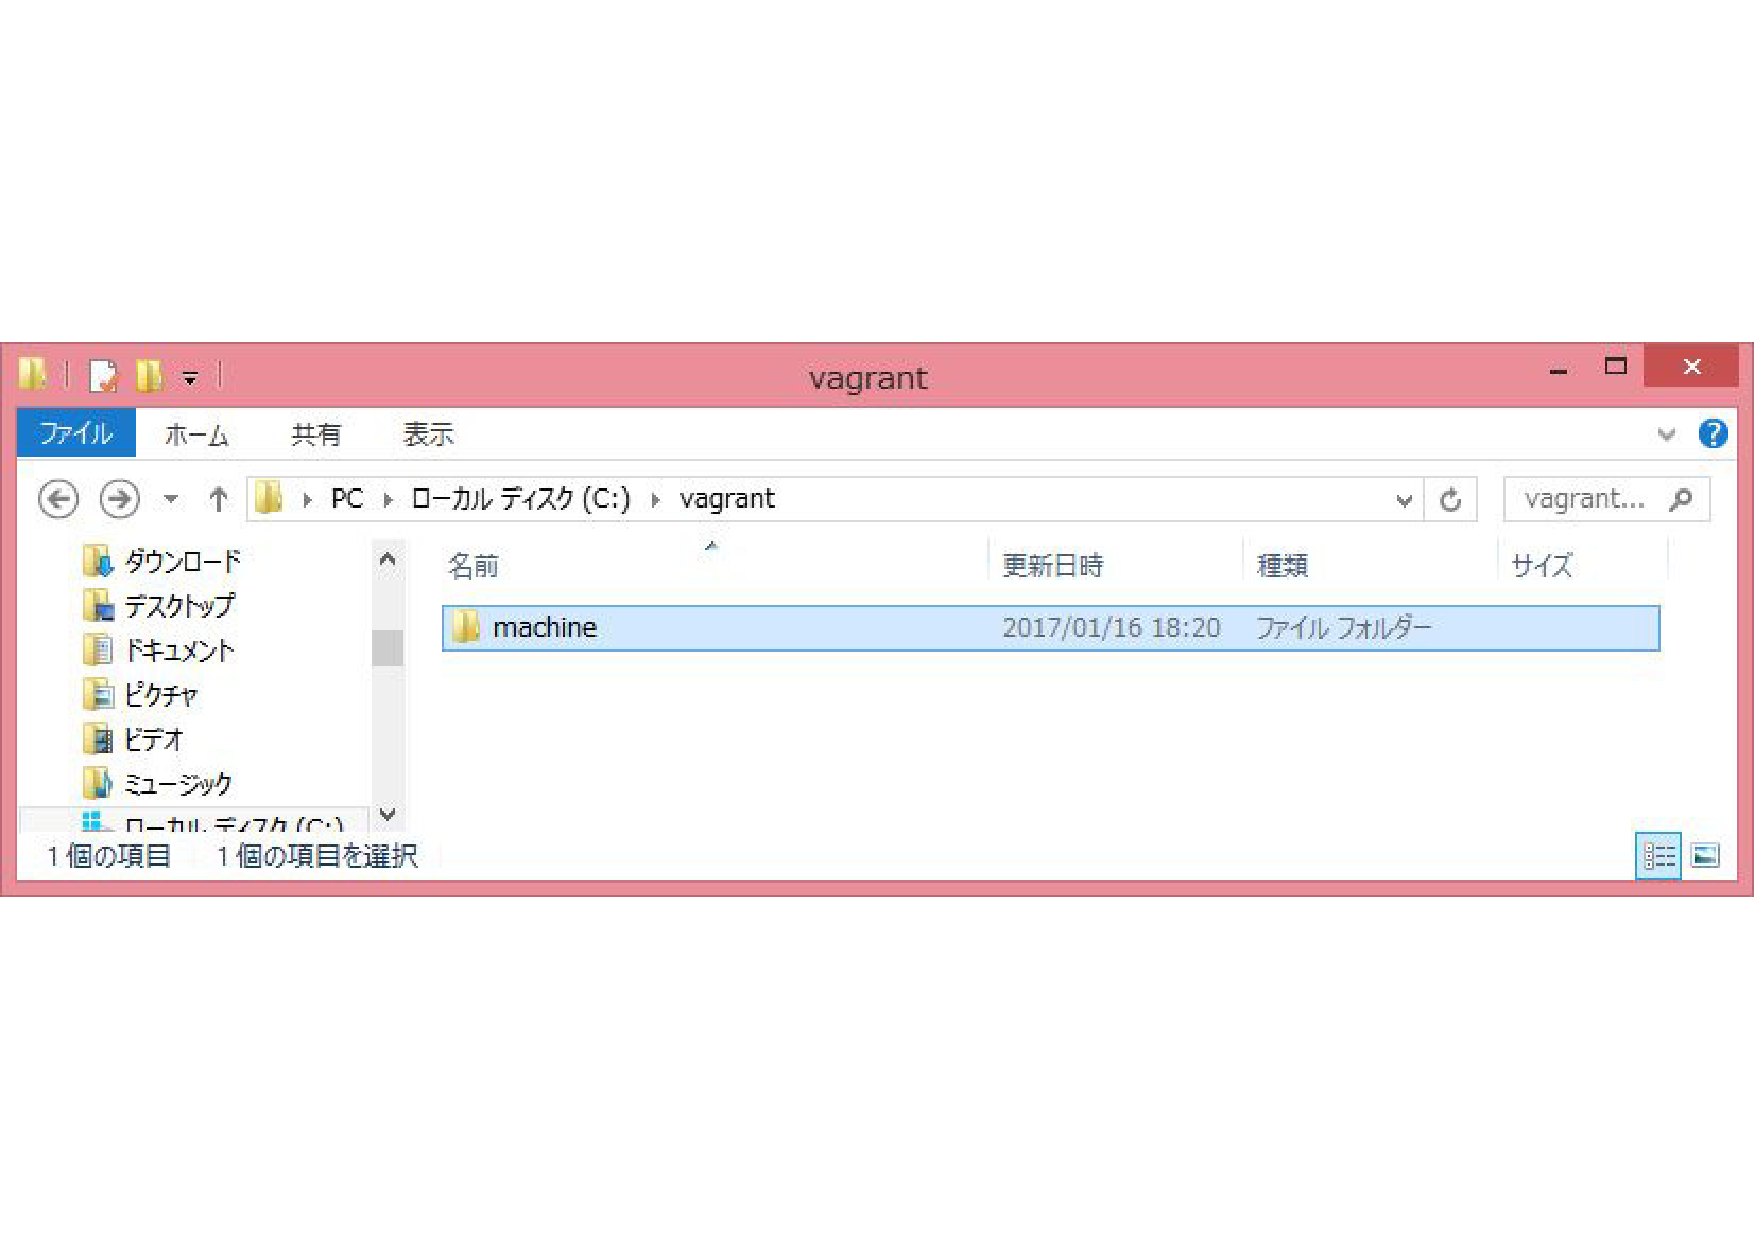
\includegraphics[width=14cm]{fairu05.pdf}
\caption{vagrant}\label{ace}
\end{figure}


次のディレクトリファイルはvgrant.仮想マシンを入れるために作ったmchineがある.

\clearpage

\chapter{回帰分析について}
相関関係や因果関係があると思われる2つの変数のうち、一方の変数から将来的な値を予測するための予測式(回帰直線)を求めるための手法である.2組のデータの傾向を分析するために行われる.
\section{使用したデータについて}

クローラーから得られた情報を元に手作業で日時時間,再生数,再生数の増加,ランキング,ツイート数,ツイート数の増加のデータを打ち込んだ.実際のデータの一部を以下に記載する.

\begin{figure}[htb]
\centering
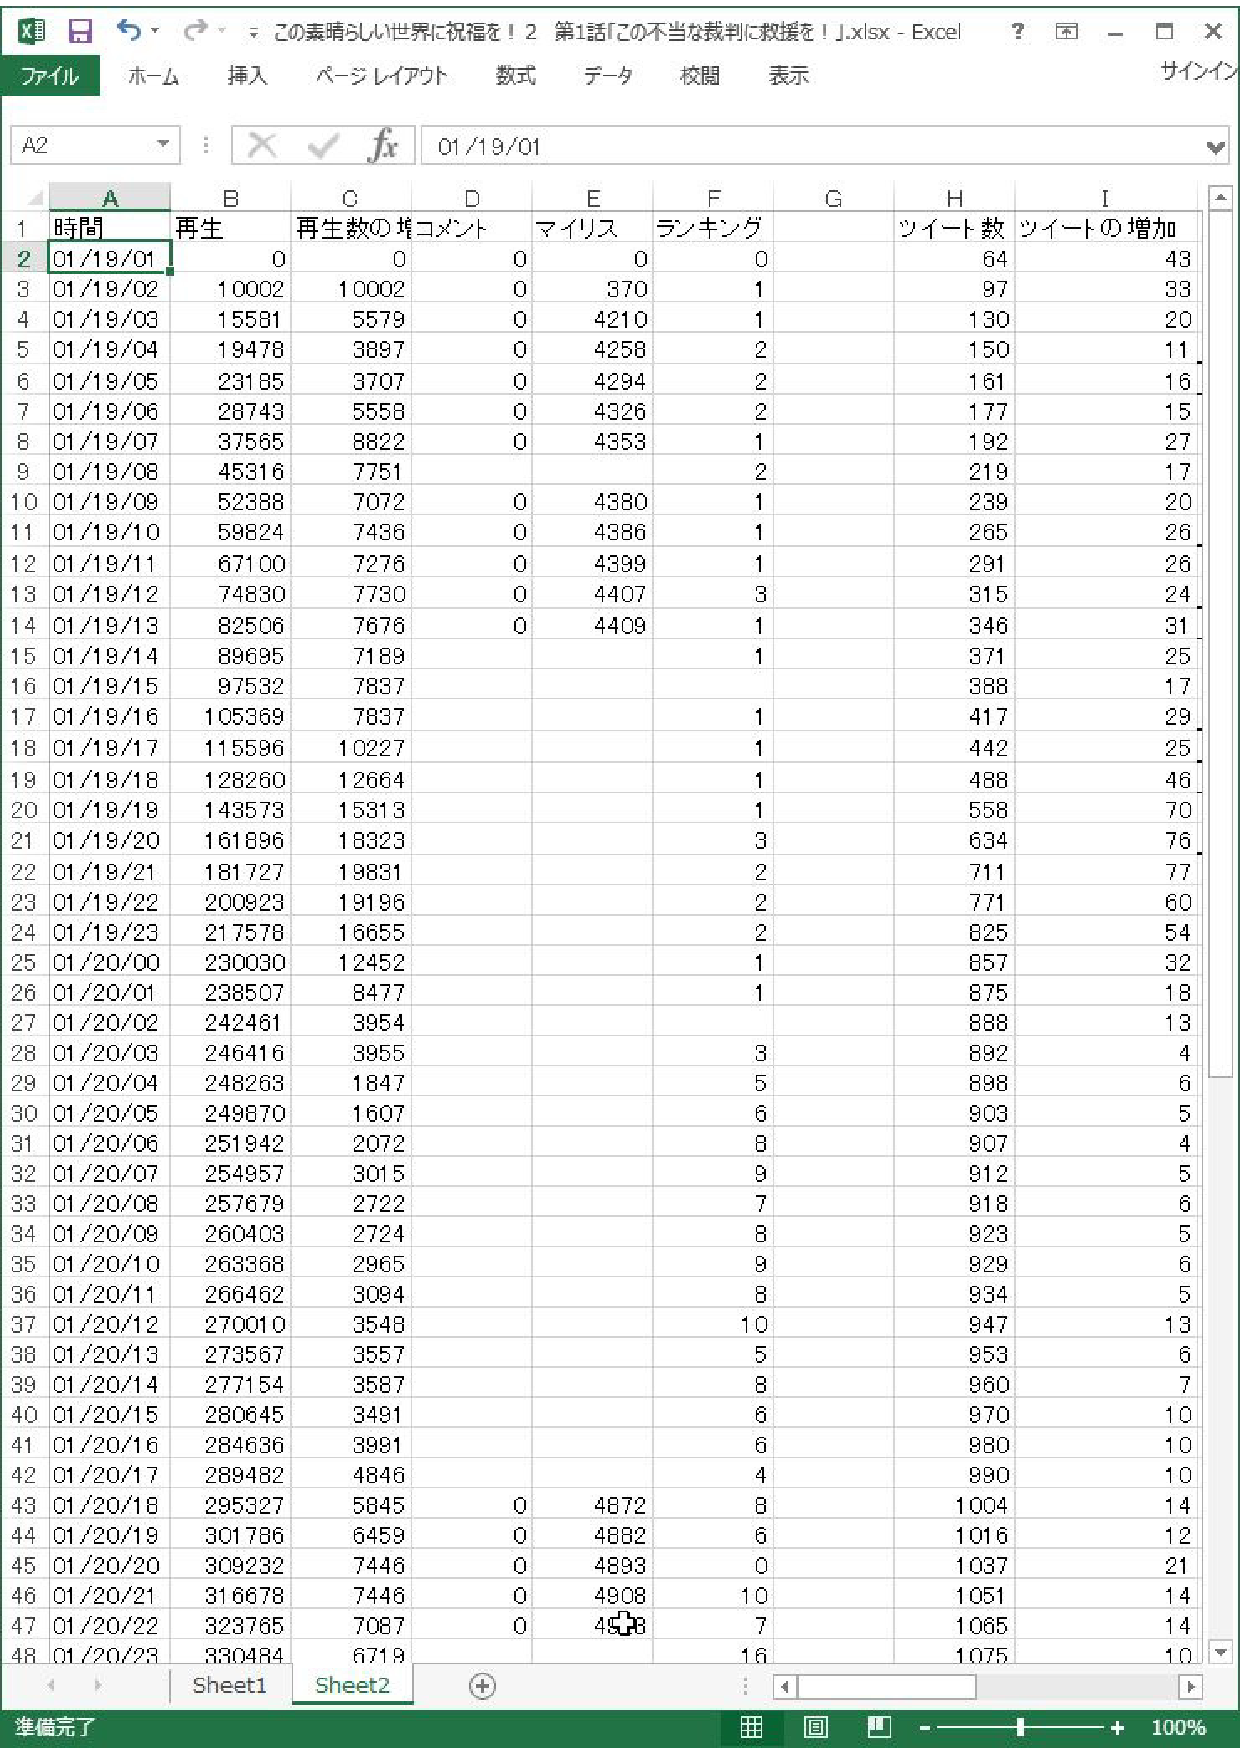
\includegraphics[width=12cm]{de-ta01.pdf}
\caption{エクセルデータ1}\label{ace}
\end{figure}

\clearpage

今回はニコニコ動画のカテゴリ合算毎時総合ランキングに上がっていた動画20件を回帰分析した.回帰分析を行った数値は,動画の再生数とTwitterのツイート数,一時間単位の動画の再生数の増加と一時間ごとのツイート数の増加である.回帰分析の結果の一部を以下に記載する.

\begin{figure}[htb]
\centering
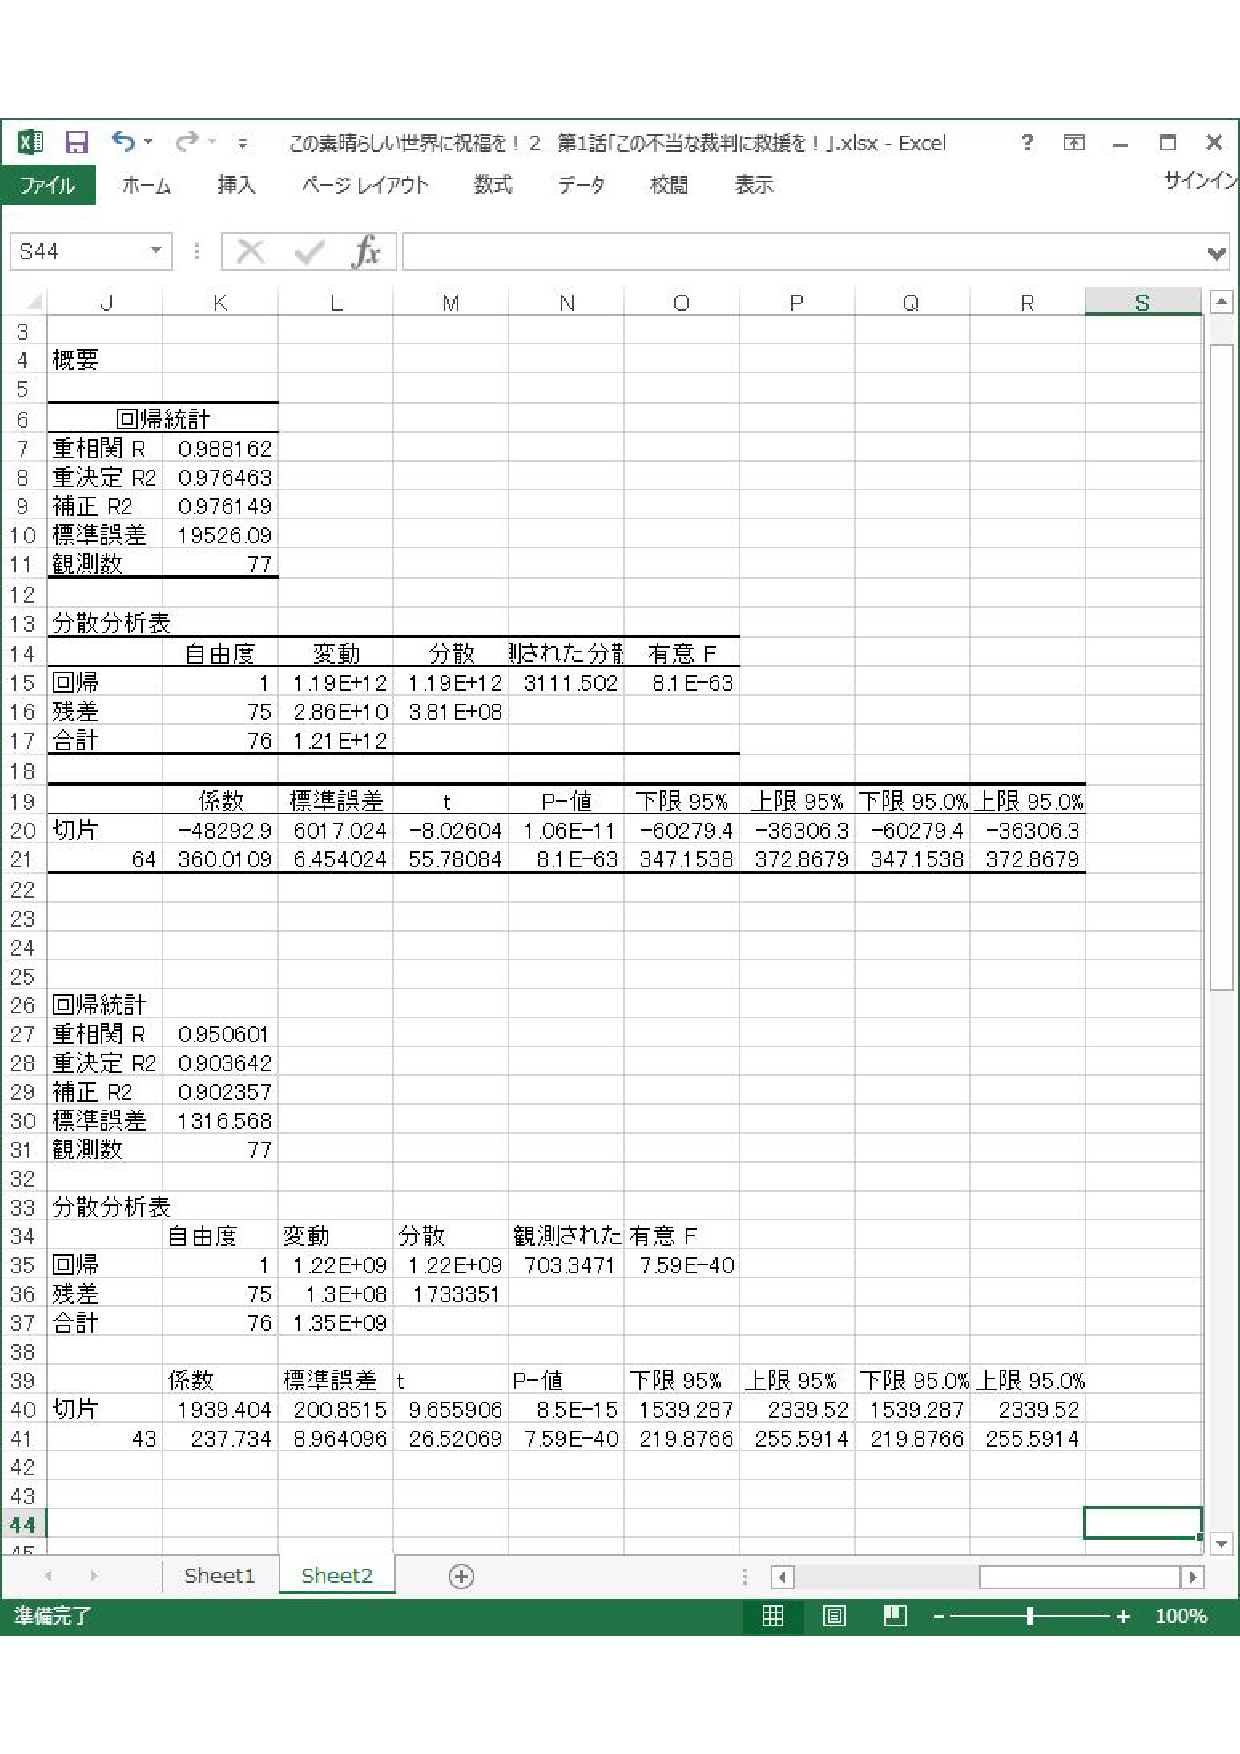
\includegraphics[width=12cm]{de-ta05.pdf}
\caption{エクセルデータ2}\label{ace}
\end{figure}

\clearpage

\section{エクセルでの回帰分析の使い方}
エクセルで回帰分析を行う場合,分析ツールを使用する.まず,エクセルの左上のファイルをクリックする.

\begin{figure}[htb]
\centering
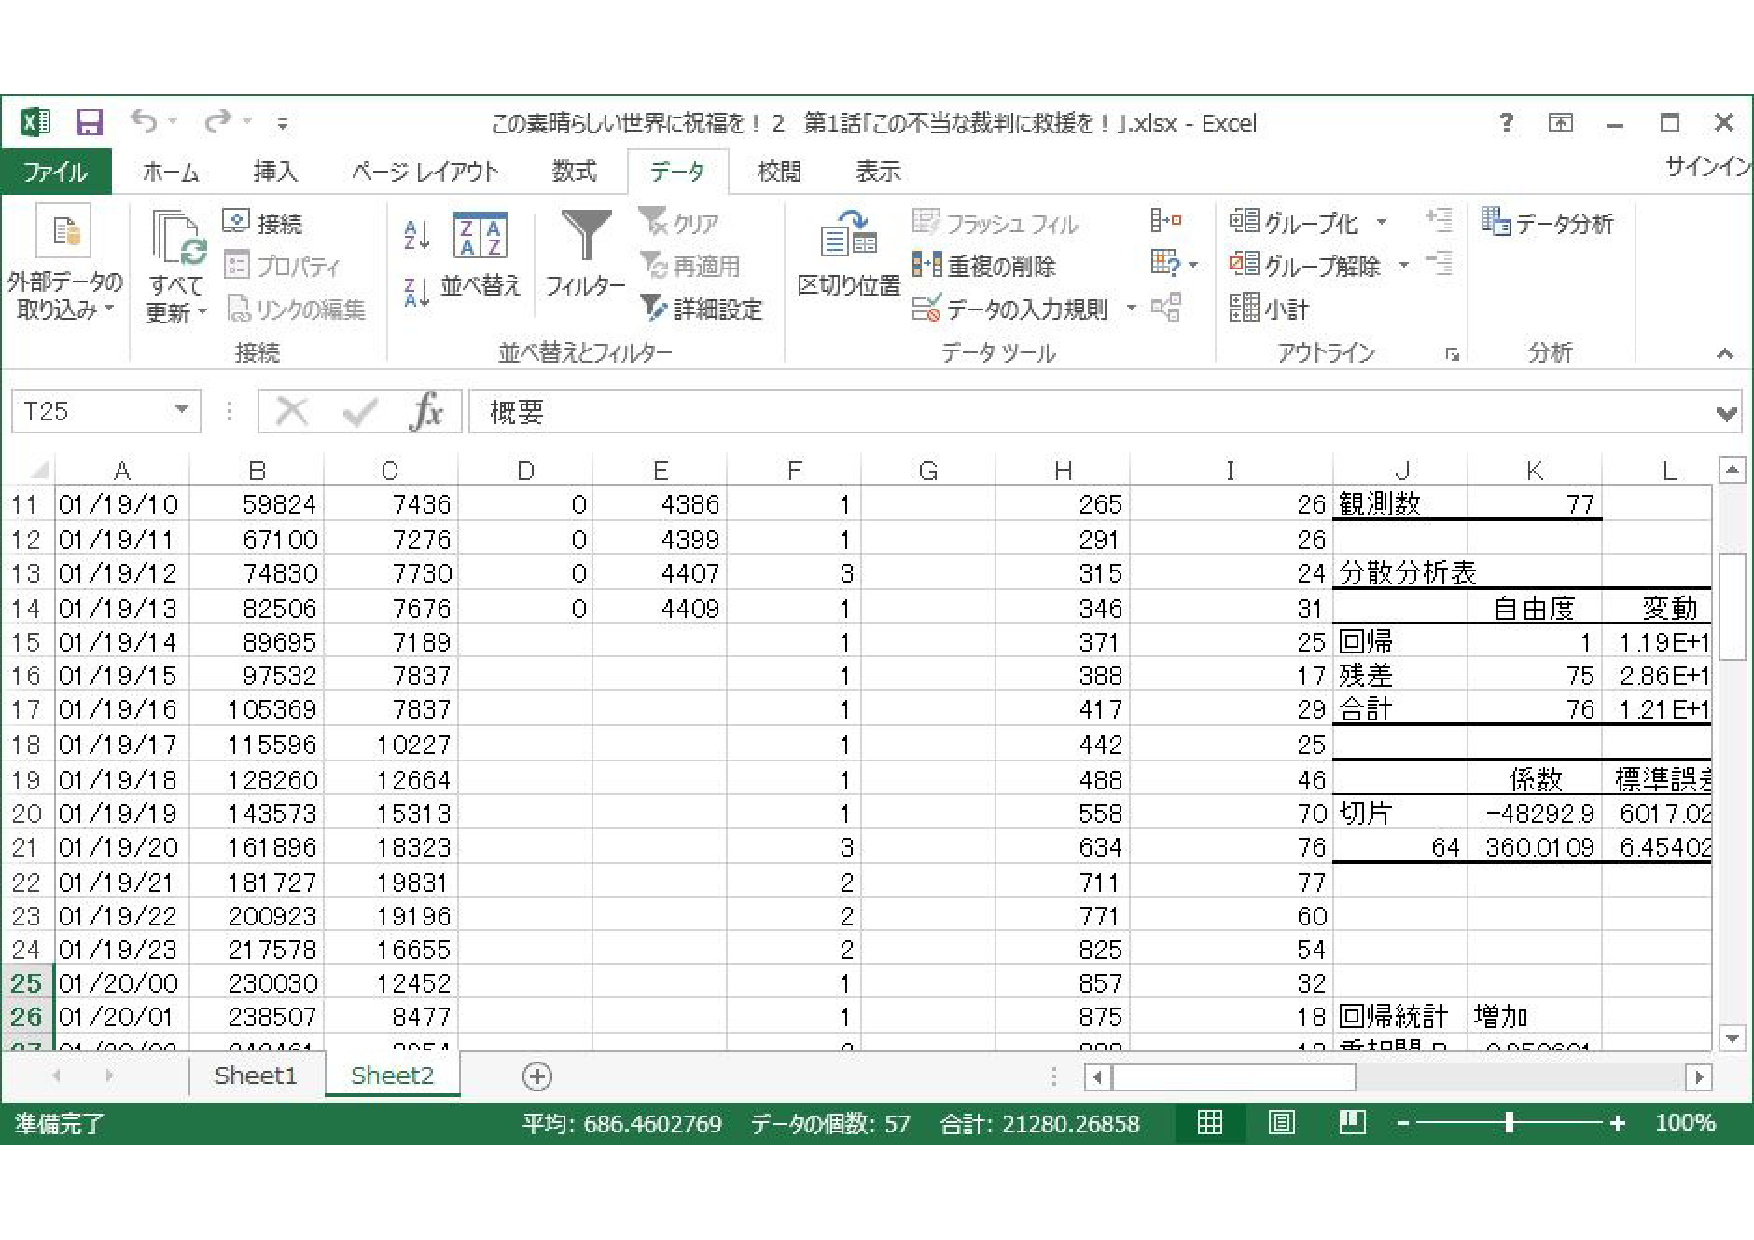
\includegraphics[width=14cm]{ekuseru02.pdf}
\caption{回帰分析1}\label{ace}
\end{figure}

\clearpage

次に,オプションをクリックする.

\begin{figure}[htb]
\centering
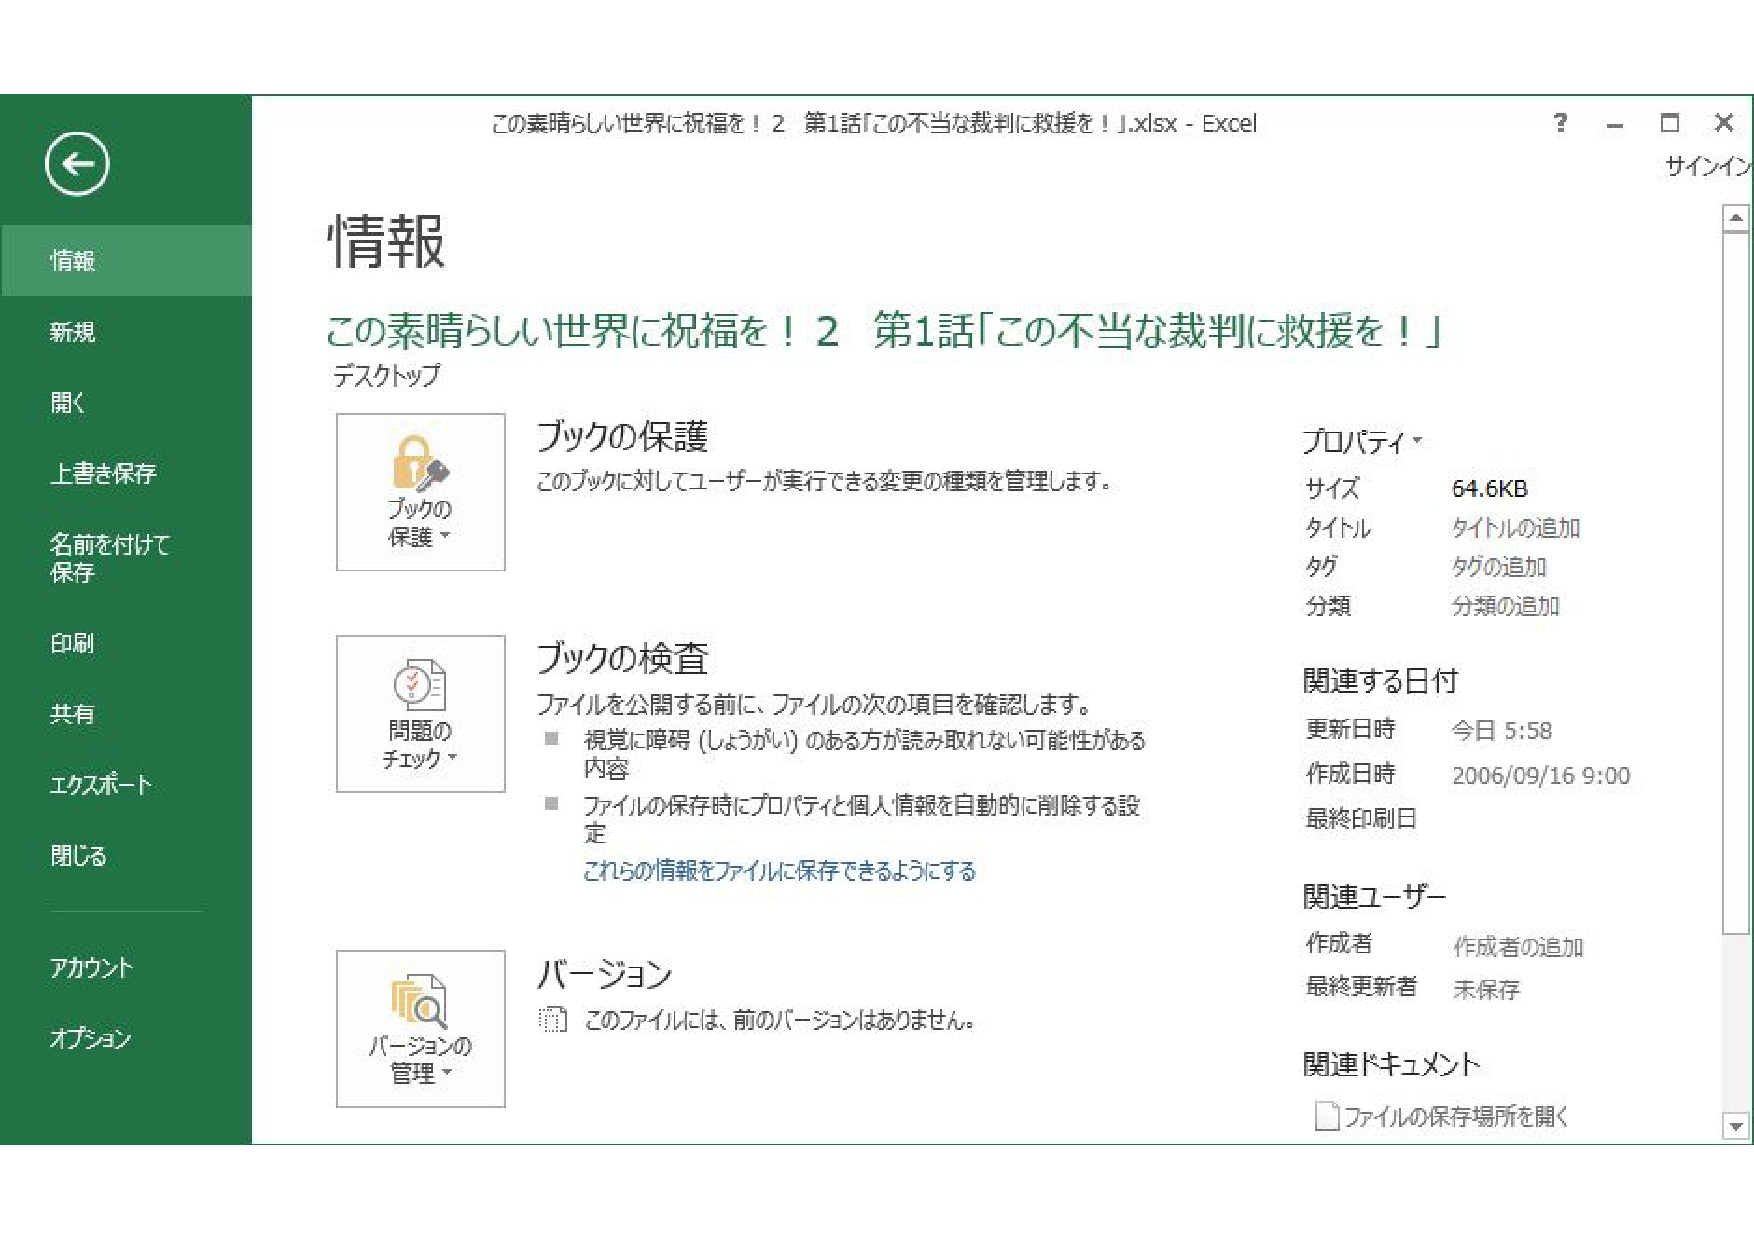
\includegraphics[width=14cm]{ekuseru03.pdf}
\caption{回帰分析2}\label{ace}
\end{figure}

\clearpage

次に,左側のメニューからアドインをクリックし,アドイン表から分析ツールを選択し,OKボタンをクリックする.

\begin{figure}[htb]
\centering
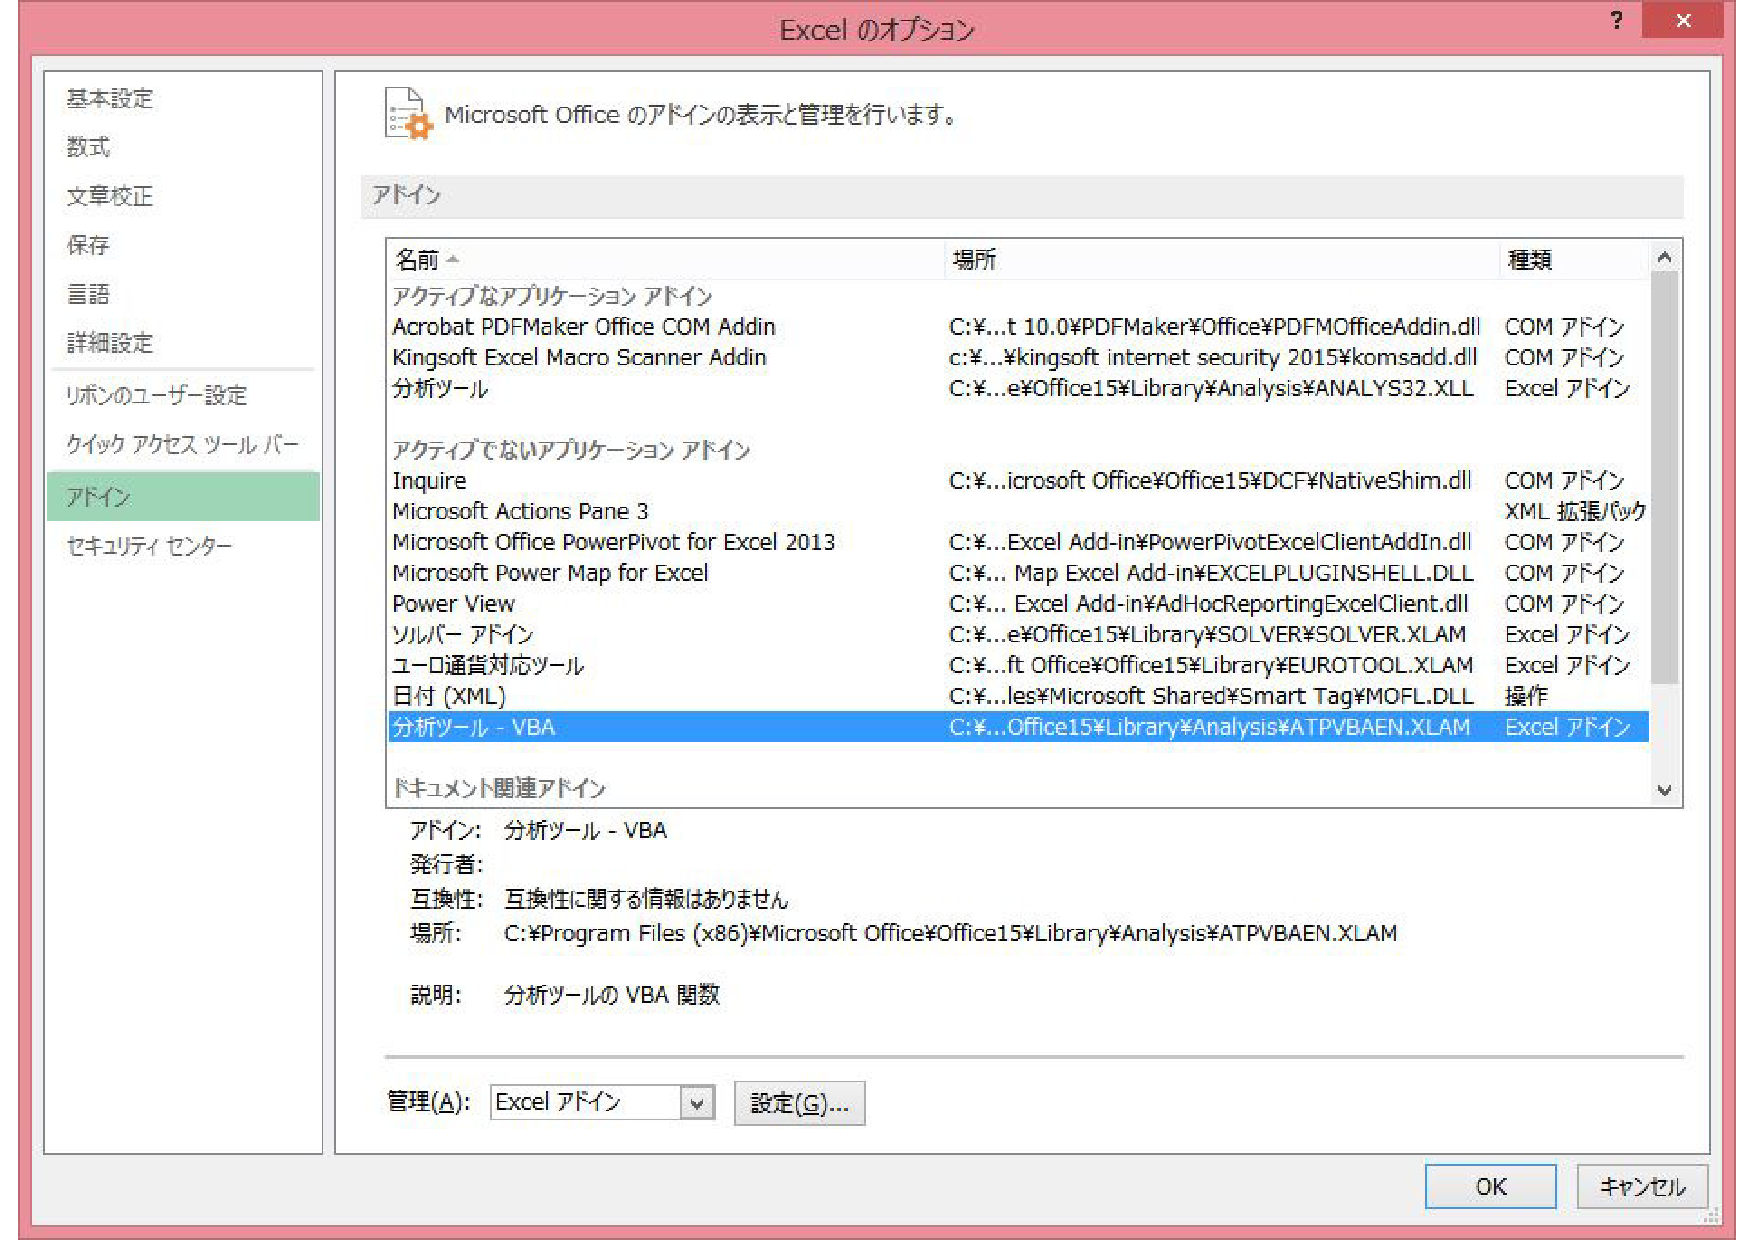
\includegraphics[width=14cm]{ekuseru04.pdf}
\caption{回帰分析3}\label{ace}
\end{figure}

\clearpage

エクセルのタブからデータを選び,右側の分析タブから分析ツールを選択する.

\begin{figure}[htb]
\centering
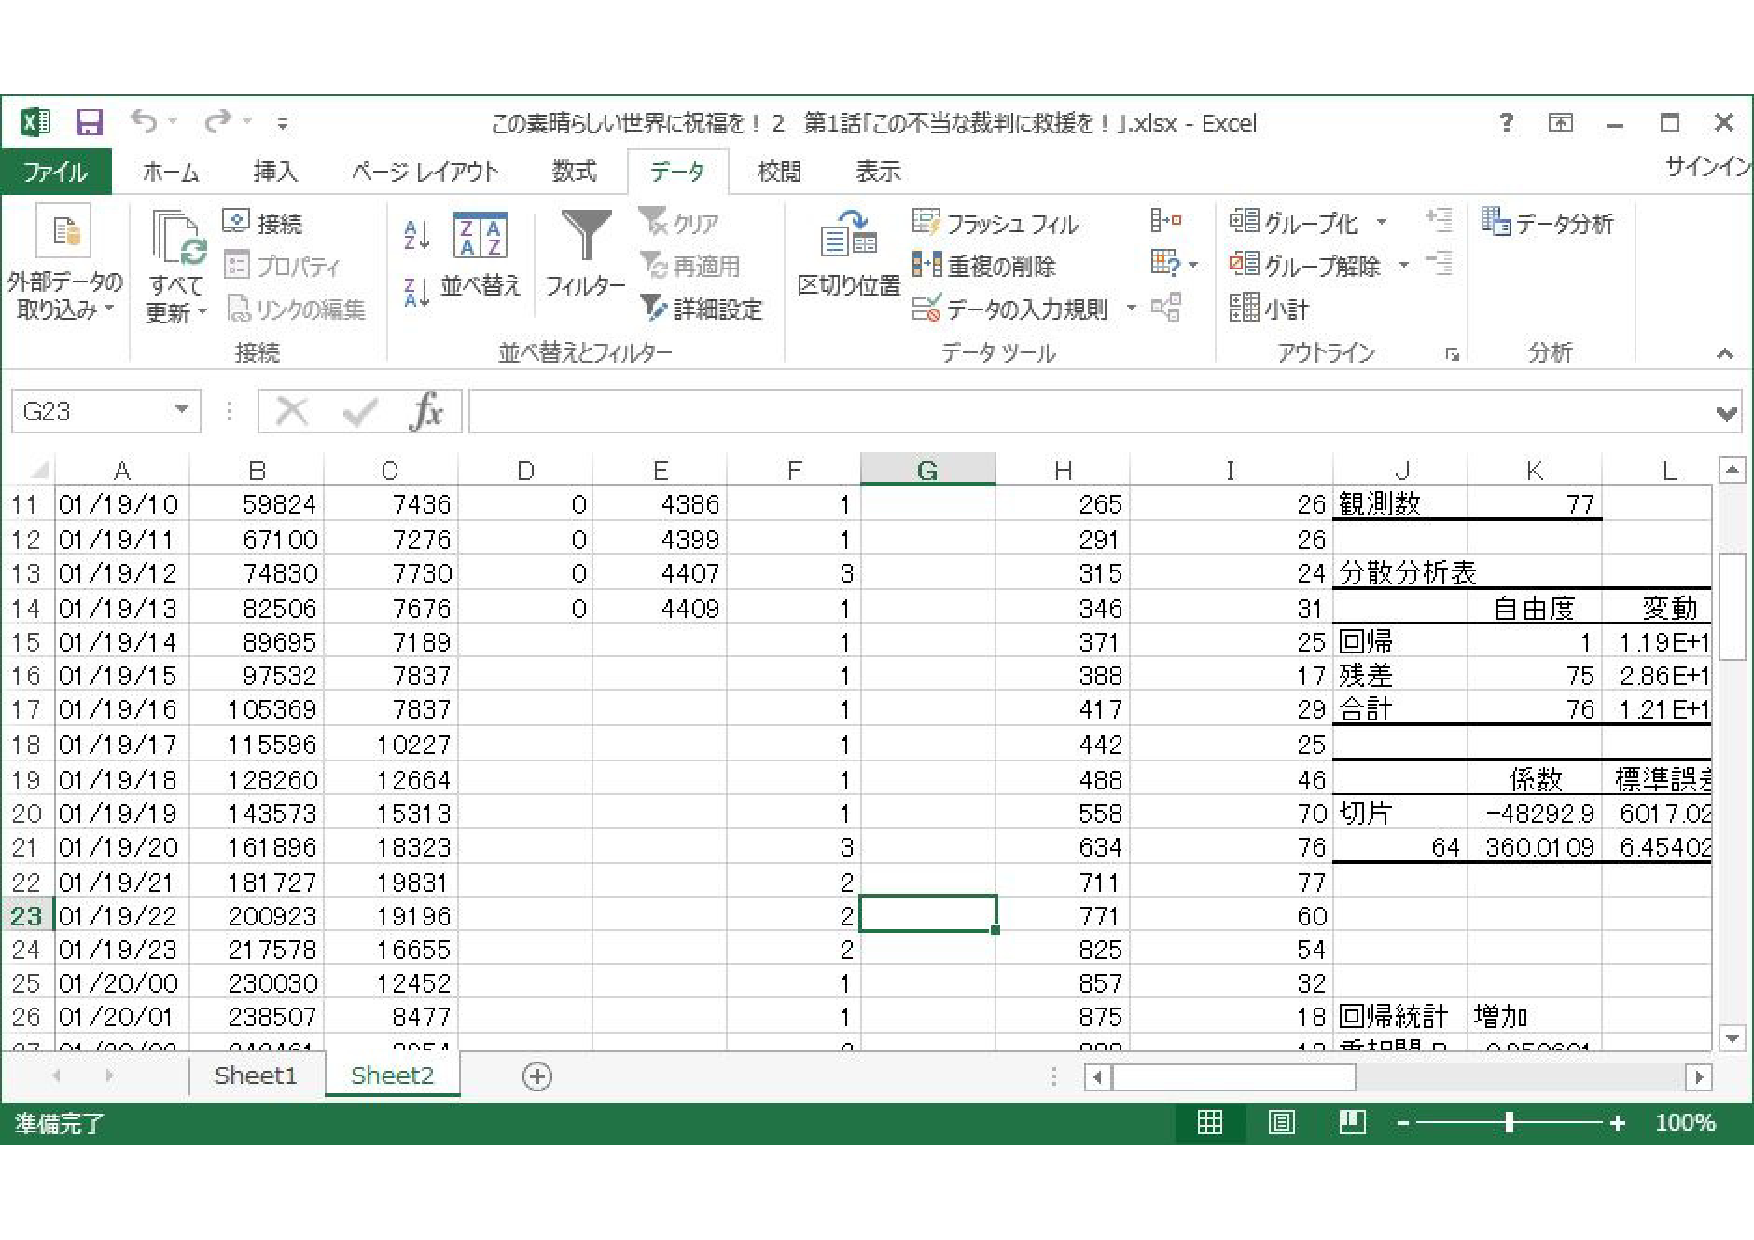
\includegraphics[width=14cm]{ekuseru05.pdf}
\caption{回帰分析4}\label{ace}
\end{figure}

\clearpage

データ分析の表から回帰分析を選択し,Okボタンをクリックする.

\begin{figure}[htb]
\centering
\includegraphics[width=14cm]{ekuseru06.pdf}
\caption{回帰分析5}\label{ace}
\end{figure}

\clearpage

回帰分析を行うため,二つのデータ群を入力Y範囲と入力X範囲に入れ,OKボタンをクリックする..注意として,データは縦書きでないと解析することが出来ない.

\begin{figure}[htb]
\centering
\includegraphics[width=14cm]{ekuseru07.pdf}
\caption{回帰分析6}\label{ace}
\end{figure}

\clearpage

最後にエクセルに回帰分析の結果が書き込まれる.

\begin{figure}[htb]
\centering
\includegraphics[width=14cm]{ekuseru08.pdf}
\caption{回帰分析7}\label{ace}
\end{figure}

\chapter{結果}
結果として,回帰分析を20件行ったところ,動画の再生数とTwitterのツイート数の重相関Rは20件の内20件が0.70以上の数値を出した.一時間単位の動画の再生数の増加と一時間ごとのツイート数の増加の重相関Rは20件の内17件が0,70以上の数値を出した.この結果からニコニコ動画のカテゴリ合算毎時総合ランキングとTwitterのツイートには強い相関関係があることが分かった.
また,動画のカテゴリ合算毎時総合ランキング順位の数値とTwitterのツイート数と一時間ごとのツイート増加数の回帰分析を行った.結果はツイート数の重相関Rは0.2から0.4の数値が20件の内4件,0.4から0.7の数値が20件の内16件,ツイートの増加数の重相関Rは0.2から0.4の数値が20件の内3件,0.4から0.7の数値が20件の内15件,0,7以上が20件の内2件となった.
\chapter{考察}
ニコニコ動画の再生数を上げることにTwitterを使う場合,強い相関関係があり,カテゴリ合算毎時総合ランキングを上げるためにTwitterを使用することにはかなり相関関係があることが分かった.そのためランキングの維持や動画の再生数を上げたい場合にはTwitterを使用すればいいことが考えられる.また,本研究ではTwitterを使用したが,ニコニコ動画の動画画面にはtwitterのアイコンの他にFacebookとLINEのアイコンが存在する.そのためFacebookとLINEでも同様な研究が必要であると考えた.
\chapter{結論}
ニコニコ動画の視聴ランキングと動画関連ツイートの相関性はかなり相関関係がある.また,ニコニコ動画の再生数とTwitterのツイート数には強い相関関係があり,ニコニコ動画の一時間ごとの再生増加数とTwitterの一時間ごとのツイート増加数には強い相関関係がある.そのため,Twitterを使用しニコニコ動画に投稿した動画を知らせることは優良である.しかし,FacebookとLINEのアイコンがニコニコ動画の動画画面で確認できるため,FacebookとLINEでも同様な研究が必要であるという課題が出てきた.


\noindent
□□□□□□□□□■□□□□□□□□□■□□□□□□□□□■□□□□□□□□□■
□□□□□□□□□■□□□□□□□□□■□□□□□□□□□■□□□□□□□□□■
□□□□□□□□□■□□□□□□□□□■□□□□□□□□□■□□□□□□□□□■
□□□□□□□□□■□□□□□□□□□■□□□□□□□□□■□□□□□□□□□■
□□□□□□□□□■□□□□□□□□□■□□□□□□□□□■□□□□□□□□□■
□□□□□□□□□■□□□□□□□□□■□□□□□□□□□■□□□□□□□□□■
□□□□□□□□□■□□□□□□□□□■□□□□□□□□□■□□□□□□□□□■
□□□□□□□□□■□□□□□□□□□■□□□□□□□□□■□□□□□□□□□■
□□□□□□□□□■□□□□□□□□□■□□□□□□□□□■□□□□□□□□□■
□□□□□□□□□■□□□□□□□□□■□□□□□□□□□■□□□□□□□□□■
□□□□□□□□□■□□□□□□□□□■□□□□□□□□□■□□□□□□□□□■
□□□□□□□□□■□□□□□□□□□■□□□□□□□□□■□□□□□□□□□■
□□□□□□□□□■□□□□□□□□□■□□□□□□□□□■□□□□□□□□□■
□□□□□□□□□■□□□□□□□□□■□□□□□□□□□■□□□□□□□□□■
□□□□□□□□□■□□□□□□□□□■□□□□□□□□□■□□□□□□□□□■
□□□□□□□□□■□□□□□□□□□■□□□□□□□□□■□□□□□□□□□■
□□□□□□□□□■□□□□□□□□□■□□□□□□□□□■□□□□□□□□□■
□□□□□□□□□■□□□□□□□□□■□□□□□□□□□■□□□□□□□□□■
□□□□□□□□□■□□□□□□□□□■□□□□□□□□□■□□□□□□□□□■
□□□□□□□□□■□□□□□□□□□■□□□□□□□□□■□□□□□□□□□■
□□□□□□□□□■□□□□□□□□□■□□□□□□□□□■□□□□□□□□□■
□□□□□□□□□■□□□□□□□□□■□□□□□□□□□■□□□□□□□□□■
□□□□□□□□□■□□□□□□□□□■□□□□□□□□□■□□□□□□□□□■
□□□□□□□□□■□□□□□□□□□■□□□□□□□□□■□□□□□□□□□■
□□□□□□□□□■□□□□□□□□□■□□□□□□□□□■□□□□□□□□□■
□□□□□□□□□■□□□□□□□□□■□□□□□□□□□■□□□□□□□□□■
□□□□□□□□□■□□□□□□□□□■□□□□□□□□□■□□□□□□□□□■
□□□□□□□□□■□□□□□□□□□■□□□□□□□□□■□□□□□□□□□■
□□□□□□□□□■□□□□□□□□□■□□□□□□□□□■□□□□□□□□□■
□□□□□□□□□■□□□□□□□□□■□□□□□□□□□■□□□□□□□□□■
□□□□□□□□□■□□□□□□□□□■□□□□□□□□□■□□□□□□□□□■
□□□□□□□□□■□□□□□□□□□■□□□□□□□□□■□□□□□□□□□■
□□□□□□□□□■□□□□□□□□□■□□□□□□□□□■□□□□□□□□□■
□□□□□□□□□■□□□□□□□□□■□□□□□□□□□■□□□□□□□□□■
□□□□□□□□□■□□□□□□□□□■□□□□□□□□□■□□□□□□□□□■
□□□□□□□□□■□□□□□□□□□■□□□□□□□□□■□□□□□□□□□■
□□□□□□□□□■□□□□□□□□□■□□□□□□□□□■□□□□□□□□□■
□□□□□□□□□■□□□□□□□□□■□□□□□□□□□■□□□□□□□□□■
□□□□□□□□□■□□□□□□□□□■□□□□□□□□□■□□□□□□□□□■
■■■■■■■■■■■■■■■■■■■■■■■■■■■■■■■■■■■■■■■■
□□□□□□□□□■□□□□□□□□□■□□□□□□□□□■□□□□□□□□□■

\bibliographystyle{junsrt}
\bibliography{biblio}%「biblio.bib」というファイルが必要.

\chapter*{謝辞}\addcontentsline{toc}{chapter}{謝辞}

本研究を進めるにあたり,矢吹研究室矢吹太朗准教授には,多くの時間をご指導にさいて頂きました.
また矢吹研究室の皆様には,多くの知識や示唆を頂きました.協力していただい皆様に感謝の気持ちと御礼を申し上げます.

\end{document}
